\documentclass[aspectratio=169,xcolor=table]{beamer}
\usetheme{Madrid}
\usecolortheme{default}
\setbeamertemplate{navigation symbols}{}

% Essential Packages
\usepackage{graphicx}
\usepackage{amsmath}
\usepackage{amssymb}
\usepackage{siunitx}
\usepackage{hyperref}
\usepackage{appendixnumberbeamer}
\usepackage{booktabs}
\usepackage{tabularx}
\usepackage{array}
\setbeamercovered{transparent=15}
% ------------------------------------------------------------
% Equal box macro (\qbox) for Dynamic & Mode ID slides
% ------------------------------------------------------------
\newlength{\qboxwidth}
\setlength{\qboxwidth}{0.485\textwidth}
\newlength{\qboxbodyH}
\newlength{\tmpH}
\newsavebox{\qboxA}
\newsavebox{\qboxB}
\newsavebox{\qboxC}
\newsavebox{\qboxD}

\newcommand{\qboxmeasure}[2]{%
  \begin{minipage}{\dimexpr\qboxwidth-1.5ex\relax}%
    \footnotesize
    \begin{itemize}#2\end{itemize}%
  \end{minipage}%
}

\newcommand{\qbox}[3][\qboxbodyH]{%
  \begin{block}{#2}%
    \begin{minipage}[t][#1][t]{\linewidth}%
      \footnotesize
      \begin{itemize}#3\end{itemize}%
    \end{minipage}%
  \end{block}%
}

% ------------------------------------------------------------
% Helpers for the NBI+ECH (left) | NBI-only (right) layouts
% ------------------------------------------------------------
\newcolumntype{C}[1]{>{\centering\arraybackslash}m{#1}}
\newcommand{\winA}{\textbf{NBI + ECH} {\scriptsize(\SIrange{259.1}{291.3}{ms})}}
\newcommand{\winB}{\textbf{NBI only} {\scriptsize(\SIrange{291.3}{300.0}{ms})}}
\newcommand{\colhead}[1]{%
    \begin{beamercolorbox}[wd=\linewidth,sep=0.6ex,center]{block title}#1\end{beamercolorbox}}
\newcommand{\incl}{{\scriptsize\textcolor{red!70!black}{(inconclusive)}}}
\definecolor{primcol}{RGB}{214,39,40}
\definecolor{seccol}{RGB}{230,120,0}
\newcommand{\Prim}{\textcolor{primcol}{\textbf{Primary}}}
\newcommand{\Sec}{\textcolor{seccol}{\textbf{Secondary}}}

% Title and Author Information
\title[MHD Oscillations at Heliotron J]{Analysis of magnetohydrodynamics oscillations \\ at Heliotron J with Python}
\author[K. Rishor Villalobos]{Kevin Enrique Rishor Villalobos}
\institute[TEC \& IAE Kyoto]{
    Physics School, Tecnológico de Costa Rica (TEC) \\
    \vspace{0.2cm}
    Institute of Advanced Energy, Kyoto University
}
\date{September, 2026}

% Logos on Title Page
\titlegraphic{
    
\includegraphics[height=1.5cm]{Images/Tec.png} \hspace{2cm}
    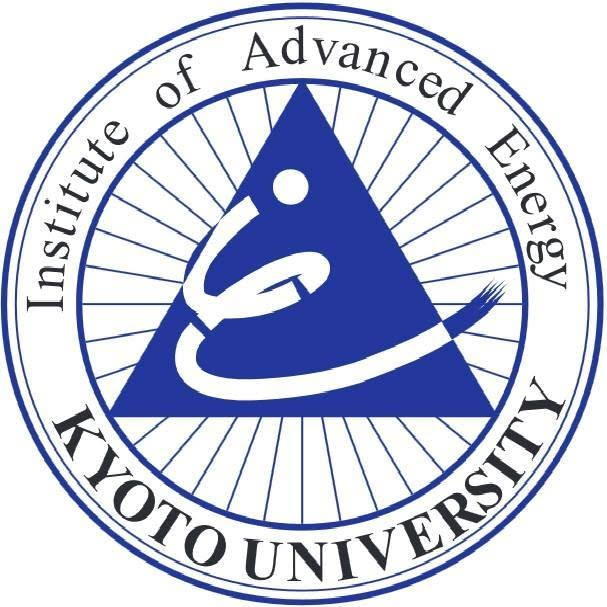
\includegraphics[height=1.5cm]{Images/IAE.jpg}
}

\begin{document}

% ============================================================
% 1 -- Title
% ============================================================
\begin{frame}
    \titlepage
\end{frame}

% ============================================================
\section{Motivation \& Objectives}
% ============================================================

% Motivation + objectives, five items revealed one at a time
\begin{frame}{Motivation \& Objectives}
    \footnotesize
    \onslide<1->{%
    \textbf{General objective:} characterize MHD oscillations in Heliotron J through
    Python-based analysis, to determine their excitation mechanisms and assess their
    impact on plasma confinement.}

    \vspace{0.15cm}
    \onslide<2->{\textbf{Specific objectives, one shot (\#88653):}}
    \begin{enumerate}
        \item<2-> \textbf{Spectral properties \& temporal evolution:} identify and validate
        the dominant coherent MHD mode(s) via time-frequency analysis (dual criterion:
        $3\sigma$ amplitude \emph{and} $\gamma^2>0.7$ spatial coherence), determine its poloidal number $m$,
        toroidal number $n$, and localize it radially.
        \item<3-> \textbf{EPM--heating correlation:} evaluate the synchronization between
        magnetic fluctuation frequencies and NBI/ECH heating power through statistical
        correlation metrics (envelope vs.\ $I_p$, $W_p$, $n_e$, H$\alpha$; lagged
        cross-correlation), separating Secondary and Primary bands and testing them against
        physical scaling models.
        \item<4-> \textbf{Low-frequency H-mode fluctuations \& edge coupling:} map
        non-linear three-wave (bicoherence) and self-coupling of the dominant mode,
        and test its link to edge turbulence modulation and enhanced heat transport,
        under a strict validation criterion.
    \end{enumerate}

    \vspace{0.15cm}
    \onslide<5->{%
    \textbf{Running thread:} every objective is repeated for the
    \textbf{NBI+ECH} and \textbf{NBI-only} phases of the same discharge, to test
    whether what we find survives the loss of ECH heating.}
\end{frame}

% ============================================================
\section{Methodology}
% ============================================================

\begin{frame}{Method: Dual-Criterion Validation \& Comparative Windows}
    \small
    \begin{itemize}[<+->]
        \item \textbf{Diagnostics:} toroidal Mirnov array (MP1/MP3/MP4), poloidal
        array (PMP1--PMP14), ECE, diamagnetic loop ($W_p$), line density ($n_e$),
        fast H$\alpha$, divertor Langmuir probes.
        \item \textbf{Mode detection:} STFT spectrogram + Morlet wavelet. A peak is a
        \emph{physical} mode only if it clears a $3\sigma$ noise threshold \emph{and} has
        spatial coherence $\gamma^2>0.7$ -- amplitude alone is never enough.
        \item \textbf{Mode structure:} poloidal $m$ from the PMP1--14 phase fit (confirmed
        if $r_{\text{circ}}\ge0.7$); toroidal $n$ from the MP1/MP3/MP4 cross-phase fit
        (three probes $\Rightarrow$ $n$ fixed only modulo 4).
        \item \textbf{Identification:} Hilbert envelope \& instantaneous frequency of each band vs.\
        heating and plasma signals (Pearson with $N_{\text{eff}}$, partial correlation,
        FDR correction) and six frequency-scaling models.
        \item \textbf{Non-linear coupling:} squared auto-bicoherence ($N_{\text{ens}}=30$),
        corrected estimator, search domain $f_1,|f_2|\le\SI{100}{kHz}$; significance from an amplitude-conditioned surrogate null (family-wise $p$) and from 33 non-overlapping control windows per shot; replication check in shot \#88654.
        \item \textbf{Comparative design:} ECH switches off at $t=\SI{291.2}{ms}$.
        \textbf{NBI+ECH} (\SIrange{259.1}{291.3}{ms}) vs.\ \textbf{NBI-only}
        (\SIrange{291.3}{300.0}{ms}; beams off at ${\sim}\SI{300.4}{ms}$) -- same shot,
        same pipeline, run twice.
    \end{itemize}
\end{frame}

% ============================================================
\section{Overview}
% ============================================================

\begin{frame}{Overview: Plasma Heating and Confinement vs.\ Mirnov Signal}
    \centering
    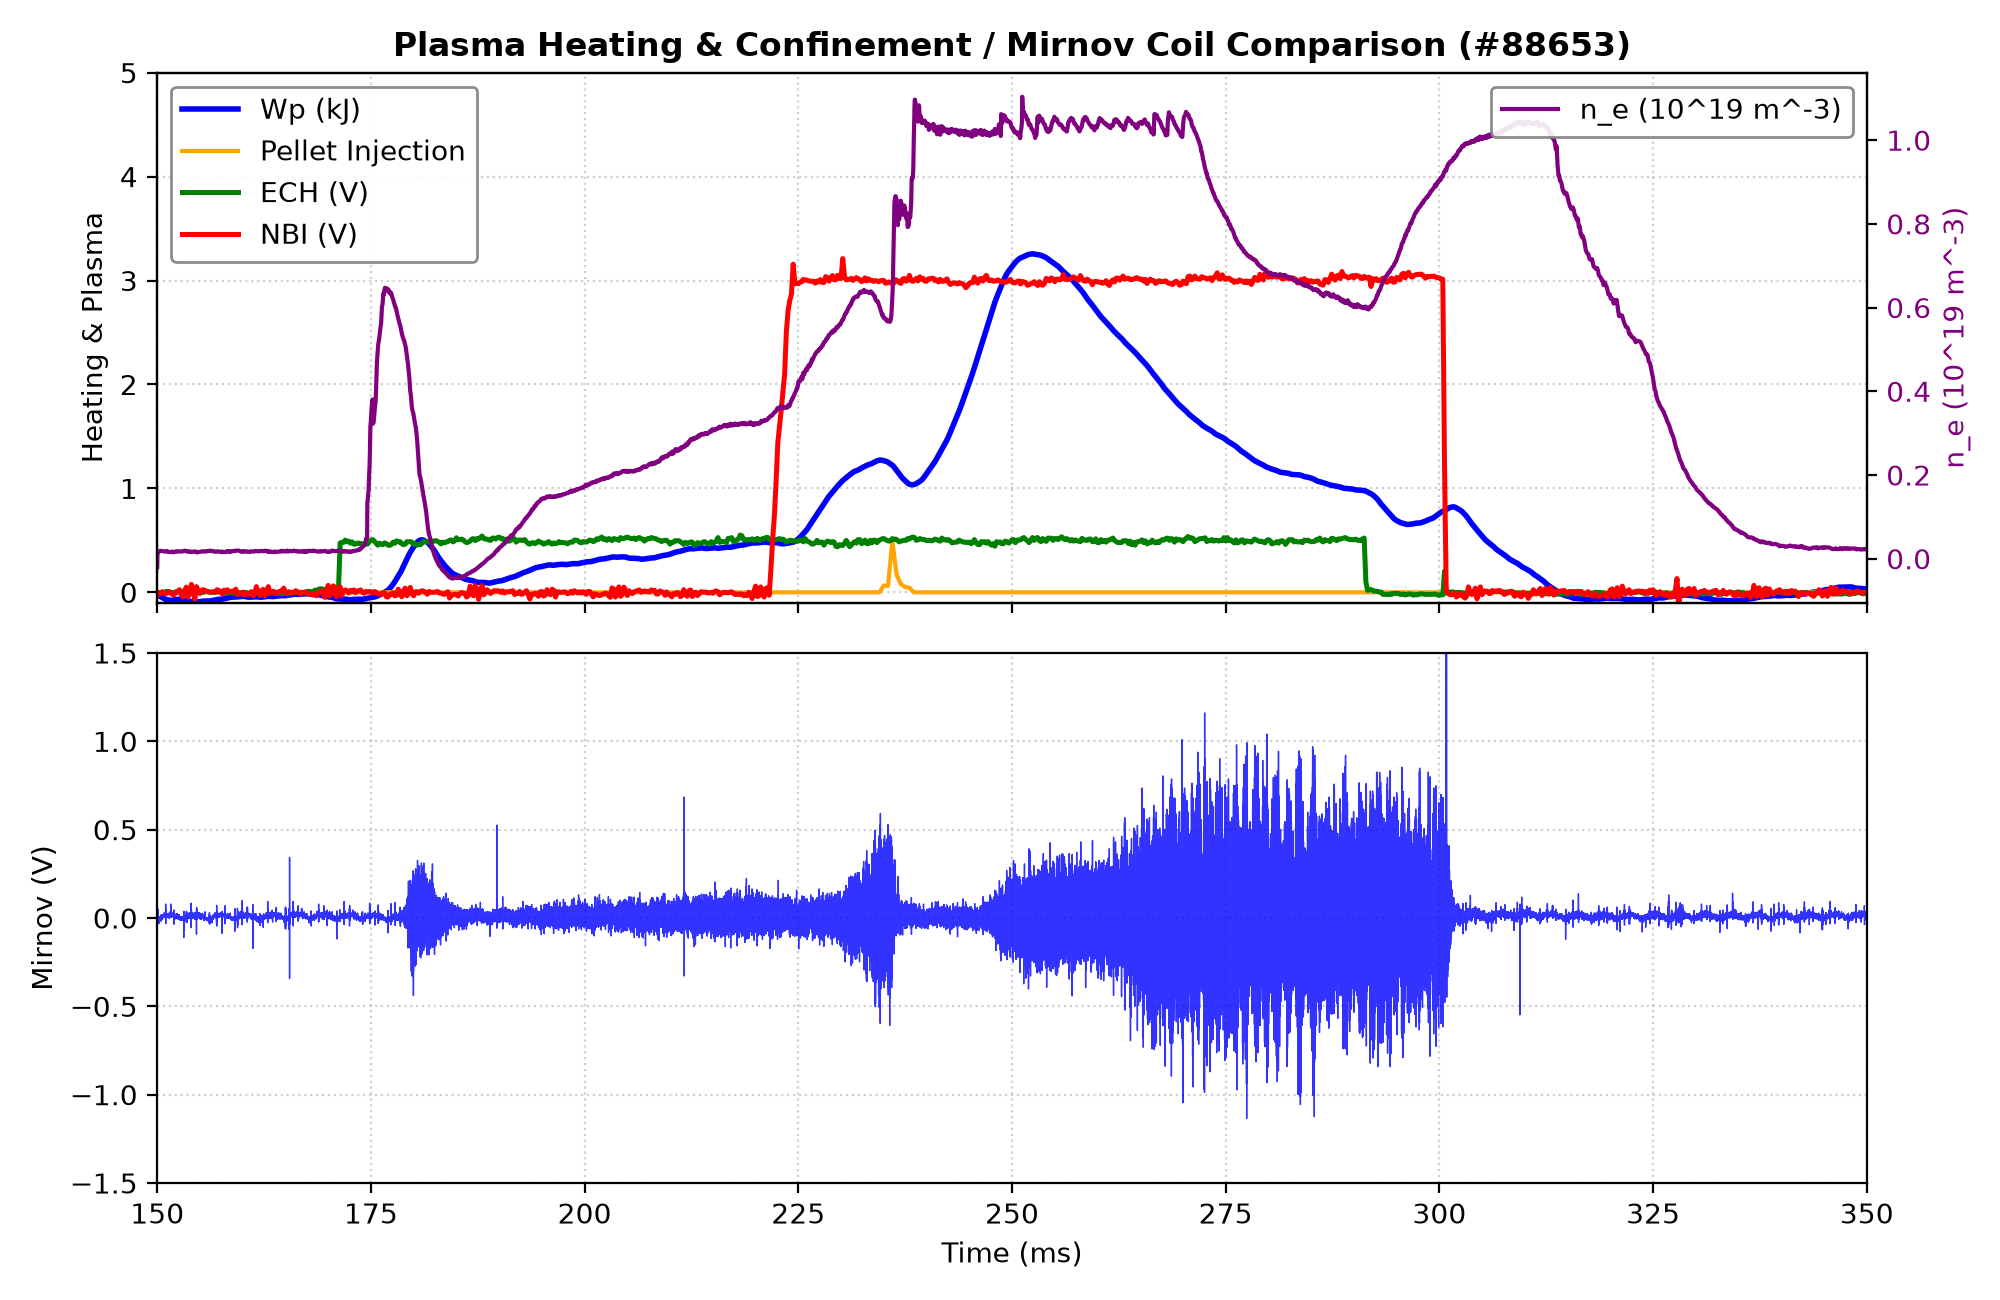
\includegraphics[height=0.81\textheight,keepaspectratio]{Images/obj2_dynamics_and_structure/heating_vs_mirnov (Shot_88653).png}
\end{frame}

\begin{frame}{Overview: Primary and Secondary Modes}
    \centering
    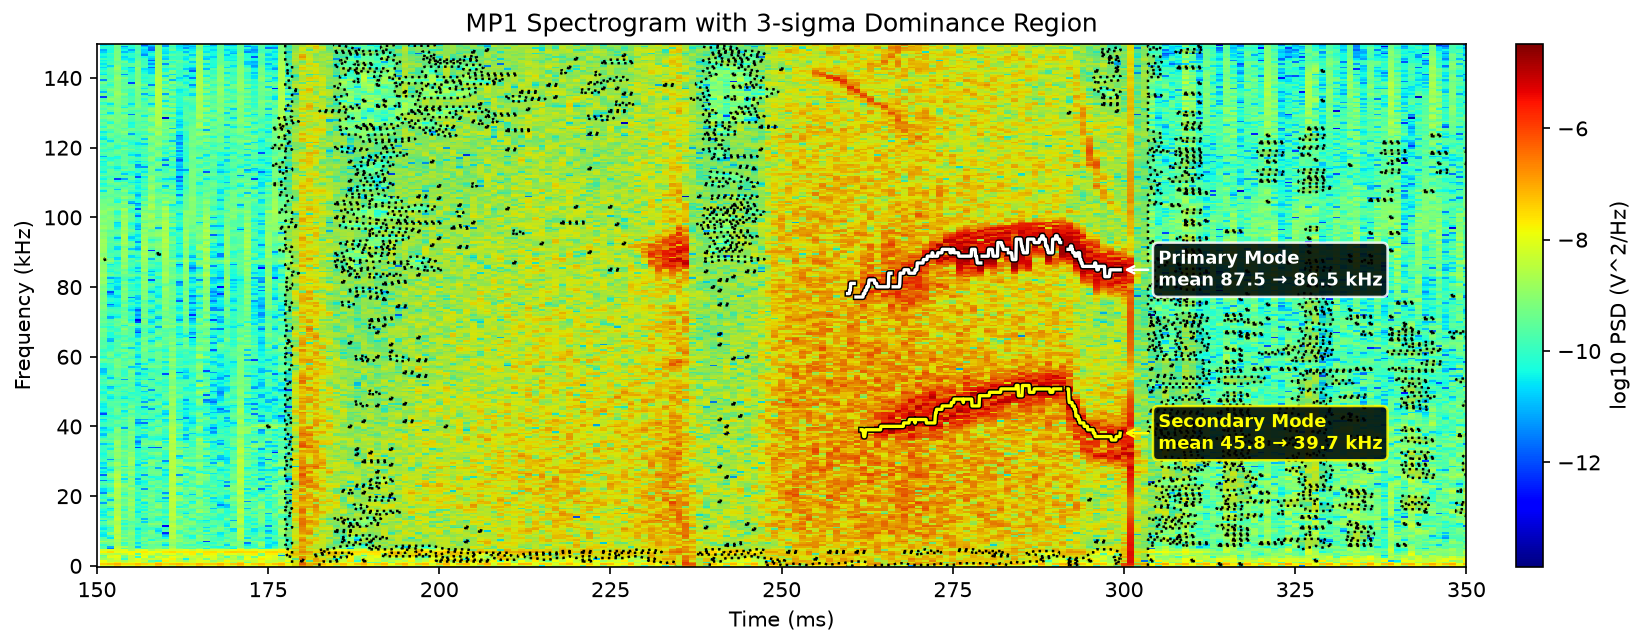
\includegraphics[width=0.94\textwidth,height=0.50\textheight,keepaspectratio]{Images/obj1_mode_identification/panels/mhd_analysis_objective1_88653_panel1_mp1_spectrogram_with_3_sigma_dominance_r.png}
    \vspace{0.1cm}
    \small
    \begin{itemize}
        \item Two coherent modes pass the dual criterion ($3\sigma$ and $\gamma^2>0.7$): \Prim{} (${\sim}\SIrange{80}{100}{kHz}$) and \Sec{} (${\sim}\SIrange{40}{50}{kHz}$).
        \item Both appear with NBI, persist past ECH off (\SI{291.2}{ms}), and disappear when beams stop.
    \end{itemize}
\end{frame}

% ============================================================
\section{Objective 1: Mode Structure \& Dynamics}
% ============================================================

% Reminder of Objective 1 + how it was obtained
\begin{frame}{Specific Objective 1}
    \vfill
    \begin{block}{Spectral properties \& temporal evolution}
        \large Identify the dominant coherent MHD modes, determine their structure
        ($m$, $n$) and follow how they evolve in time -- with and without ECH.
    \end{block}
    \vspace{0.5cm}
    \begin{exampleblock}{How}
        \small MP1 spectrogram + $3\sigma$/$\gamma^2$ gate $\rightarrow$ modes;
        PMP1--14 phase fit $\rightarrow$ $m$; MP1/MP3/MP4 cross-phase fit $\rightarrow$ $n$;
        ridge tracking on zoomed spectrograms $\rightarrow$ dynamics. Run separately on each window.
    \end{exampleblock}
    \vfill
\end{frame}

% Mode structure table: 4 quadrants (columns = windows, rows = modes)
\begin{frame}{Mode Structure}
    \centering
    \renewcommand{\arraystretch}{1.8}
    \setlength{\tabcolsep}{5pt}
    \begin{tabular}{|C{2.8cm}|C{3.3cm}||C{2.8cm}|C{3.3cm}|}
        \hline
        \multicolumn{2}{|c||}{\cellcolor{blue!12}\winA} &
        \multicolumn{2}{c|}{\cellcolor{blue!12}\winB} \\
        \hline
        \cellcolor{red!8}\Prim\newline $f\approx\SI{89}{kHz}$ &
        $m=+3$\newline $n\equiv-1$ (mod 4) &
        \cellcolor{red!8}\Prim\newline $f\approx\SI{86}{kHz}$ &
        $m=+3$\newline $n\equiv-1$ (mod 4) \\
        \hline
        \cellcolor{orange!12}\Sec\newline $f\approx\SI{49}{kHz}$ &
        $m=+6$ \incl\newline $n\equiv-1$ (mod 4) &
        \cellcolor{orange!12}\Sec\newline $f\approx\SI{41}{kHz}$ &
        $m=+2$ \incl\newline $n\equiv-1$ (mod 4) \\
        \hline
    \end{tabular}

    \vspace{0.3cm}
    \footnotesize
    \raggedright
    \begin{itemize}
        \item \Prim: $m=+3$ confirmed in both windows ($r_{\text{circ}}=0.88$, $0.90$);
        \Sec: $m$ jumps $+6\to+2$ with $r_{\text{circ}}=0.22$, $0.63<0.7$.
        \item Both modes share the same toroidal helicity in both windows
        ($\gamma^2\ge0.95$ on all MP pairs); three probes fix $n$ only modulo 4
        ($n\in\{\dots,-5,-1,+3,\dots\}$).
    \end{itemize}
    \vfill
    {\tiny\textsuperscript{*} $f$ = PSD peak used in the fit\par}
\end{frame}

% Poloidal structure: same positions as the table
\begin{frame}{Mode Structure: Poloidal Mode Number $m$}
    \begin{columns}[onlytextwidth,T]
        \begin{column}{0.485\textwidth}
            \colhead{\winA}
            \vspace{0.05cm}
            {\scriptsize\Prim{} (\SI{89.8}{kHz}): $m=+3$}\\[-0.05cm]
            \centering
            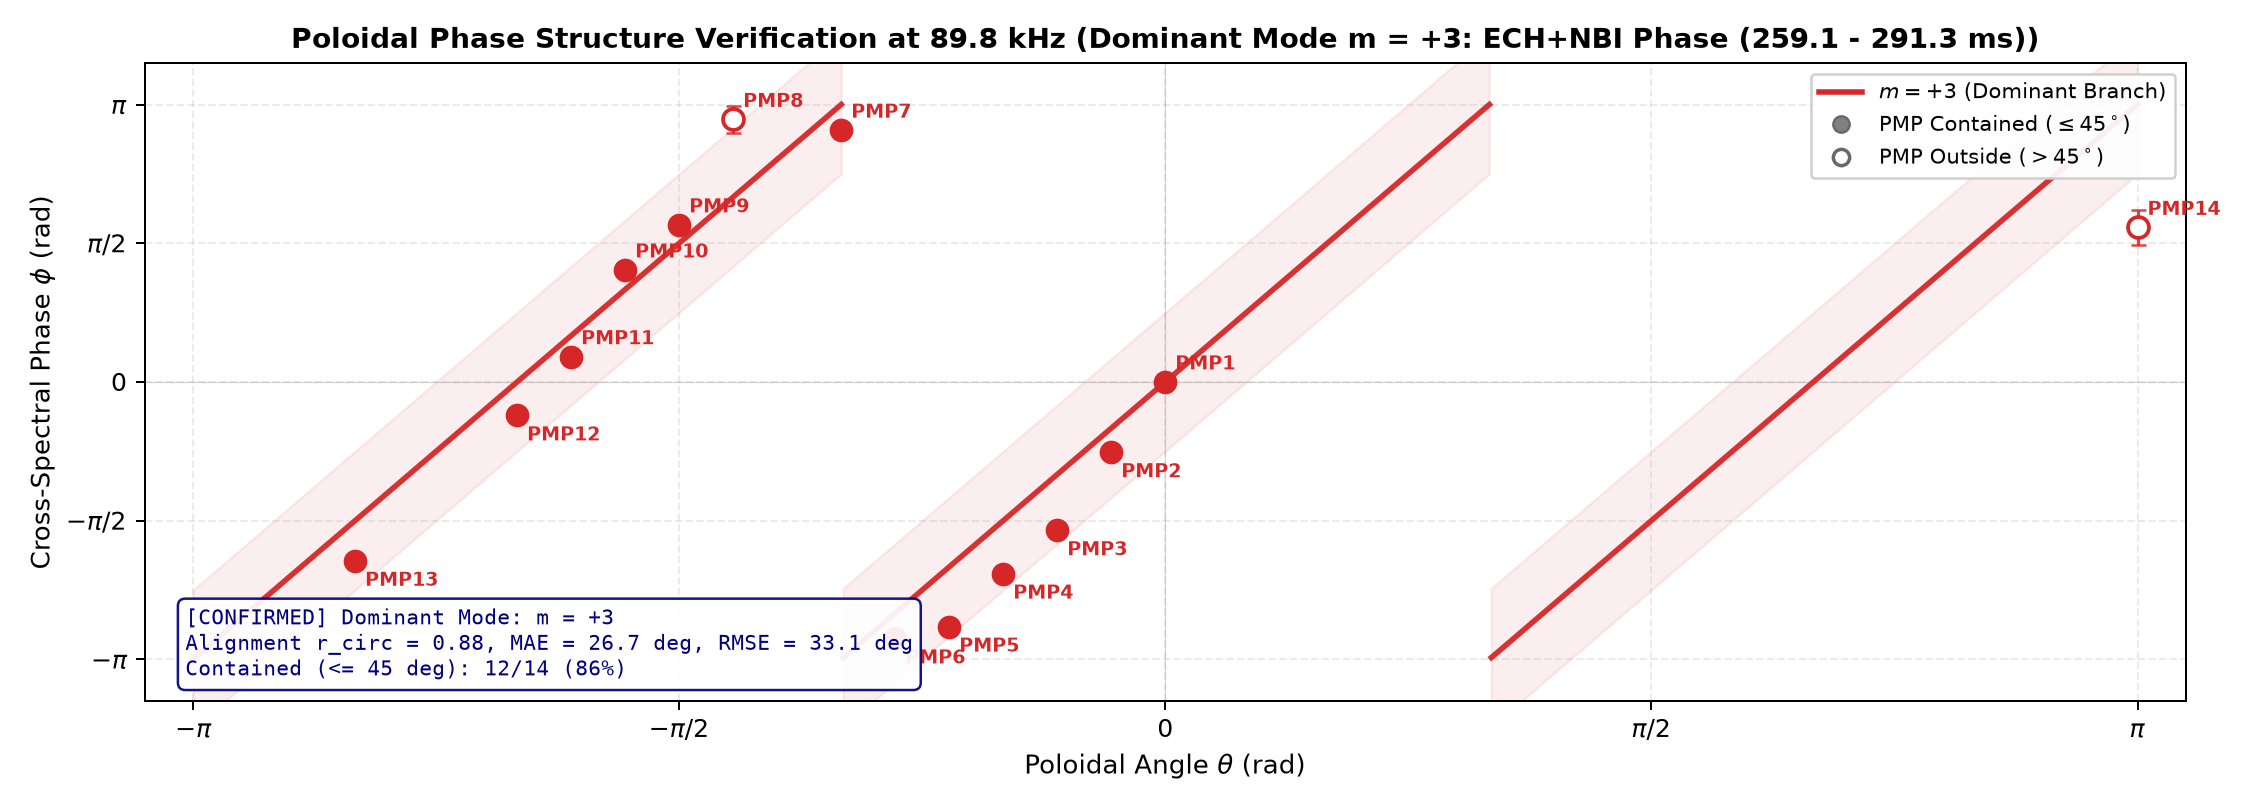
\includegraphics[width=\linewidth,height=0.31\textheight,keepaspectratio]{Images/heating_phase_comparison/panels/mhd_analysis_objective2_structure_88653_80_120kHz_ECH_NBI_panel4_poloidal_phase_structure_verification_at.png}\\
            \raggedright
            {\scriptsize\Sec{} (\SI{48.8}{kHz}): $m=+6$ \incl}\\[-0.05cm]
            \centering
            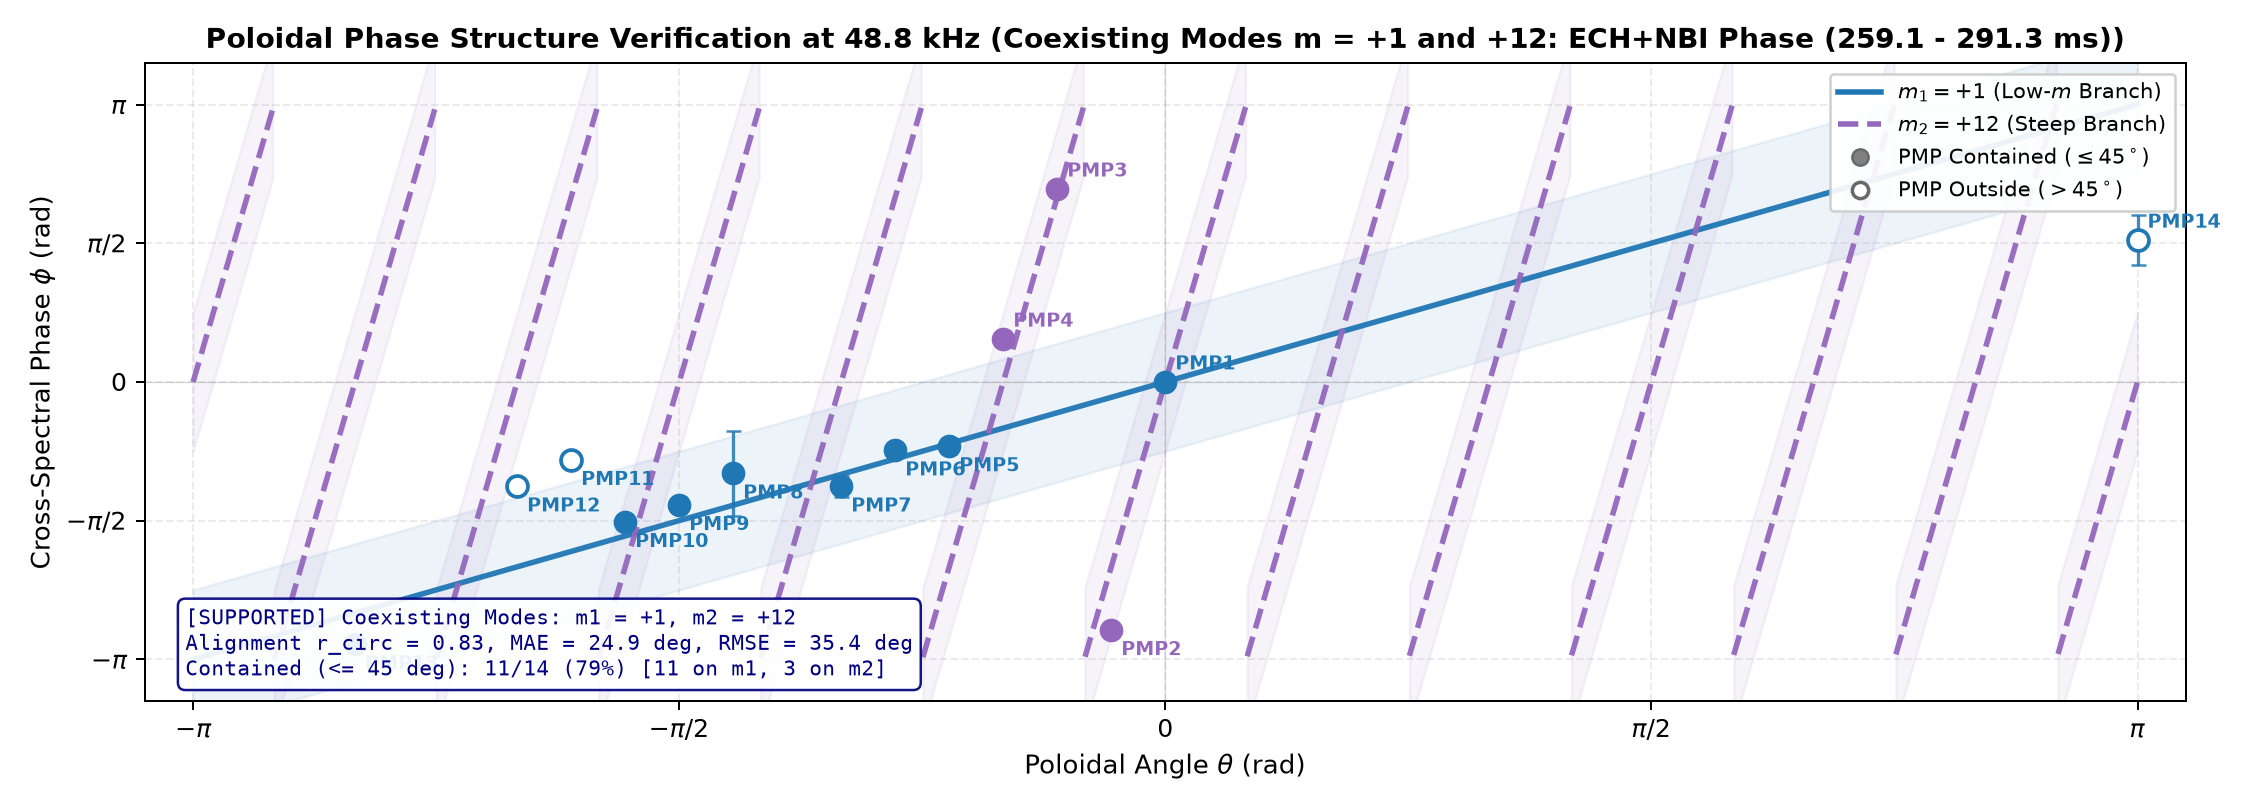
\includegraphics[width=\linewidth,height=0.31\textheight,keepaspectratio]{Images/heating_phase_comparison/panels/mhd_analysis_objective2_structure_88653_40_80kHz_ECH_NBI_panel4_poloidal_phase_structure_verification_at.png}
        \end{column}%
        \hfill
        \begin{column}{0.485\textwidth}
            \colhead{\winB}
            \vspace{0.05cm}
            {\scriptsize\Prim{} (\SI{85.9}{kHz}): $m=+3$}\\[-0.05cm]
            \centering
            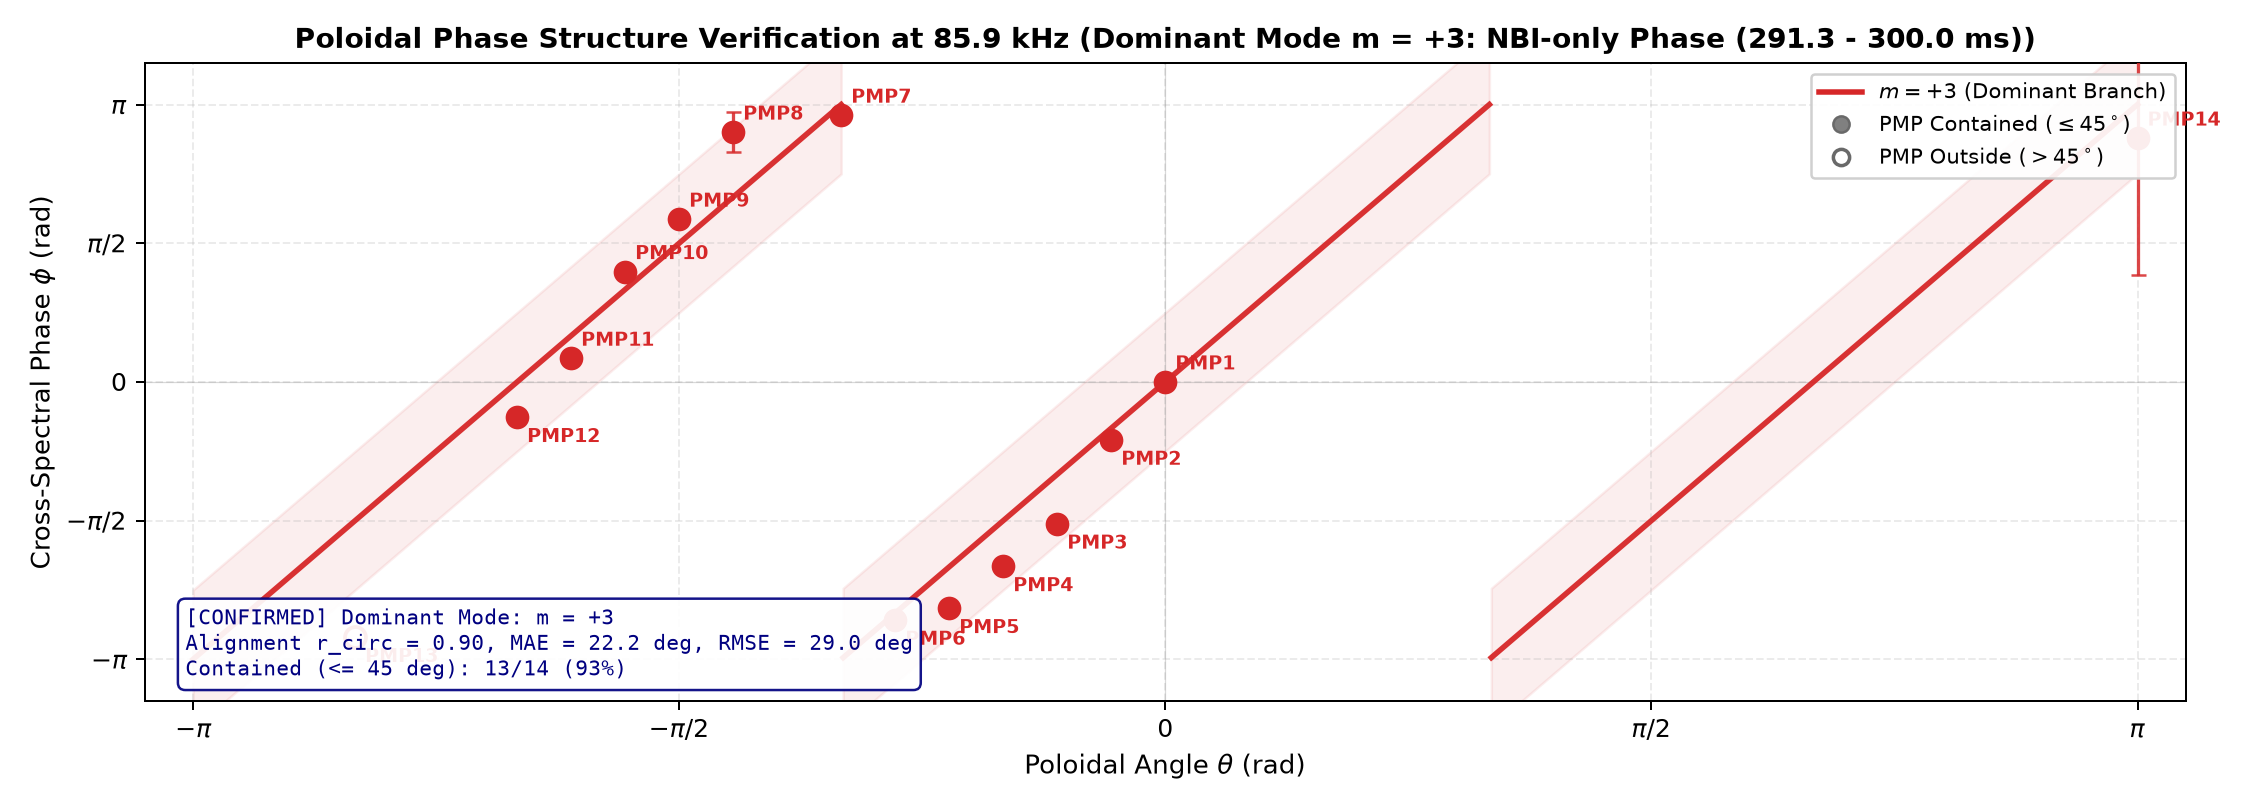
\includegraphics[width=\linewidth,height=0.31\textheight,keepaspectratio]{Images/heating_phase_comparison/panels/mhd_analysis_objective2_structure_88653_80_120kHz_NBI_only_panel4_poloidal_phase_structure_verification_at.png}\\
            \raggedright
            {\scriptsize\Sec{} (\SI{41.0}{kHz}): $m=+2$ \incl}\\[-0.05cm]
            \centering
            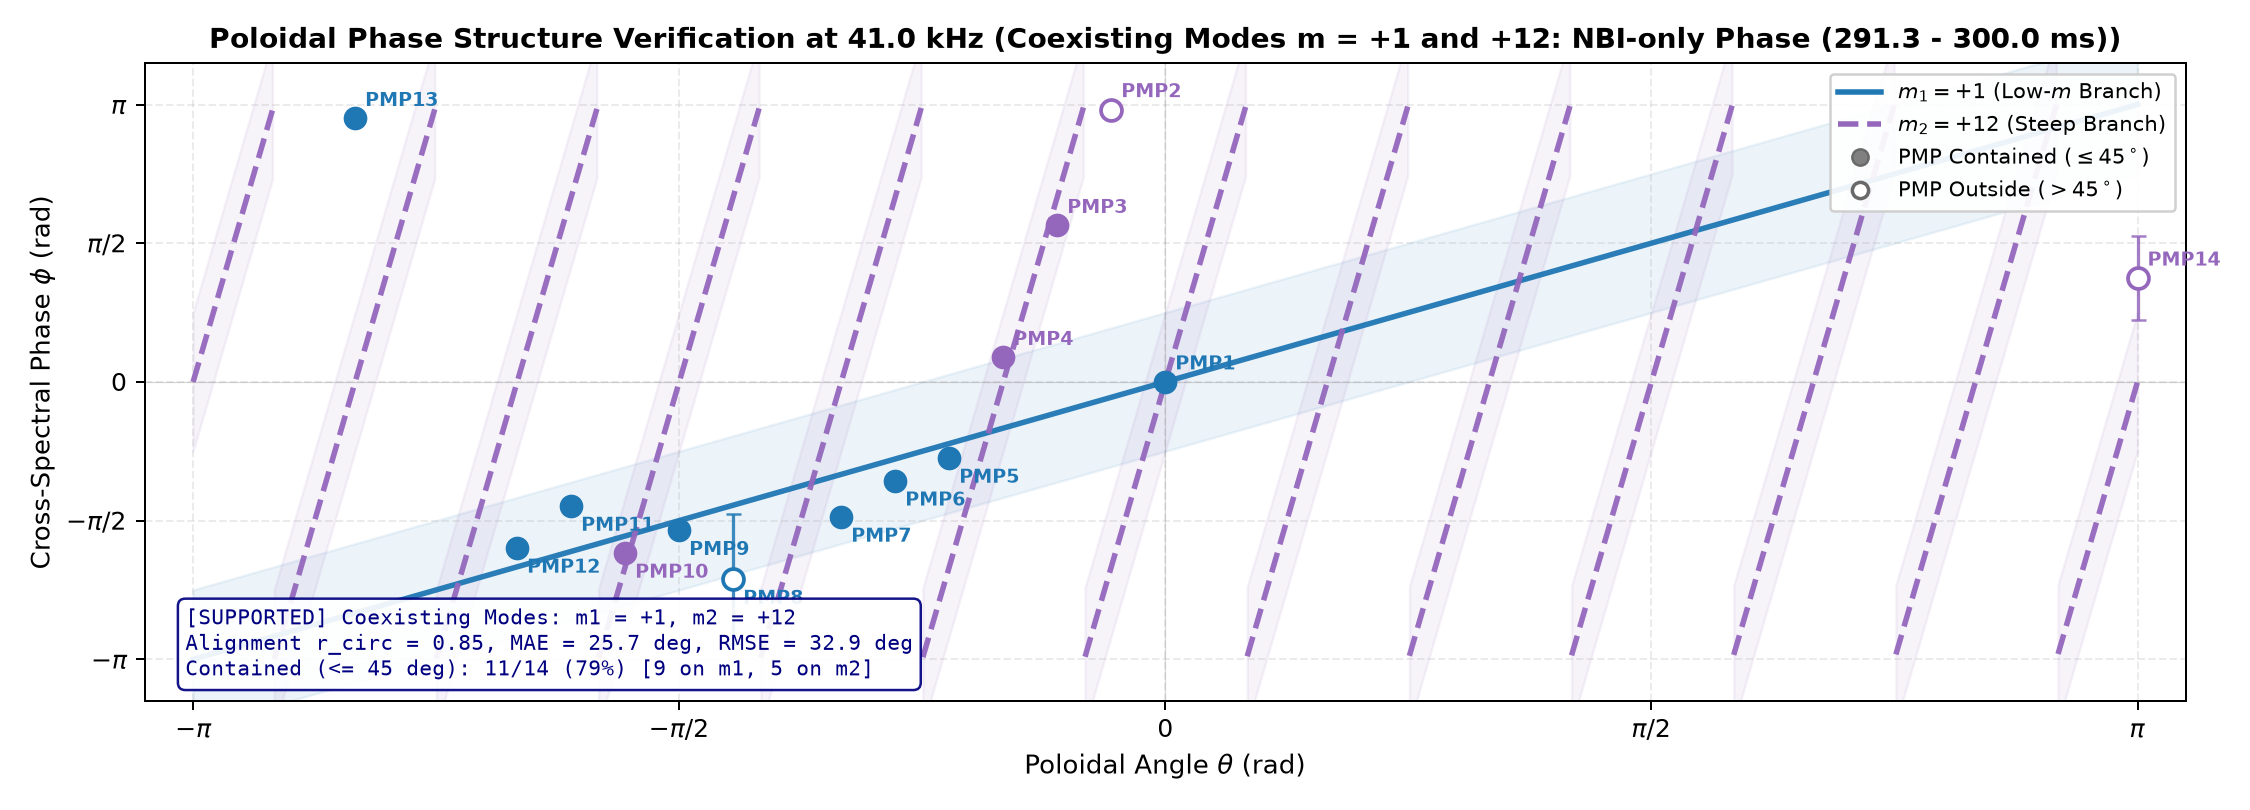
\includegraphics[width=\linewidth,height=0.31\textheight,keepaspectratio]{Images/heating_phase_comparison/panels/mhd_analysis_objective2_structure_88653_40_80kHz_NBI_only_panel4_poloidal_phase_structure_verification_at.png}
        \end{column}
    \end{columns}
    \vfill
    {\tiny\textsuperscript{*} $f$ = PSD peak used in the fit\par}
\end{frame}

% Toroidal structure: same positions as the table
\begin{frame}{Mode Structure: Toroidal Mode Number $n$}
    \begin{columns}[onlytextwidth,T]
        \begin{column}{0.485\textwidth}
            \colhead{\winA}
            \vspace{0.05cm}
            {\scriptsize\Prim{} (\SI{89.0}{kHz}): $n\equiv-1$ (mod 4), RMSE $=\SI{5.2}{\degree}$}\\[-0.05cm]
            \centering
            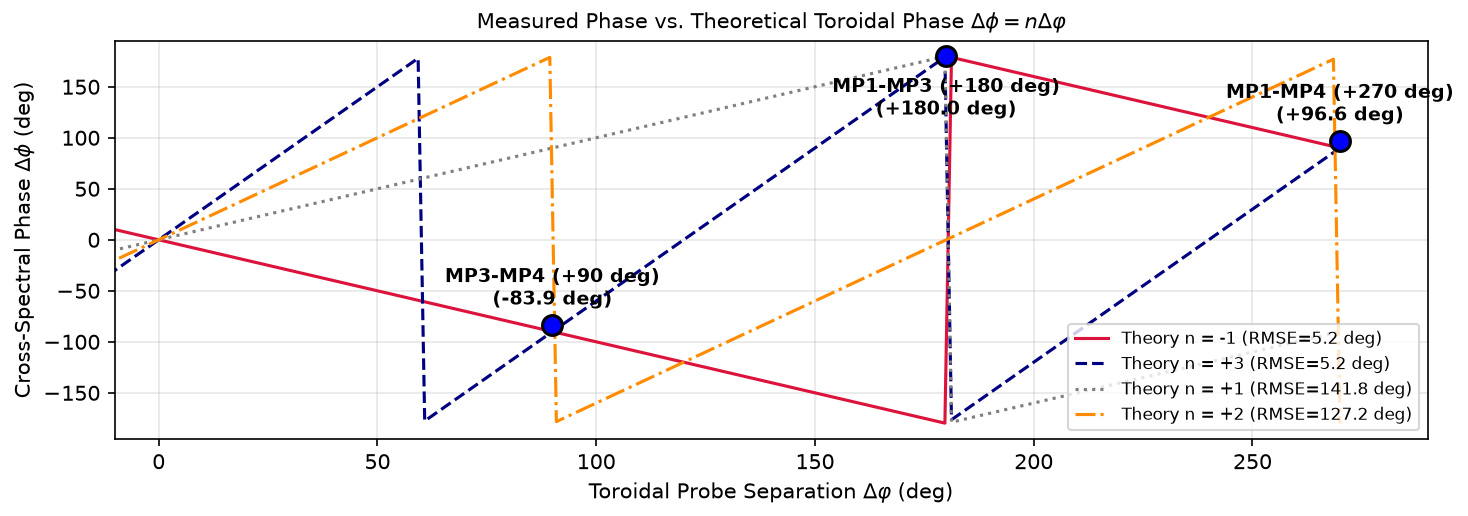
\includegraphics[width=\linewidth,height=0.31\textheight,keepaspectratio]{Images/heating_phase_comparison/panels/mhd_primary_mode_toroidal_n_shot_88653_ECH_NBI_panel2_measured_phase_vs_theoretical_toroidal_p.png}\\
            \raggedright
            {\scriptsize\Sec{} (\SI{48.8}{kHz}): $n\equiv-1$ (mod 4), RMSE $=\SI{22.7}{\degree}$}\\[-0.05cm]
            \centering
            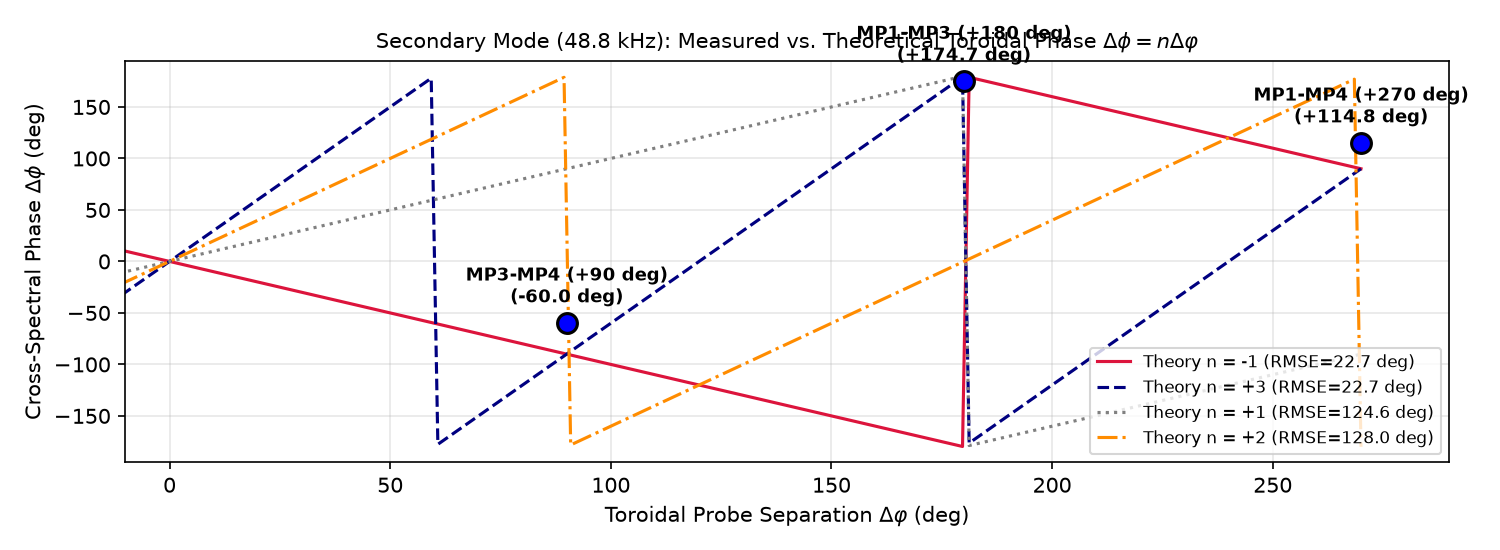
\includegraphics[width=\linewidth,height=0.31\textheight,keepaspectratio]{Images/heating_phase_comparison/panels/mhd_secondary_mode_toroidal_n_shot_88653_ECH_NBI_panel2_measured_phase_vs_theoretical_toroidal_p.png}
        \end{column}%
        \hfill
        \begin{column}{0.485\textwidth}
            \colhead{\winB}
            \vspace{0.05cm}
            {\scriptsize\Prim{} (\SI{86.0}{kHz}): $n\equiv-1$ (mod 4), RMSE $=\SI{6.7}{\degree}$}\\[-0.05cm]
            \centering
            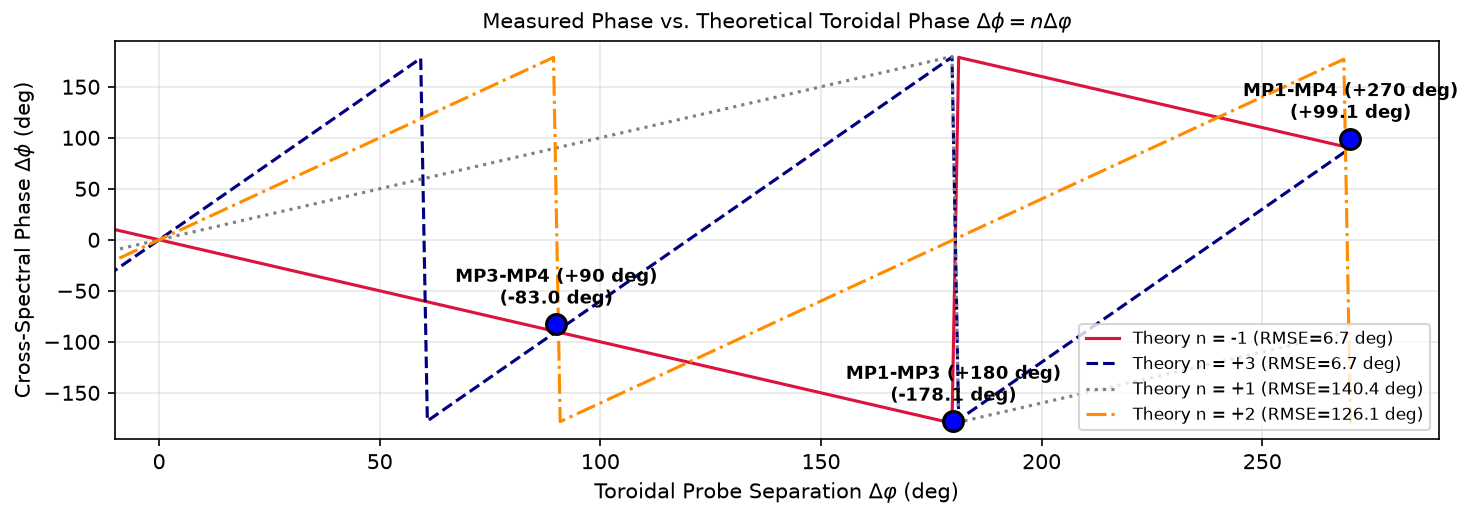
\includegraphics[width=\linewidth,height=0.31\textheight,keepaspectratio]{Images/heating_phase_comparison/panels/mhd_primary_mode_toroidal_n_shot_88653_NBI_only_panel2_measured_phase_vs_theoretical_toroidal_p.png}\\
            \raggedright
            {\scriptsize\Sec{} (\SI{41.0}{kHz}): $n\equiv-1$ (mod 4), RMSE $=\SI{19.3}{\degree}$}\\[-0.05cm]
            \centering
            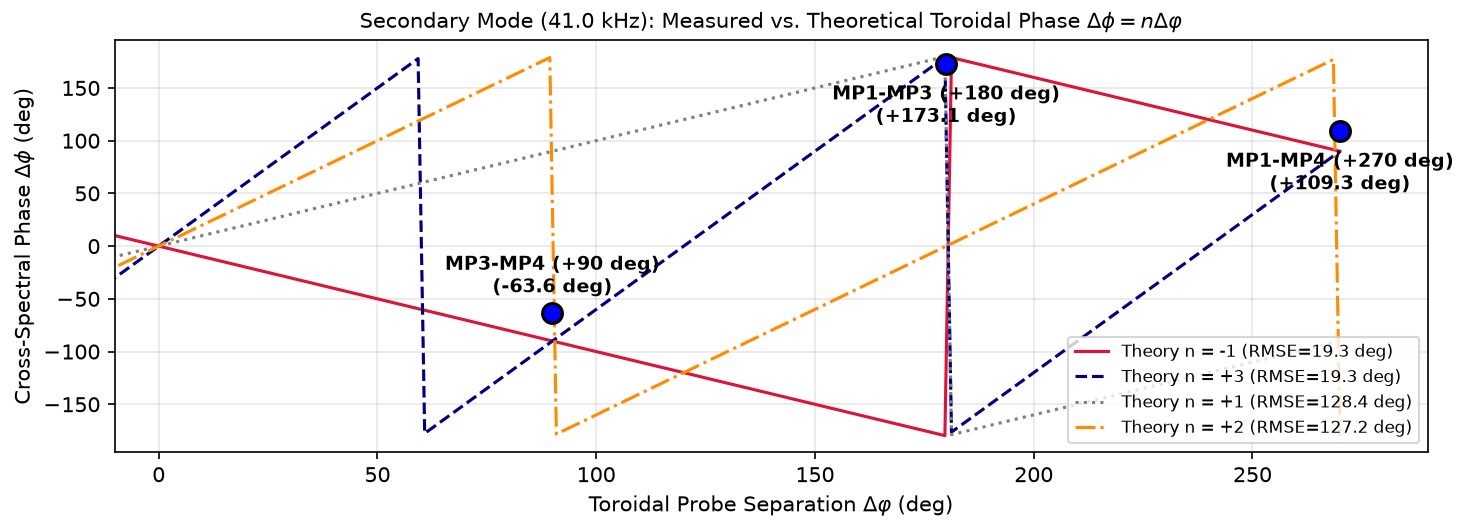
\includegraphics[width=\linewidth,height=0.31\textheight,keepaspectratio]{Images/heating_phase_comparison/panels/mhd_secondary_mode_toroidal_n_shot_88653_NBI_only_panel2_measured_phase_vs_theoretical_toroidal_p.png}
        \end{column}
    \end{columns}
    \vfill
    {\tiny\textsuperscript{*} $f$ = PSD peak used in the fit\par}
\end{frame}

% Dynamic behaviour: 4 quadrants
\begin{frame}{Dynamic Behavior of the Modes}
    % Measure natural box body heights and select maximum
    \savebox{\qboxA}{\qboxmeasure{Primary -- chirping, $f\uparrow$}{%
        \item Repetitive ${\sim}$\SI{1}{ms} frequency sweeps, hopping between 2--3 branches.%
        \item Frequency rises: ${\sim}78\to{\sim}\SI{95}{kHz}$ ($\bar{f}=\SI{87.5}{kHz}$, $\sigma=\SI{4.9}{kHz}$).%
    }}%
    \savebox{\qboxB}{\qboxmeasure{Primary -- chirping, $f\downarrow$}{%
        \item Same chirping and branch-hopping character.%
        \item Frequency falls: ${\sim}90\to{\sim}\SI{85}{kHz}$ ($\bar{f}=\SI{86.5}{kHz}$, $\sigma=\SI{2.3}{kHz}$) -- consistent with electron cooling after ECH off.%
    }}%
    \savebox{\qboxC}{\qboxmeasure{Secondary -- bursting, $f\uparrow$}{%
        \item Bursty, step-like jumps between branches.%
        \item Frequency rises: ${\sim}40\to{\sim}\SI{52}{kHz}$ ($\bar{f}=\SI{45.8}{kHz}$, $\sigma=\SI{4.5}{kHz}$).%
    }}%
    \savebox{\qboxD}{\qboxmeasure{Secondary -- stable, $f\downarrow$}{%
        \item Smoother, more stable frequency line.%
        \item Frequency falls: ${\sim}51\to{\sim}\SI{37}{kHz}$, then stays flat ($\bar{f}=\SI{39.7}{kHz}$, $\sigma=\SI{3.6}{kHz}$).%
    }}%
    \setlength{\qboxbodyH}{\dimexpr\ht\qboxA+\dp\qboxA\relax}%
    \setlength{\tmpH}{\dimexpr\ht\qboxB+\dp\qboxB\relax}%
    \ifdim\tmpH>\qboxbodyH \setlength{\qboxbodyH}{\tmpH}\fi
    \setlength{\tmpH}{\dimexpr\ht\qboxC+\dp\qboxC\relax}%
    \ifdim\tmpH>\qboxbodyH \setlength{\qboxbodyH}{\tmpH}\fi
    \setlength{\tmpH}{\dimexpr\ht\qboxD+\dp\qboxD\relax}%
    \ifdim\tmpH>\qboxbodyH \setlength{\qboxbodyH}{\tmpH}\fi
    \typeout{Dynamic Behavior max box body height: \the\qboxbodyH}%
    \begin{columns}[onlytextwidth,T]
        \begin{column}{\qboxwidth}
            \colhead{\winA}
            \vspace{0.08cm}
            \qbox{Primary -- chirping, $f\uparrow$}{%
                \item Repetitive ${\sim}$\SI{1}{ms} frequency sweeps, hopping between 2--3 branches.%
                \item Frequency rises: ${\sim}78\to{\sim}\SI{95}{kHz}$ ($\bar{f}=\SI{87.5}{kHz}$, $\sigma=\SI{4.9}{kHz}$).%
            }
            \vspace{0.12cm}
            \qbox{Secondary -- bursting, $f\uparrow$}{%
                \item Bursty, step-like jumps between branches.%
                \item Frequency rises: ${\sim}40\to{\sim}\SI{52}{kHz}$ ($\bar{f}=\SI{45.8}{kHz}$, $\sigma=\SI{4.5}{kHz}$).%
            }
        \end{column}%
        \hfill
        \begin{column}{\qboxwidth}
            \colhead{\winB}
            \vspace{0.08cm}
            \qbox{Primary -- chirping, $f\downarrow$}{%
                \item Same chirping and branch-hopping character.%
                \item Frequency falls: ${\sim}90\to{\sim}\SI{85}{kHz}$ ($\bar{f}=\SI{86.5}{kHz}$, $\sigma=\SI{2.3}{kHz}$) -- consistent with electron cooling after ECH off.%
            }
            \vspace{0.12cm}
            \qbox{Secondary -- stable, $f\downarrow$}{%
                \item Smoother, more stable frequency line.%
                \item Frequency falls: ${\sim}51\to{\sim}\SI{37}{kHz}$, then stays flat ($\bar{f}=\SI{39.7}{kHz}$, $\sigma=\SI{3.6}{kHz}$).%
            }
        \end{column}
    \end{columns}
    \vspace{0.08cm}
    {\scriptsize In both windows the modes persist (3$\sigma$ occupancy 100\%); the frequency drift reverses when ECH stops.\par}
    \vfill
    {\tiny\textsuperscript{*} $\bar{f}$ = mean tracked ridge\par}
\end{frame}

\begin{frame}{Dynamic Behavior: Comparative Zoomed Spectrograms}
    \begin{columns}[onlytextwidth,T]
        \begin{column}{0.485\textwidth}
            \colhead{\winA}
            \centering
            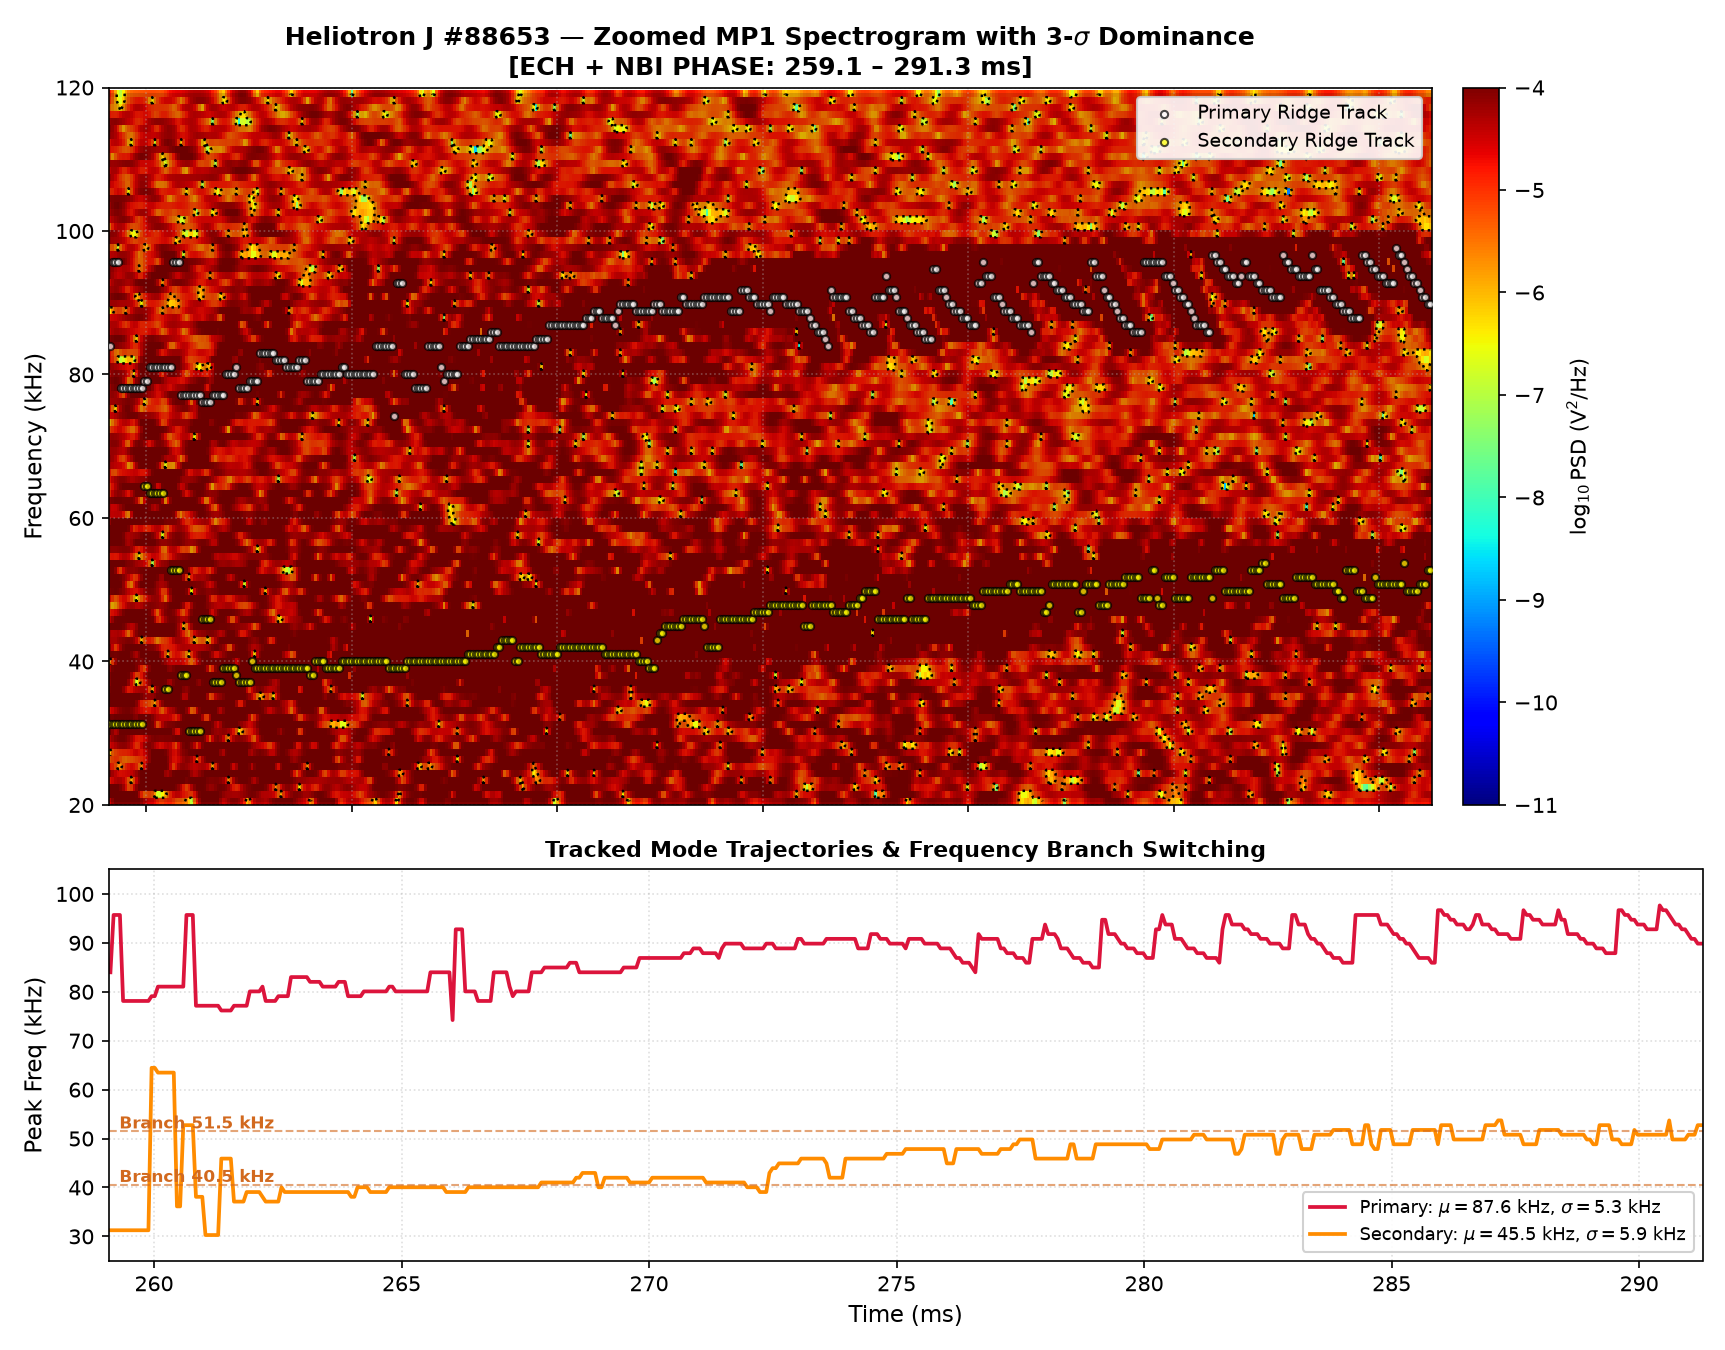
\includegraphics[width=\linewidth,height=0.74\textheight,keepaspectratio]{Images/heating_phase_comparison/zoomed_spectrogram_3sigma_ECH_NBI_259.1_291.3ms.png}
        \end{column}%
        \hfill
        \begin{column}{0.485\textwidth}
            \colhead{\winB}
            \centering
            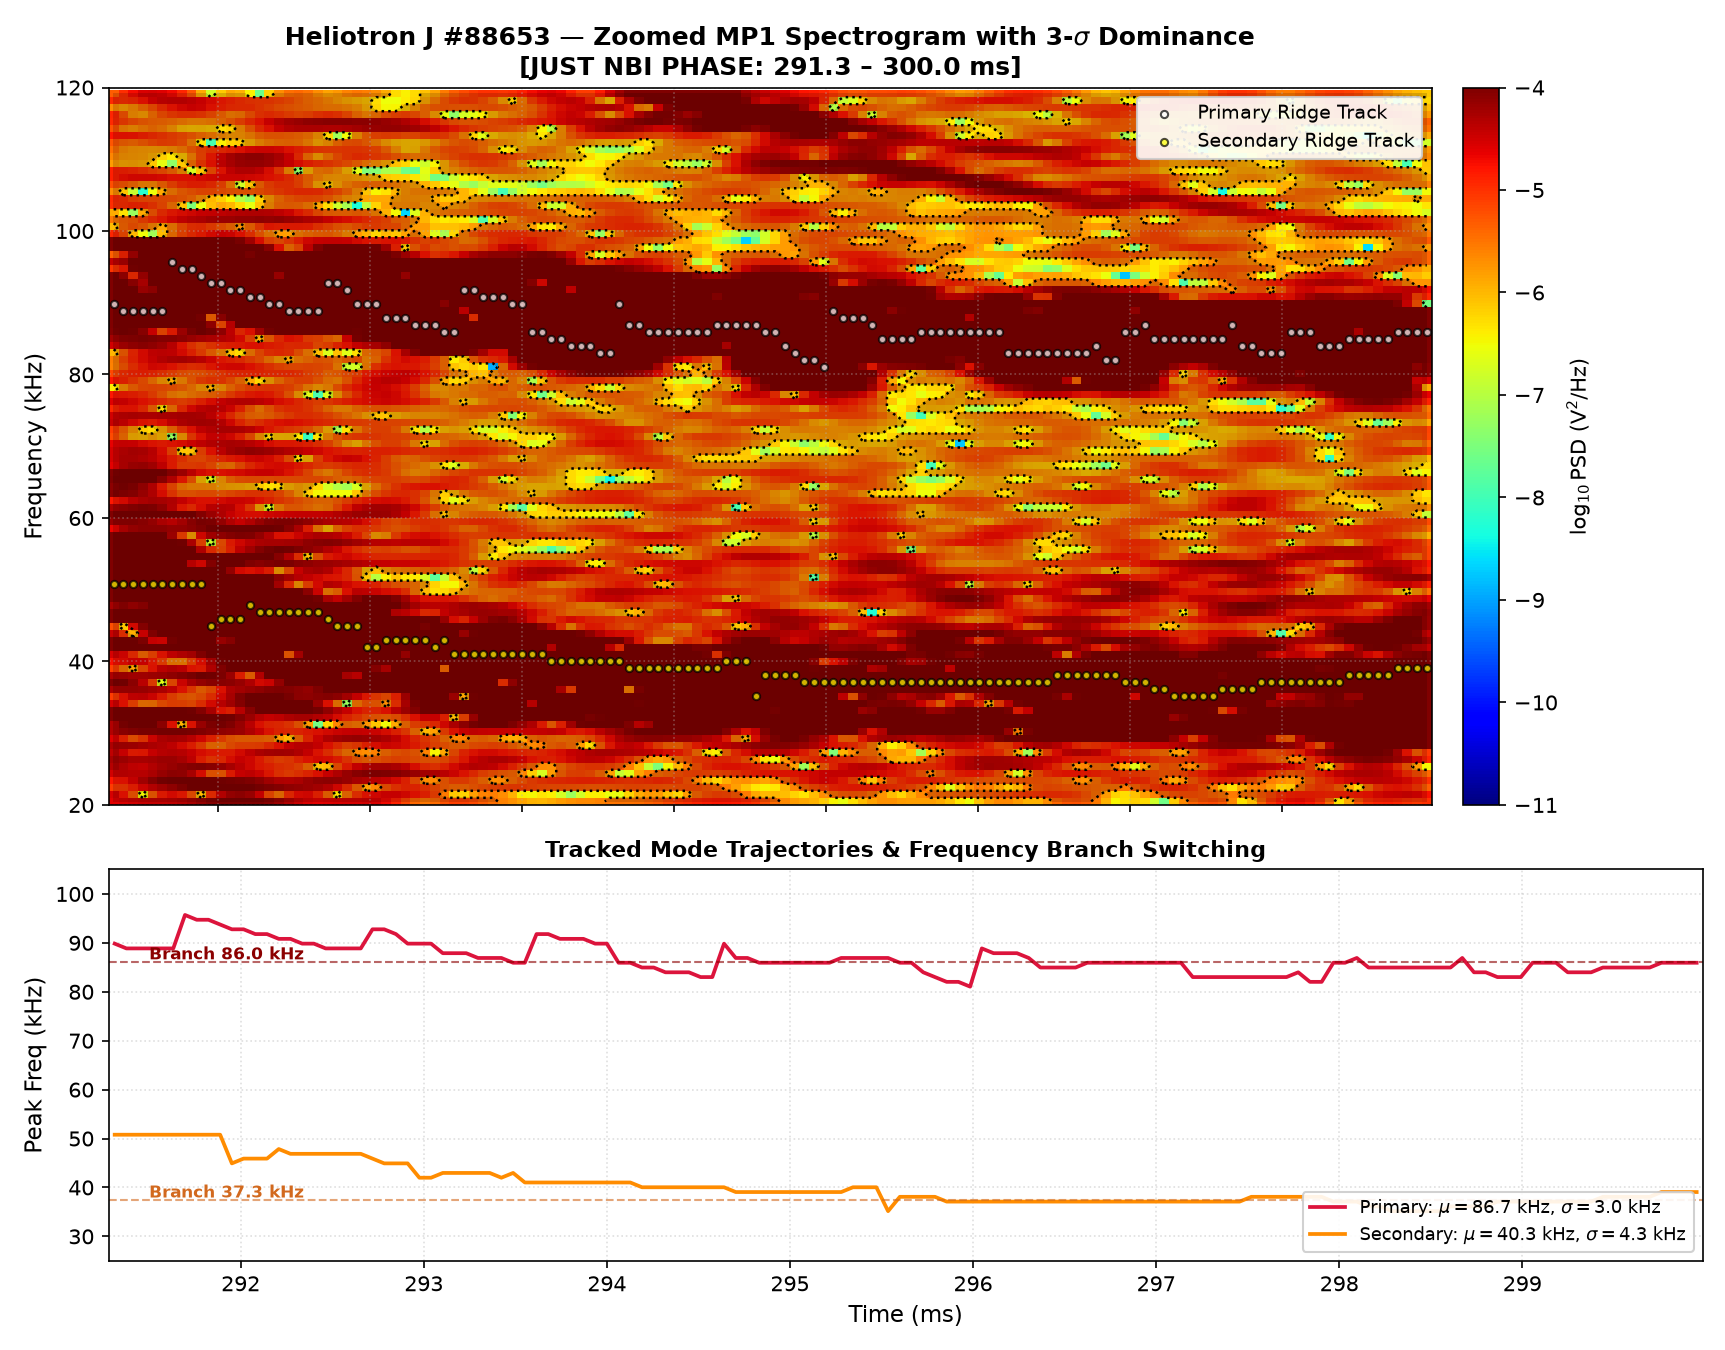
\includegraphics[width=\linewidth,height=0.74\textheight,keepaspectratio]{Images/heating_phase_comparison/zoomed_spectrogram_3sigma_NBI_only_291.3_300.0ms.png}
        \end{column}
    \end{columns}
\end{frame}

% ============================================================
\section{Objective 2: Mode Identification}
% ============================================================

\begin{frame}{Specific Objective 2}
    \vfill
    \begin{block}{EPM--heating correlation}
        \large Link the mode amplitude and frequency to the heating (NBI, ECH) and
        plasma parameters, and test which physical model identifies each mode.
    \end{block}
    \vspace{0.5cm}
    \begin{exampleblock}{How}
        \small Bessel band-pass + Hilbert transform $\rightarrow$ envelope and instantaneous
        frequency of each band; Pearson (with $N_{\text{eff}}$) and partial correlation vs.\
        NBI, ECH, $I_p$, $W_p$, $n_e$, H$\alpha$; frequency compared with six scaling models
        (Alfvénic $1/\sqrt{n_e}$, BAE acoustic $\sqrt{T_e}$, BAE coupled, EPM beam-drive, EPM beam-power, current-induced $I_p$).
    \end{exampleblock}
    \vfill
\end{frame}

\begin{frame}{Mode Identification}
    % Measure natural box body heights and select maximum
    \savebox{\qboxA}{\qboxmeasure{Primary -- BAE/GAM-like (candidate)}{%
        \item Best model (full burst): $f\propto\sqrt{T_e}$ (acoustic / BAE--GAM).%
        \item $r=-0.48$, $p=0.20$ (full burst), opposite sign to prediction \incl%
    }}%
    \savebox{\qboxB}{\qboxmeasure{Primary -- BAE/GAM-like (candidate)}{%
        \item Frequency drops ${\sim}$2--\SI{3}{kHz} (291.3--300.0\,ms): consistent with lower $T_e$.%
        \item Same $m=+3$, same $n$: mode identity preserved without ECH.%
    }}%
    \savebox{\qboxC}{\qboxmeasure{Secondary -- $I_p$-driven (candidate)}{%
        \item Best model (full burst): current-induced ($I_p$, rotational-transform shift).%
        \item $r=-0.85$, $p=0.16$ ($N_{\text{eff}}\approx4$, full burst), opposite sign to prediction \incl%
    }}%
    \savebox{\qboxD}{\qboxmeasure{Secondary -- $I_p$-driven (candidate)}{%
        \item Envelope follows $I_p$ ($r=0.80$) and $W_p$ ($r=0.81$) (291.3--300.0\,ms).%
        \item Frequency shifts downward ($\bar{f}=\SI{39.7}{kHz}$); structure ($m$) unresolved.%
    }}%
    \setlength{\qboxbodyH}{\dimexpr\ht\qboxA+\dp\qboxA\relax}%
    \setlength{\tmpH}{\dimexpr\ht\qboxB+\dp\qboxB\relax}%
    \ifdim\tmpH>\qboxbodyH \setlength{\qboxbodyH}{\tmpH}\fi
    \setlength{\tmpH}{\dimexpr\ht\qboxC+\dp\qboxC\relax}%
    \ifdim\tmpH>\qboxbodyH \setlength{\qboxbodyH}{\tmpH}\fi
    \setlength{\tmpH}{\dimexpr\ht\qboxD+\dp\qboxD\relax}%
    \ifdim\tmpH>\qboxbodyH \setlength{\qboxbodyH}{\tmpH}\fi
    \typeout{Mode Identification max box body height: \the\qboxbodyH}%
    \begin{columns}[onlytextwidth,T]
        \begin{column}{\qboxwidth}
            \colhead{\winA}
            \vspace{0.04cm}
            \qbox{Primary -- BAE/GAM-like (candidate)}{%
                \item Best model (full burst): $f\propto\sqrt{T_e}$ (acoustic / BAE--GAM).%
                \item $r=-0.48$, $p=0.20$ (full burst), opposite sign to prediction \incl%
            }
            \vspace{0.08cm}
            \qbox{Secondary -- $I_p$-driven (candidate)}{%
                \item Best model (full burst): current-induced ($I_p$, rotational-transform shift).%
                \item $r=-0.85$, $p=0.16$ ($N_{\text{eff}}\approx4$, full burst), opposite sign to prediction \incl%
            }
        \end{column}%
        \hfill
        \begin{column}{\qboxwidth}
            \colhead{\winB}
            \vspace{0.04cm}
            \qbox{Primary -- BAE/GAM-like (candidate)}{%
                \item Frequency drops ${\sim}$2--\SI{3}{kHz} (291.3--300.0\,ms): consistent with lower $T_e$.%
                \item Same $m=+3$, same $n$: mode identity preserved without ECH.%
            }
            \vspace{0.08cm}
            \qbox{Secondary -- $I_p$-driven (candidate)}{%
                \item Envelope follows $I_p$ ($r=0.80$) and $W_p$ ($r=0.81$) (291.3--300.0\,ms).%
                \item Frequency shifts downward ($\bar{f}=\SI{39.7}{kHz}$); structure ($m$) unresolved.%
            }
        \end{column}
    \end{columns}
    \vspace{0.04cm}
    {\scriptsize Drive: once the ECH on/off step is partialled out, $r_{\text{ECH}}\to0.06$--$0.12$
    while $r_{\text{NBI}}\approx0.61$--$0.64$ survives $\Rightarrow$ NBI fast ions drive both modes.
    No scaling model is significant (adjusted $p>0.16$); tests use the full active burst.\par}
\end{frame}

% ============================================================
\section{Objective 3: Non-linear Coupling}
% ============================================================

\begin{frame}{Specific Objective 3}
    \vfill
    \begin{block}{Low-frequency H-mode fluctuations \& edge coupling}
        \large Find out whether the modes exchange energy through three-wave
        (non-linear) coupling, and whether this is linked to edge turbulence and heat transport.
    \end{block}
    \vspace{0.5cm}
    \begin{exampleblock}{How}
        \small Squared auto-bicoherence of MP1 ($N_{\text{ens}}=30$) in each window, computed with a corrected estimator;
        significance from an amplitude-conditioned surrogate null (family-wise $p$-values);
        replication check in shot \#88654.
    \end{exampleblock}
    \vfill
\end{frame}

\begin{frame}{Bicoherence Analysis}
    \begin{columns}[onlytextwidth,T]
        \begin{column}{0.485\textwidth}
            \colhead{\textbf{NBI + ECH}\\[-0.2ex]{\scriptsize(\SIrange{259.1}{267.0}{ms}, $N_{\text{fft}}=512$, $N_{\text{ens}}=30$)}}
            \vspace{0.04cm}
            \footnotesize
            \begin{itemize}
                \item Max $b^2=0.335$ in the search domain ($f_1,|f_2|\le\SI{100}{kHz}$) at $76.2+72.3=\SI{148.4}{kHz}$; family-wise $p\approx0.42$--$0.43$ (3 seeds $\times$ 5000 surrogates).
                \item Carried by a short burst at \SIrange{265}{267}{ms}; the same triad in shot \#88654 gives $b^2=0.378$ (per-bin $p=0.026$).
            \end{itemize}
        \end{column}%
        \hfill
        \begin{column}{0.485\textwidth}
            \colhead{\textbf{NBI only}\\[-0.2ex]{\scriptsize(\SIrange{291.3}{299.2}{ms}, $N_{\text{fft}}=512$, $N_{\text{ens}}=30$)}}
            \vspace{0.04cm}
            \footnotesize
            \begin{itemize}
                \item Max $b^2=0.712$ in the search domain ($f_1,|f_2|\le\SI{100}{kHz}$) at $74.2+23.4=\SI{97.7}{kHz}$; family-wise $p\approx0.06$.
                \item 71\% of $|z|$ comes from one segment at \SI{291.6}{ms} (0.4\,ms after ECH-off); $b^2=0.37$ without it; not reproduced in shot \#88654 ($b^2=0.083$).
            \end{itemize}
        \end{column}
    \end{columns}
    \vspace{0.06cm}
    \begin{alertblock}{Control windows}
        \footnotesize Both maxima lie within the spread of the maxima of 33 non-overlapping control windows per shot (see backup; median 0.42 and 0.50; 3 and 8 of 33 windows reach 0.71); no triad is distinguishable from the null. Peaks on the self-product line also occur in control windows (mean 2.7 and 2.2 of 10 per shot): 6 of 10 on the ECH+NBI map is reached or exceeded by 2 of 66 control windows, 3 of 10 on the NBI-only map by 33 of 66.
    \end{alertblock}
\end{frame}

\begin{frame}{Bicoherence Maps}
    \begin{columns}[onlytextwidth,T]
        \begin{column}{0.485\textwidth}
            \colhead{\textbf{NBI + ECH}\\[-0.2ex]{\scriptsize(\SIrange{259.1}{267.0}{ms})}}
            \centering
            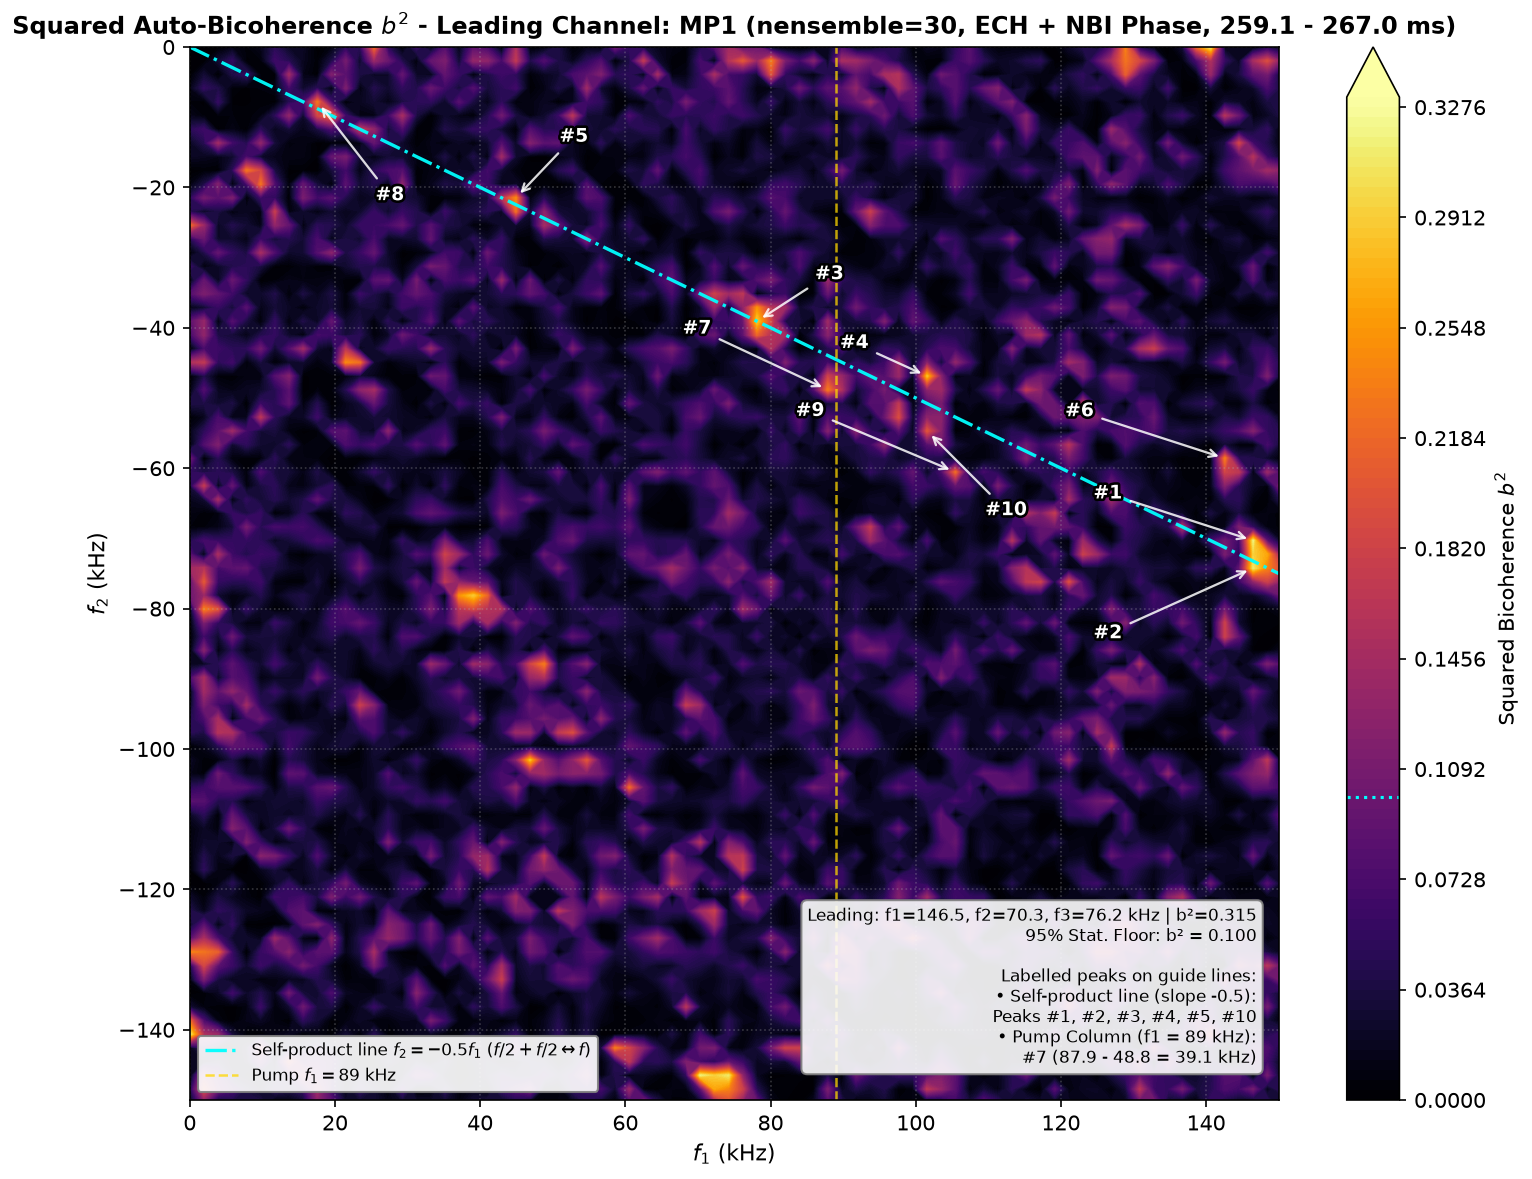
\includegraphics[width=\linewidth,height=0.58\textheight,keepaspectratio]{Images/obj3_nonlinear_coupling/corrected_bicoherence_map_ECH_NBI.png}
        \end{column}%
        \hfill
        \begin{column}{0.485\textwidth}
            \colhead{\textbf{NBI only}\\[-0.2ex]{\scriptsize(\SIrange{291.3}{299.2}{ms})}}
            \centering
            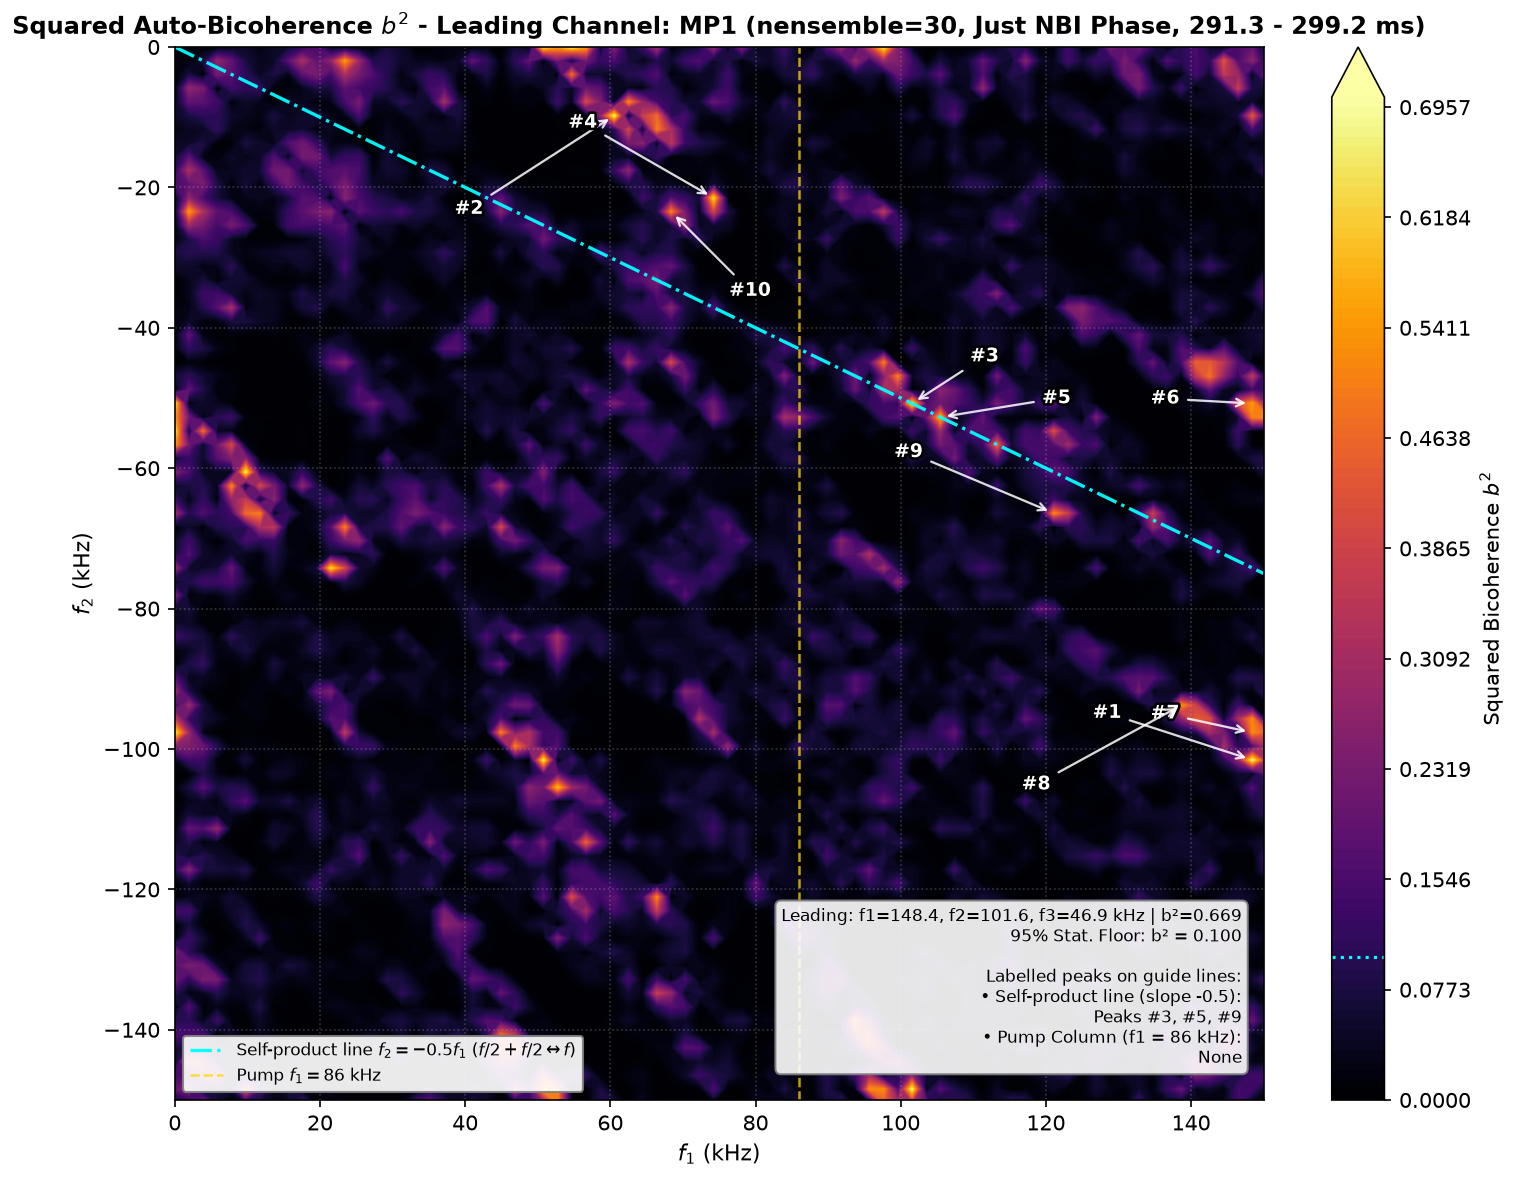
\includegraphics[width=\linewidth,height=0.58\textheight,keepaspectratio]{Images/obj3_nonlinear_coupling/corrected_bicoherence_map_NBI_only.png}
        \end{column}
    \end{columns}
    \vspace{0.05cm}

    {\scriptsize Dash-dot line: $f_2=-f_1/2$ (self-product triads $f/2+f/2\leftrightarrow f$); arrows: ten largest local maxima, $f_1\le\SI{150}{kHz}$; badge $b^2$ is the maximum of this difference-form map, not of the search domain.\par}
\end{frame}

% ============================================================
\section{Discussion}
% ============================================================

\begin{frame}{Discussion: Objective 1 -- Mode Structure \& Dynamics}
    \begin{itemize}[<+->]
        \item Both modes are coherent ($\gamma^2\ge0.95$ on all MP pairs) and \textbf{survive the ECH shut-off}
        with the same toroidal helicity ($n\equiv-1$ mod 4).
        \item The \Prim{} mode has a robust global structure ($m=+3$ in both windows); the
        \Sec{} mode's $m$ is unstable ($+6\to+2$) $\Rightarrow$ inconclusive.
        \item ECH only sets the \textbf{direction of the frequency drift}: up with ECH,
        down after ECH off (electron cooling).
        \item Chirping and branch hopping (${\sim}$0.4--1.3 jumps/ms) are the hallmark of
        fast-ion-driven (EPM-like) dynamics.
        \item Same modes reappear in shot \#88654, downshifted 1--\SI{2.5}{kHz}.
    \end{itemize}
\end{frame}

\begin{frame}{Discussion: Objective 2 -- Mode Identification}
    \begin{itemize}[<+->]
        \item Mode envelopes track $I_p$, $W_p$ and $n_e$ strongly ($r=0.76$--$0.87$) in both bands.
        \item With the ECH step removed, the ECH correlation vanishes while NBI's survives
        $\Rightarrow$ the modes are \textbf{driven by NBI fast ions}, not by ECH.
        \item Candidate identities: \Prim{} $\rightarrow$ BAE/GAM-like ($\sqrt{T_e}$),
        \Sec{} $\rightarrow$ $I_p$-driven.
        \item But no scaling model is statistically significant ($p>0.16$, $N_{\text{eff}}\approx4$--9,
        opposite signs) $\Rightarrow$ identification remains \textbf{tentative}.
        \item Needed: $T_e$ profiles / equilibrium (Alfvén continuum) and more shots.
    \end{itemize}
\end{frame}

\begin{frame}{Discussion: Objective 3 -- Non-linear Coupling}
    \small
    \begin{itemize}[<+->]
        \item A one-bin offset in the lab bicoherence routine was found and corrected; the headline statistics were recomputed with the corrected estimator.
        \item $259.1$--$275.0$\,ms: no triad is distinguishable from the amplitude-conditioned null (max-$b^2$ $p\approx0.12$--$0.13$; max phase-coherence $p=0.65$).
        \item Heated-window maxima ($0.34$/$0.71$ in 88653, $0.40$/$0.73$ in 88654) lie within the spread of 33 control windows per shot (median $0.42$/$0.50$).
        \item The highest $b^2$ values are carried by a few segments ($N_{\text{eff}}=1$--$5$ of 30): ECH-off and NBI-off transients, and a \SIrange{265}{267}{ms} burst at \SI{148}{kHz} seen on MP1, MP3 and MP4 in both shots.
        \item The self-product $89.8+89.8\to\SI{179.7}{kHz}$ has no stable biphase ($R^2\le0.12$) and its power does not follow the fourth power of the primary (log-log slope $0.2$--$0.4$, not $2$).
        \item Integrated bicoherence is not distinguishable from a calibrated Gaussian null ($p\approx0.10$--$0.15$).
        \item Energy-transfer direction cannot be inferred from single-point bispectra; earlier sign claims are withdrawn.
        \item No evidence for three-wave coupling; no link to turbulence or heat transport is claimed.
    \end{itemize}
\end{frame}

% ============================================================
\section{Summary}
% ============================================================

\begin{frame}{Summary}
    \footnotesize
    \begin{itemize}
        \item Two coherent modes -- \Prim{} ($m=+3$) and \Sec{} ($m$ tentative) -- persist after ECH turns off.
        \vspace{0.2cm}
        \item Both follow NBI; ECH shifts their frequency (up with ECH, down after).
        \vspace{0.2cm}
        \item Non-linear coupling: present, not yet validated.
    \end{itemize}
    \vspace{0.6cm}
    \begin{beamercolorbox}[wd=\textwidth,sep=10pt,center,rounded=true,shadow=true]{block title}
        \large\bfseries In shot \#88653, NBI fast ions sustain the MHD modes;\\
        ECH mainly tunes their frequency.
    \end{beamercolorbox}
\end{frame}

% Thank you / Questions
\begin{frame}
    \begin{center}
        {\Huge Thank you}\\[0.5cm]
        {\Large Questions?}
    \end{center}
\end{frame}

% ================================================================
% ================================================================
%                        BACKUP SLIDES
% ================================================================
% ================================================================
\appendix
\section{Backup Slides}

\begin{frame}
    \begin{center}
        {\usebeamerfont{title}\structure{\Huge Backup Slides}}
    \end{center}
\end{frame}

\subsection{Backup: Objective 1}

\begin{frame}{Backup: Objective 1 -- Spectrogram and Spatial Coherence}
    \begin{figure}[h!]
        \centering
        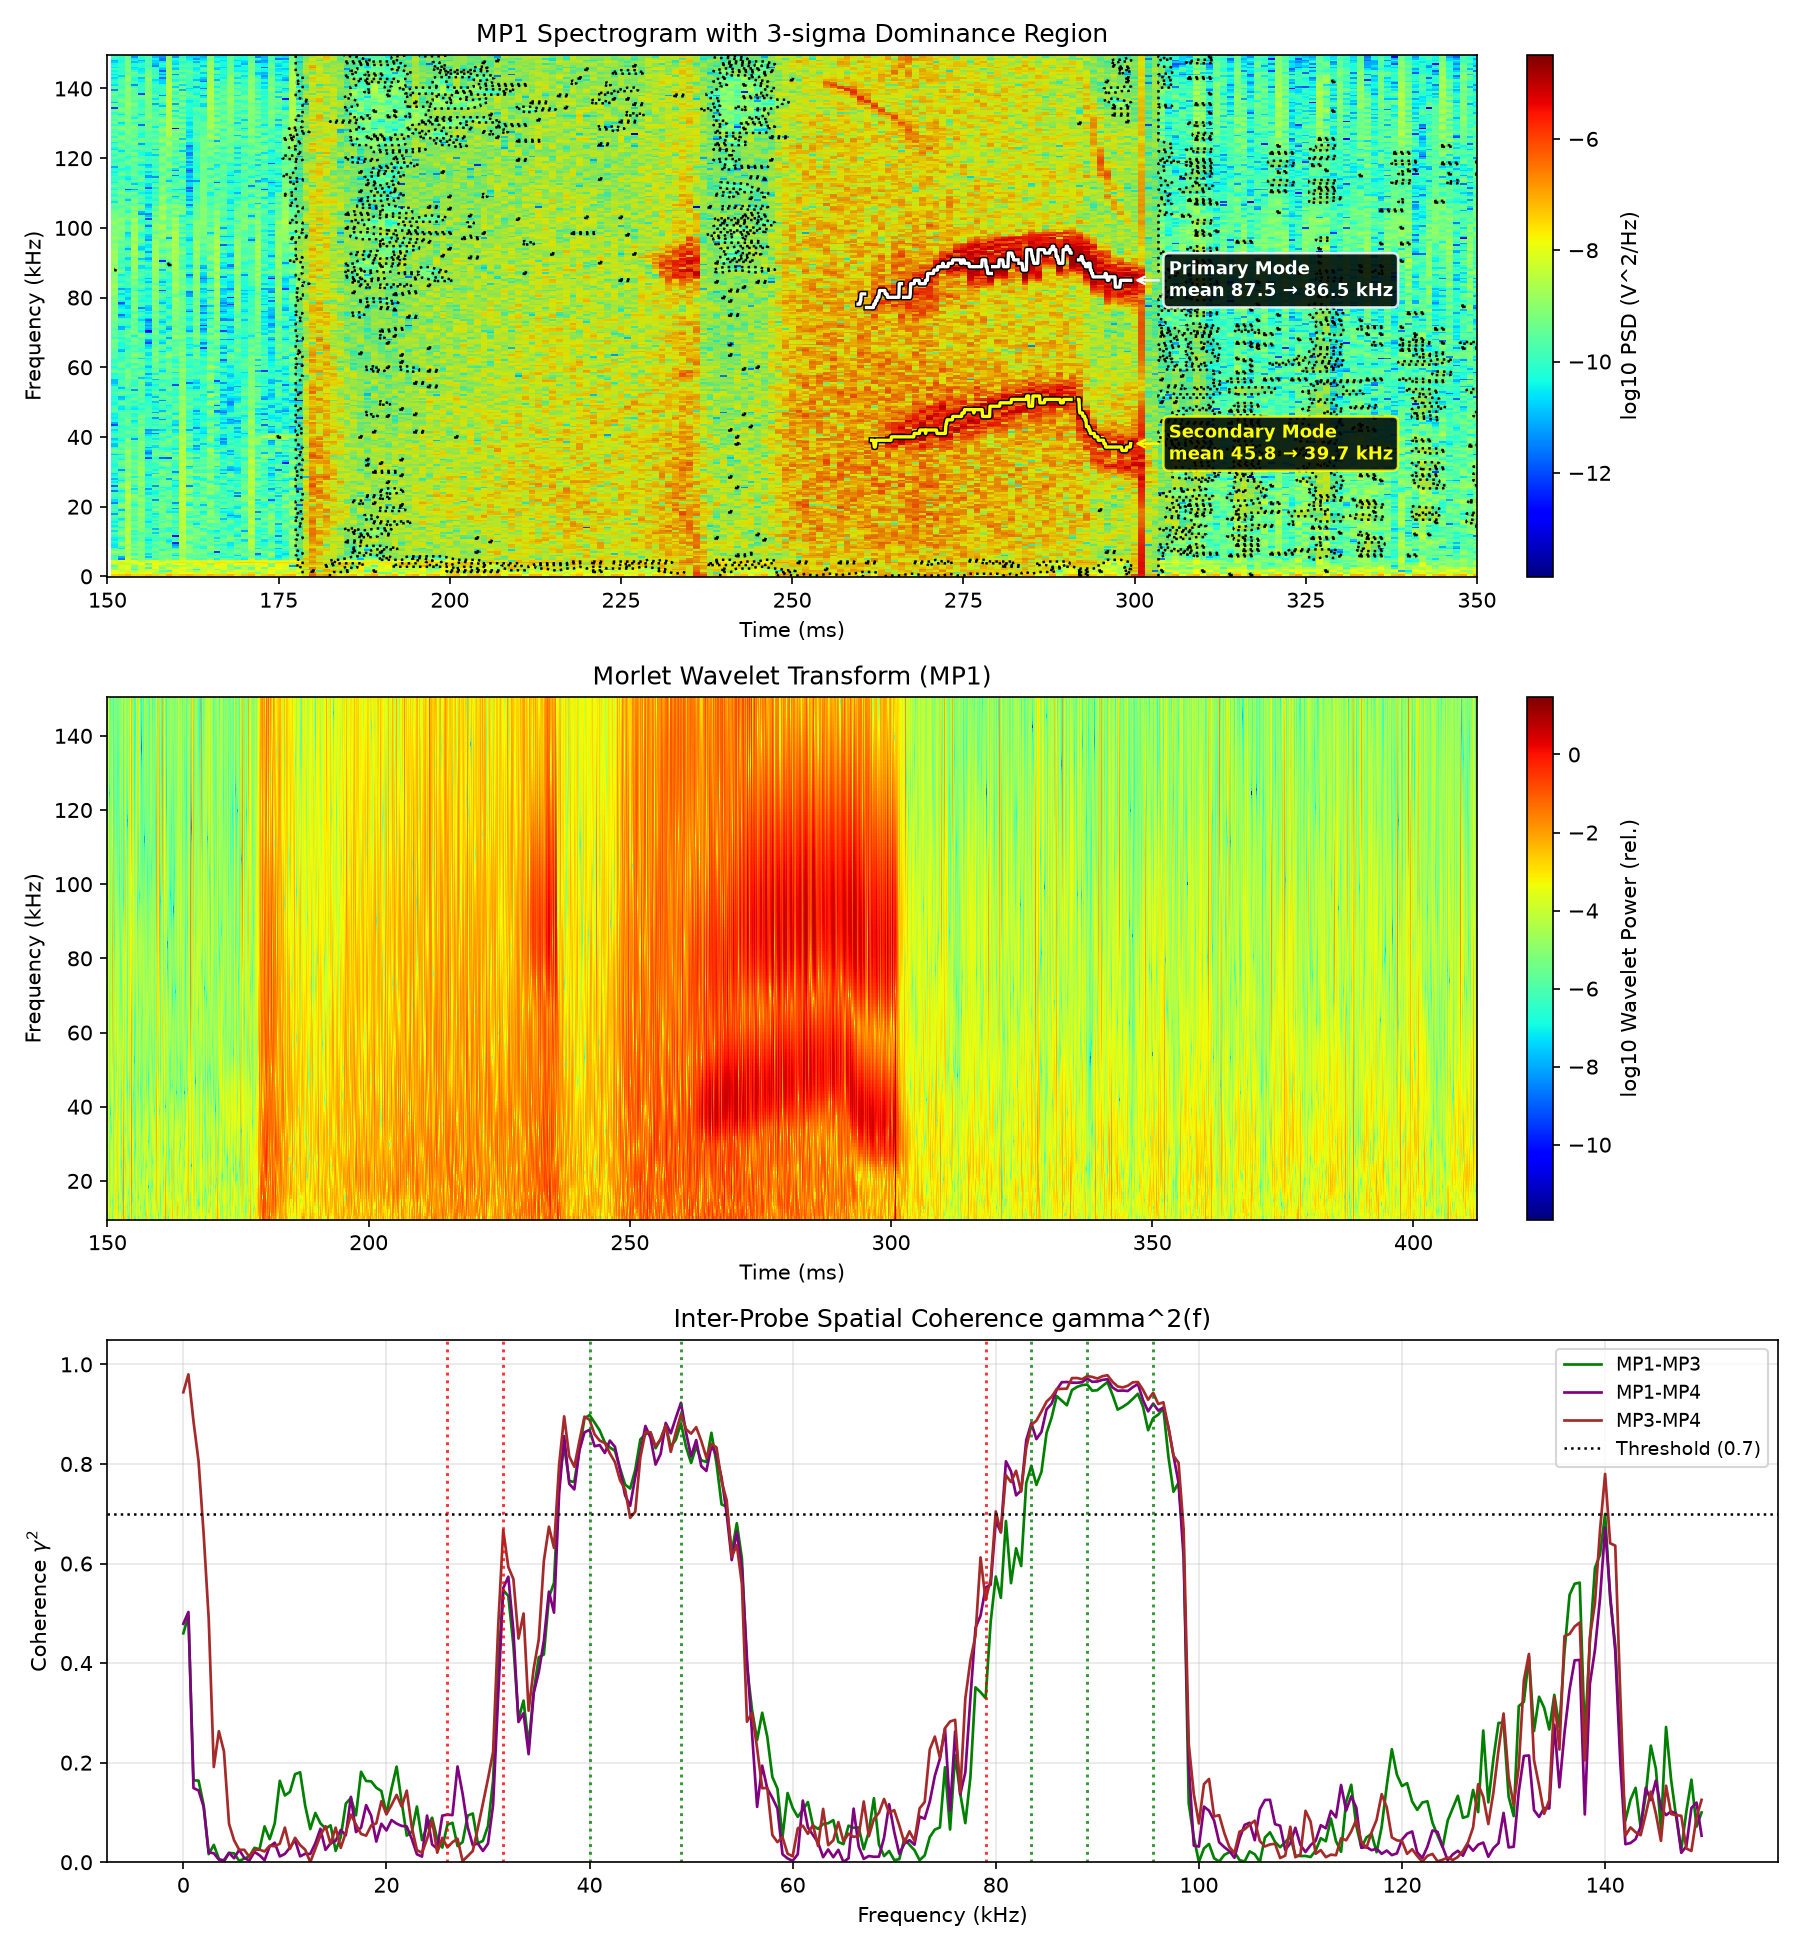
\includegraphics[height=0.85\textheight]{Images/obj1_mode_identification/mhd_analysis_objective1_88653.png}
    \end{figure}
\end{frame}

\begin{frame}{Backup: Objective 1 -- A Single, Validated Primary Mode (Full Window)}
    \begin{columns}[c]
        \begin{column}{0.44\textwidth}
            \centering
            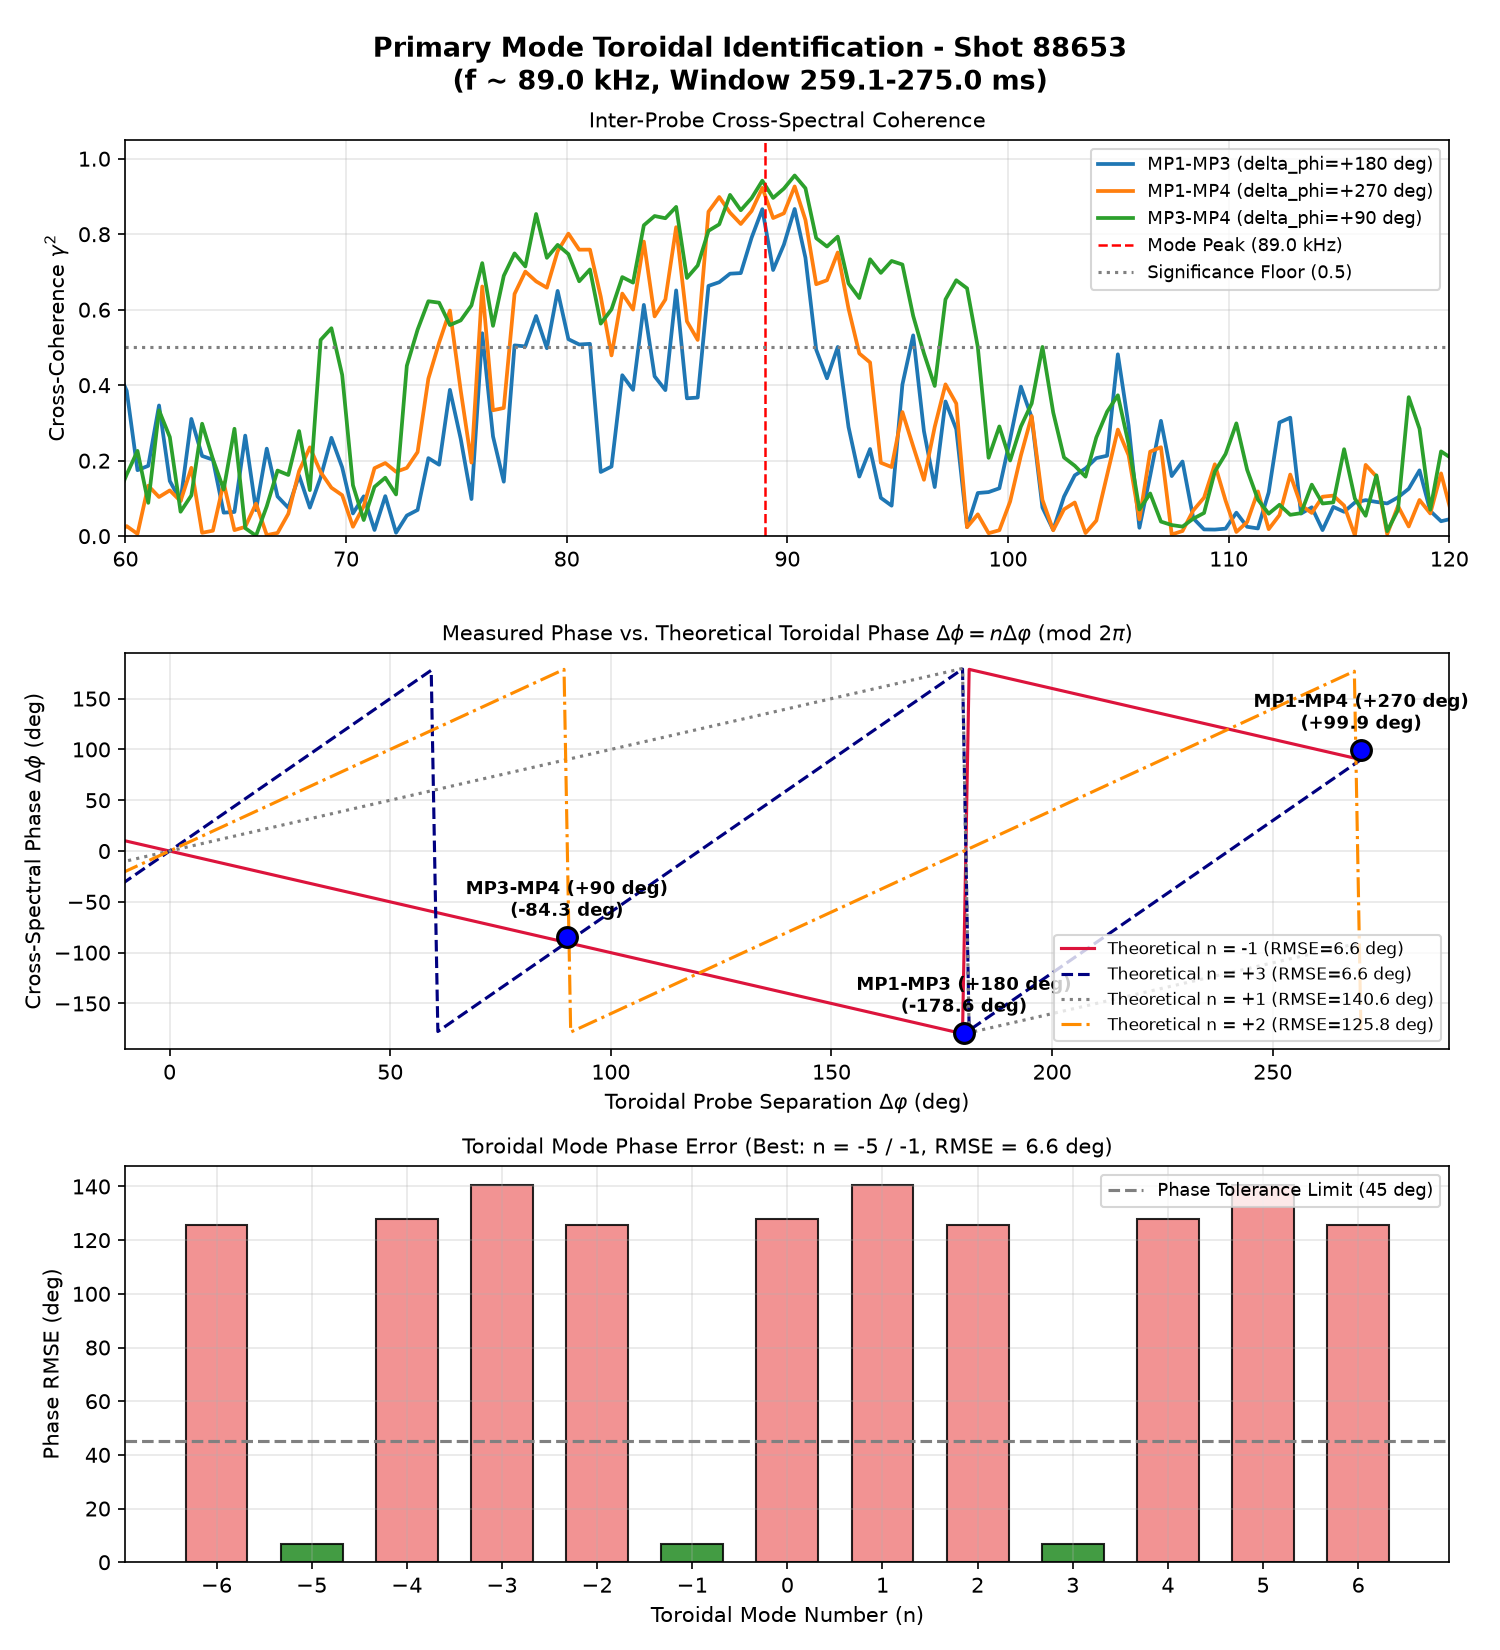
\includegraphics[height=0.84\textheight]{Images/obj1_mode_identification/mhd_primary_mode_toroidal_n_shot_88653.png}
        \end{column}
        \begin{column}{0.54\textwidth}
            \small
            \begin{itemize}
                \item \textbf{89.0 kHz} clears both criteria: $3\sigma$ dominance \emph{and}
                $\gamma^2=0.87$--$0.94$ across all Mirnov pairs (MP1-MP3: 0.87, MP1-MP4: 0.92,
                MP3-MP4: 0.94).
                \item Toroidal number $n\equiv-1$ (mod 4) is determined with three probes (RMSE $=\SI{6.6}{\degree}$).
                \item A nearby \SI{95.5}{kHz} peak is most likely the same chirping mode's
                spectral footprint, not a separate instability $\Rightarrow$ treated as
                \textbf{one} primary mode going forward.
            \end{itemize}
        \end{column}
    \end{columns}
\end{frame}

\begin{frame}{Backup: Objective 1 -- Spatial Structure \& Radial Localization}
    \centering
    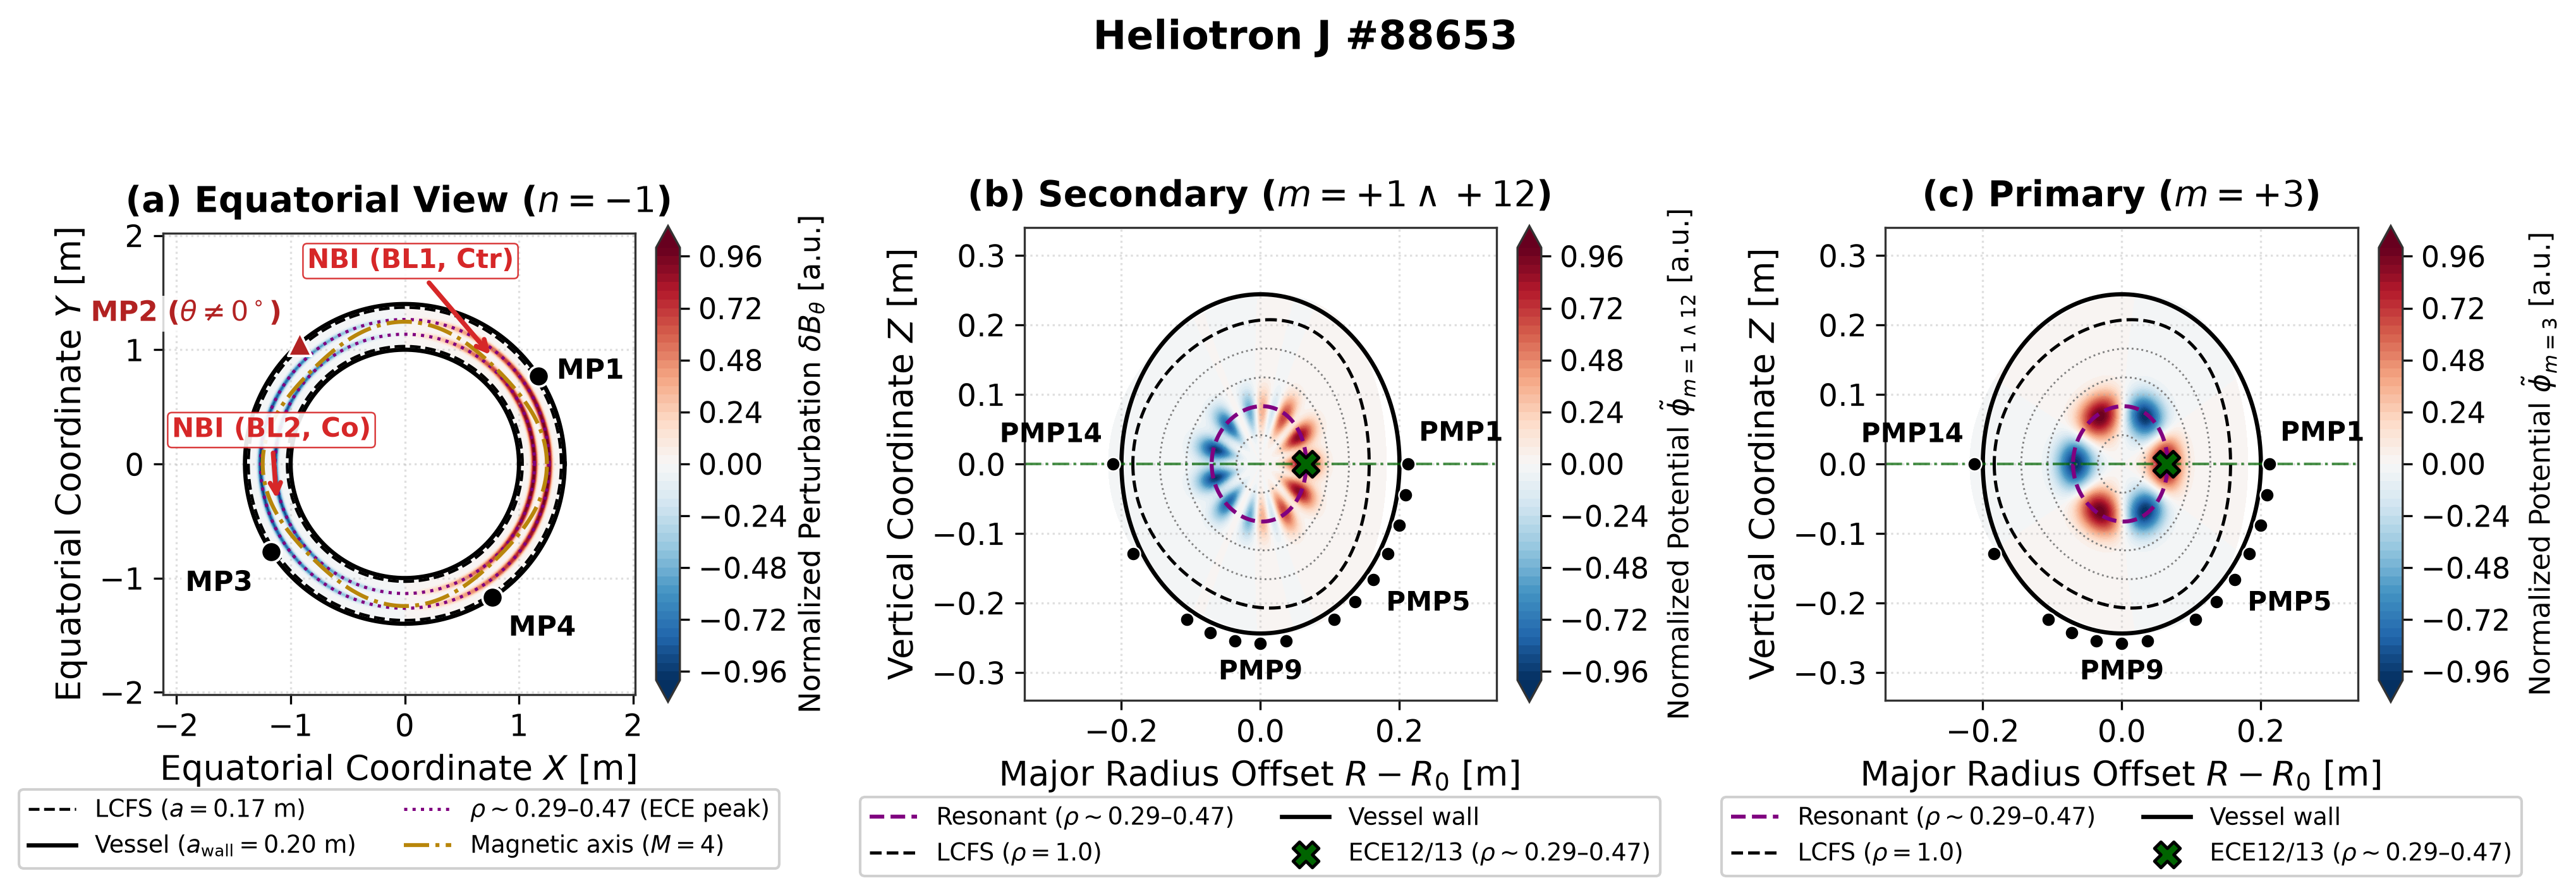
\includegraphics[width=0.62\textwidth]{Images/obj2_dynamics_and_structure/mhd_mode_spatial_map_2d_88653.png}
    \vspace{-0.1cm}
    \footnotesize
    \begin{itemize}
        \item Poloidal number $m=+3$: a single, coherent structure (top-down and poloidal cross-section agree).
        \item ECE fluctuation (\SIrange{80}{100}{kHz}) is largest at ECE12/13FAST
        (\SI{64.5}{GHz}/\SI{66.5}{GHz}; \SI{0.33}{V}/\SI{0.478}{V}, $\sim$200$\times$ the quiet level), near
        $\rho\approx0.62$. ECE12--13 are mutually coherent ($\gamma^2=0.77$) but not with MP1
        ($\gamma^2\approx0.06$ vs.\ floor 0.20): localization is suggestive only.
        \item Weak edge coupling at HAFAST7.5 ($\gamma^2=0.23$: above floor, below 0.7 gate).
    \end{itemize}
\end{frame}

\begin{frame}{Backup: Objective 1 -- Radial Fluctuation Profile}
    \begin{figure}[h!]
        \centering
        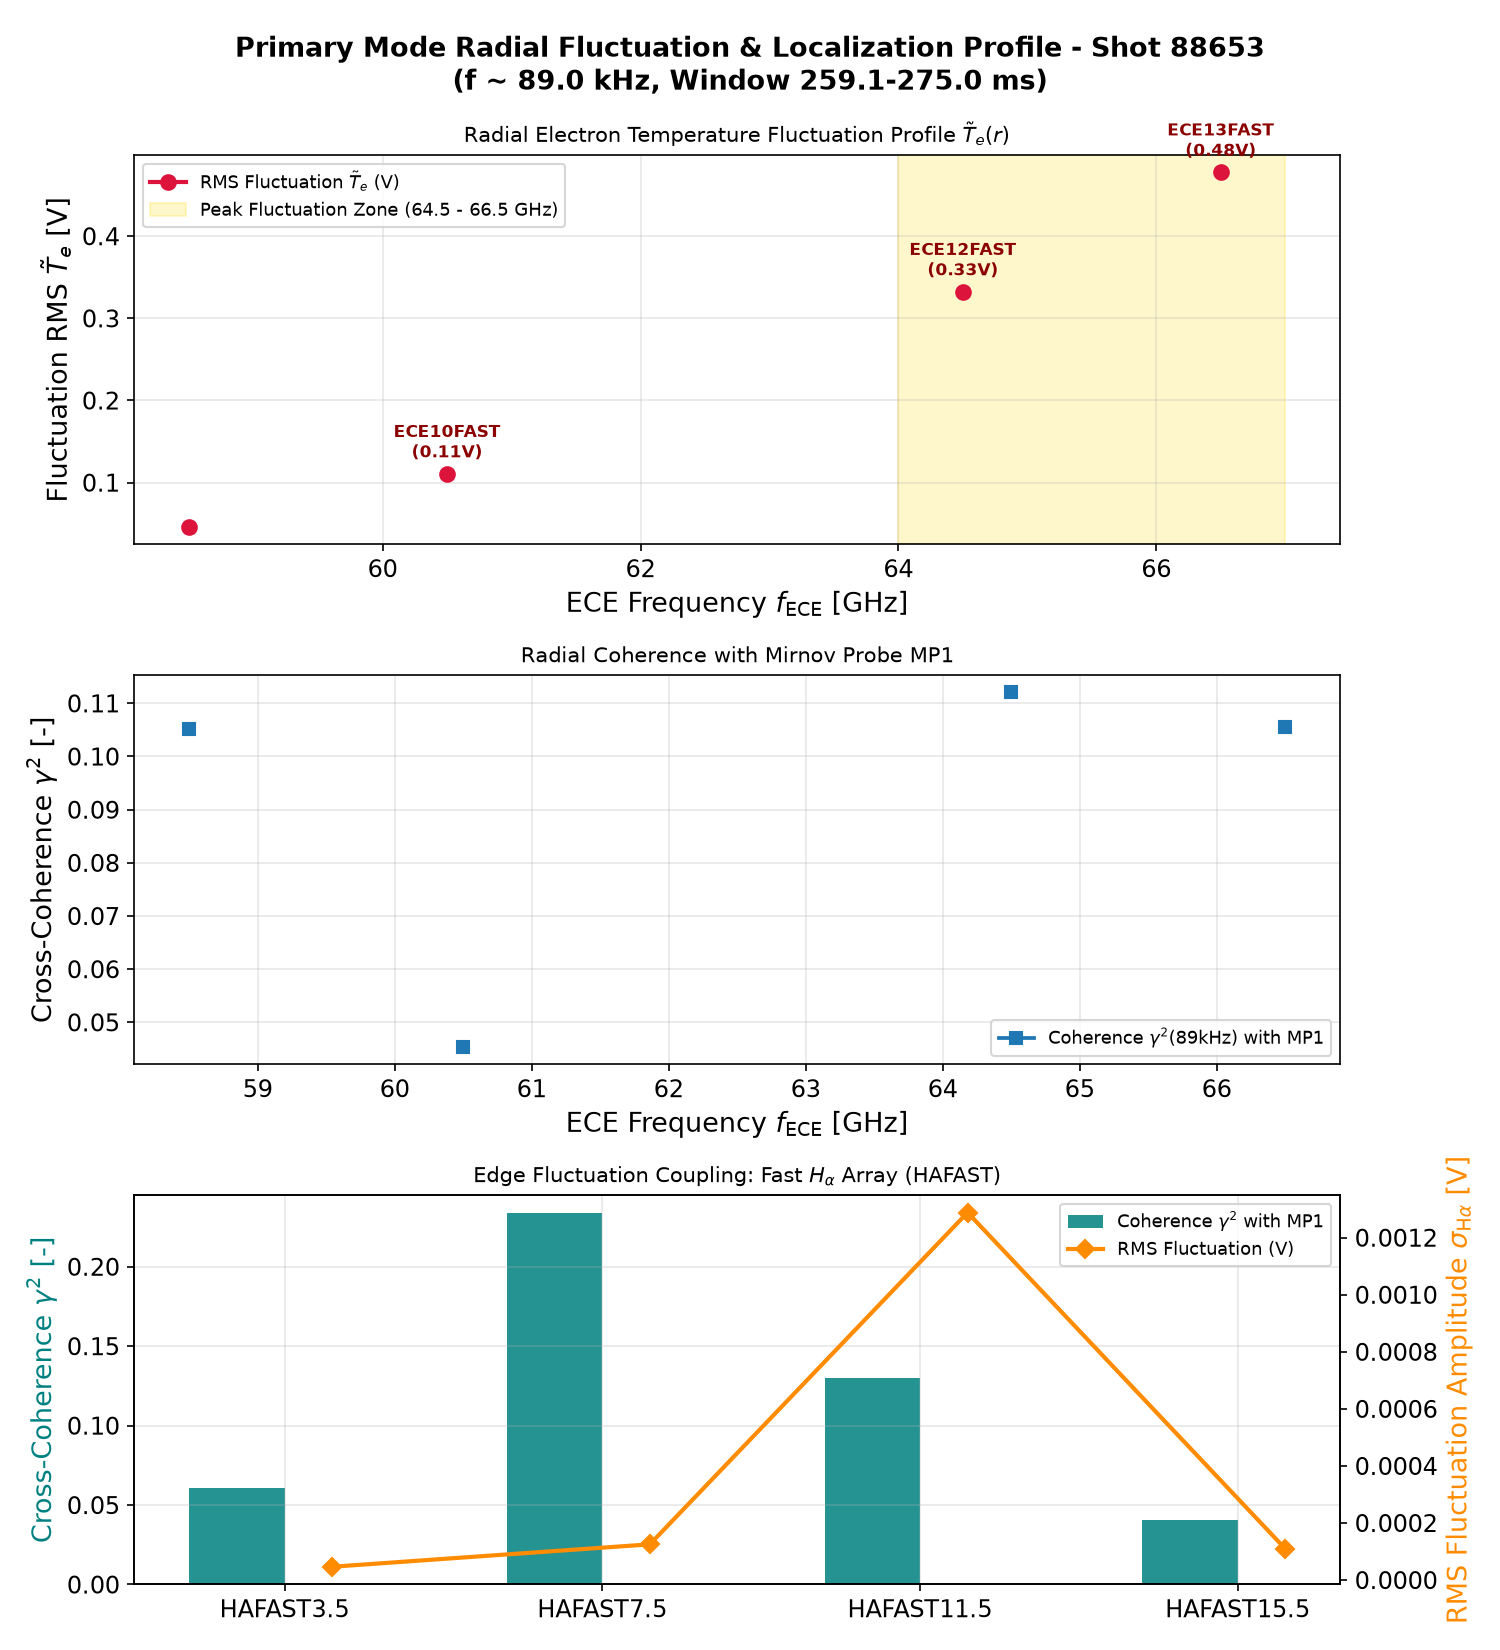
\includegraphics[height=0.74\textheight]{Images/obj1_mode_identification/mhd_primary_mode_radial_profile_shot_88653.png}
    \end{figure}
    \vspace{-0.3cm}
    {\tiny RMS of the \SIrange{80}{100}{kHz} band, \SIrange{259.1}{275.0}{ms}. Omitted: ECE1--7, 11, 14 (active = quiet RMS: dead or outside the plasma) and ECE8, 15, 16 ($<0.01$\,V). ECE12--13 are mutually coherent (0.77 at \SI{89}{kHz}); ECE--MP1 coherence (0.05--0.11) is below its floor (0.20).}
\end{frame}

\begin{frame}{Backup: Objective 1 -- Mode Identity Survives ECH Shut-off}
    \small
    \centering
    \begin{tabular}{lccccc}
        \toprule
        Window & $f$ (kHz) & $n$ (aliased) & RMSE ($^\circ$) & $\gamma^2$ range \\
        \midrule
        ECH+NBI  & 89.0 & $-5$ ($\equiv -1$) & 5.2 & 0.96--0.98 \\
        NBI-only & 86.0 & $-5$ ($\equiv -1$) & 6.7 & 0.997--0.998 \\
        \bottomrule
    \end{tabular}
    \vspace{0.3cm}
    \normalsize
    \begin{itemize}
        \item The \textbf{same toroidal number and helicity} persist after ECH
        shuts off; only the frequency downshifts ($\sim$2--\SI{3}{kHz} primary: PSD peak
        89.0$\to$87.0, $n$-fit line 89.0$\to$86.0; $\sim$\SI{11.5}{kHz} secondary) -- consistent with electron
        cooling (lower sound speed) or a rotation/Doppler shift.
        \item In both windows $3\sigma$ occupancy is 100\%: the mode is
        \textbf{continuously sustained} by the NBI fast-ion drive, not decaying --
        but it hops discretely among 2--3 frequency branches
        ($\sim$0.4--1.3 jumps/ms), a hallmark of EPM/BAE avalanche (hole-clump)
        dynamics.
        \item \textbf{Reproduces in an independent shot:} validation shot
        \#88654 shows the same mode structure -- same rank order,
        comparable amplitudes, comparable or higher coherence -- downshifted
        $\sim$1--\SI{2.5}{kHz} (backup).
    \end{itemize}
\end{frame}

\begin{frame}{Backup: Objective 1 Comparative -- Mode Identification Overview}
    \begin{columns}[T]
        \begin{column}{0.4\textwidth}
            \centering ECH+NBI\\
            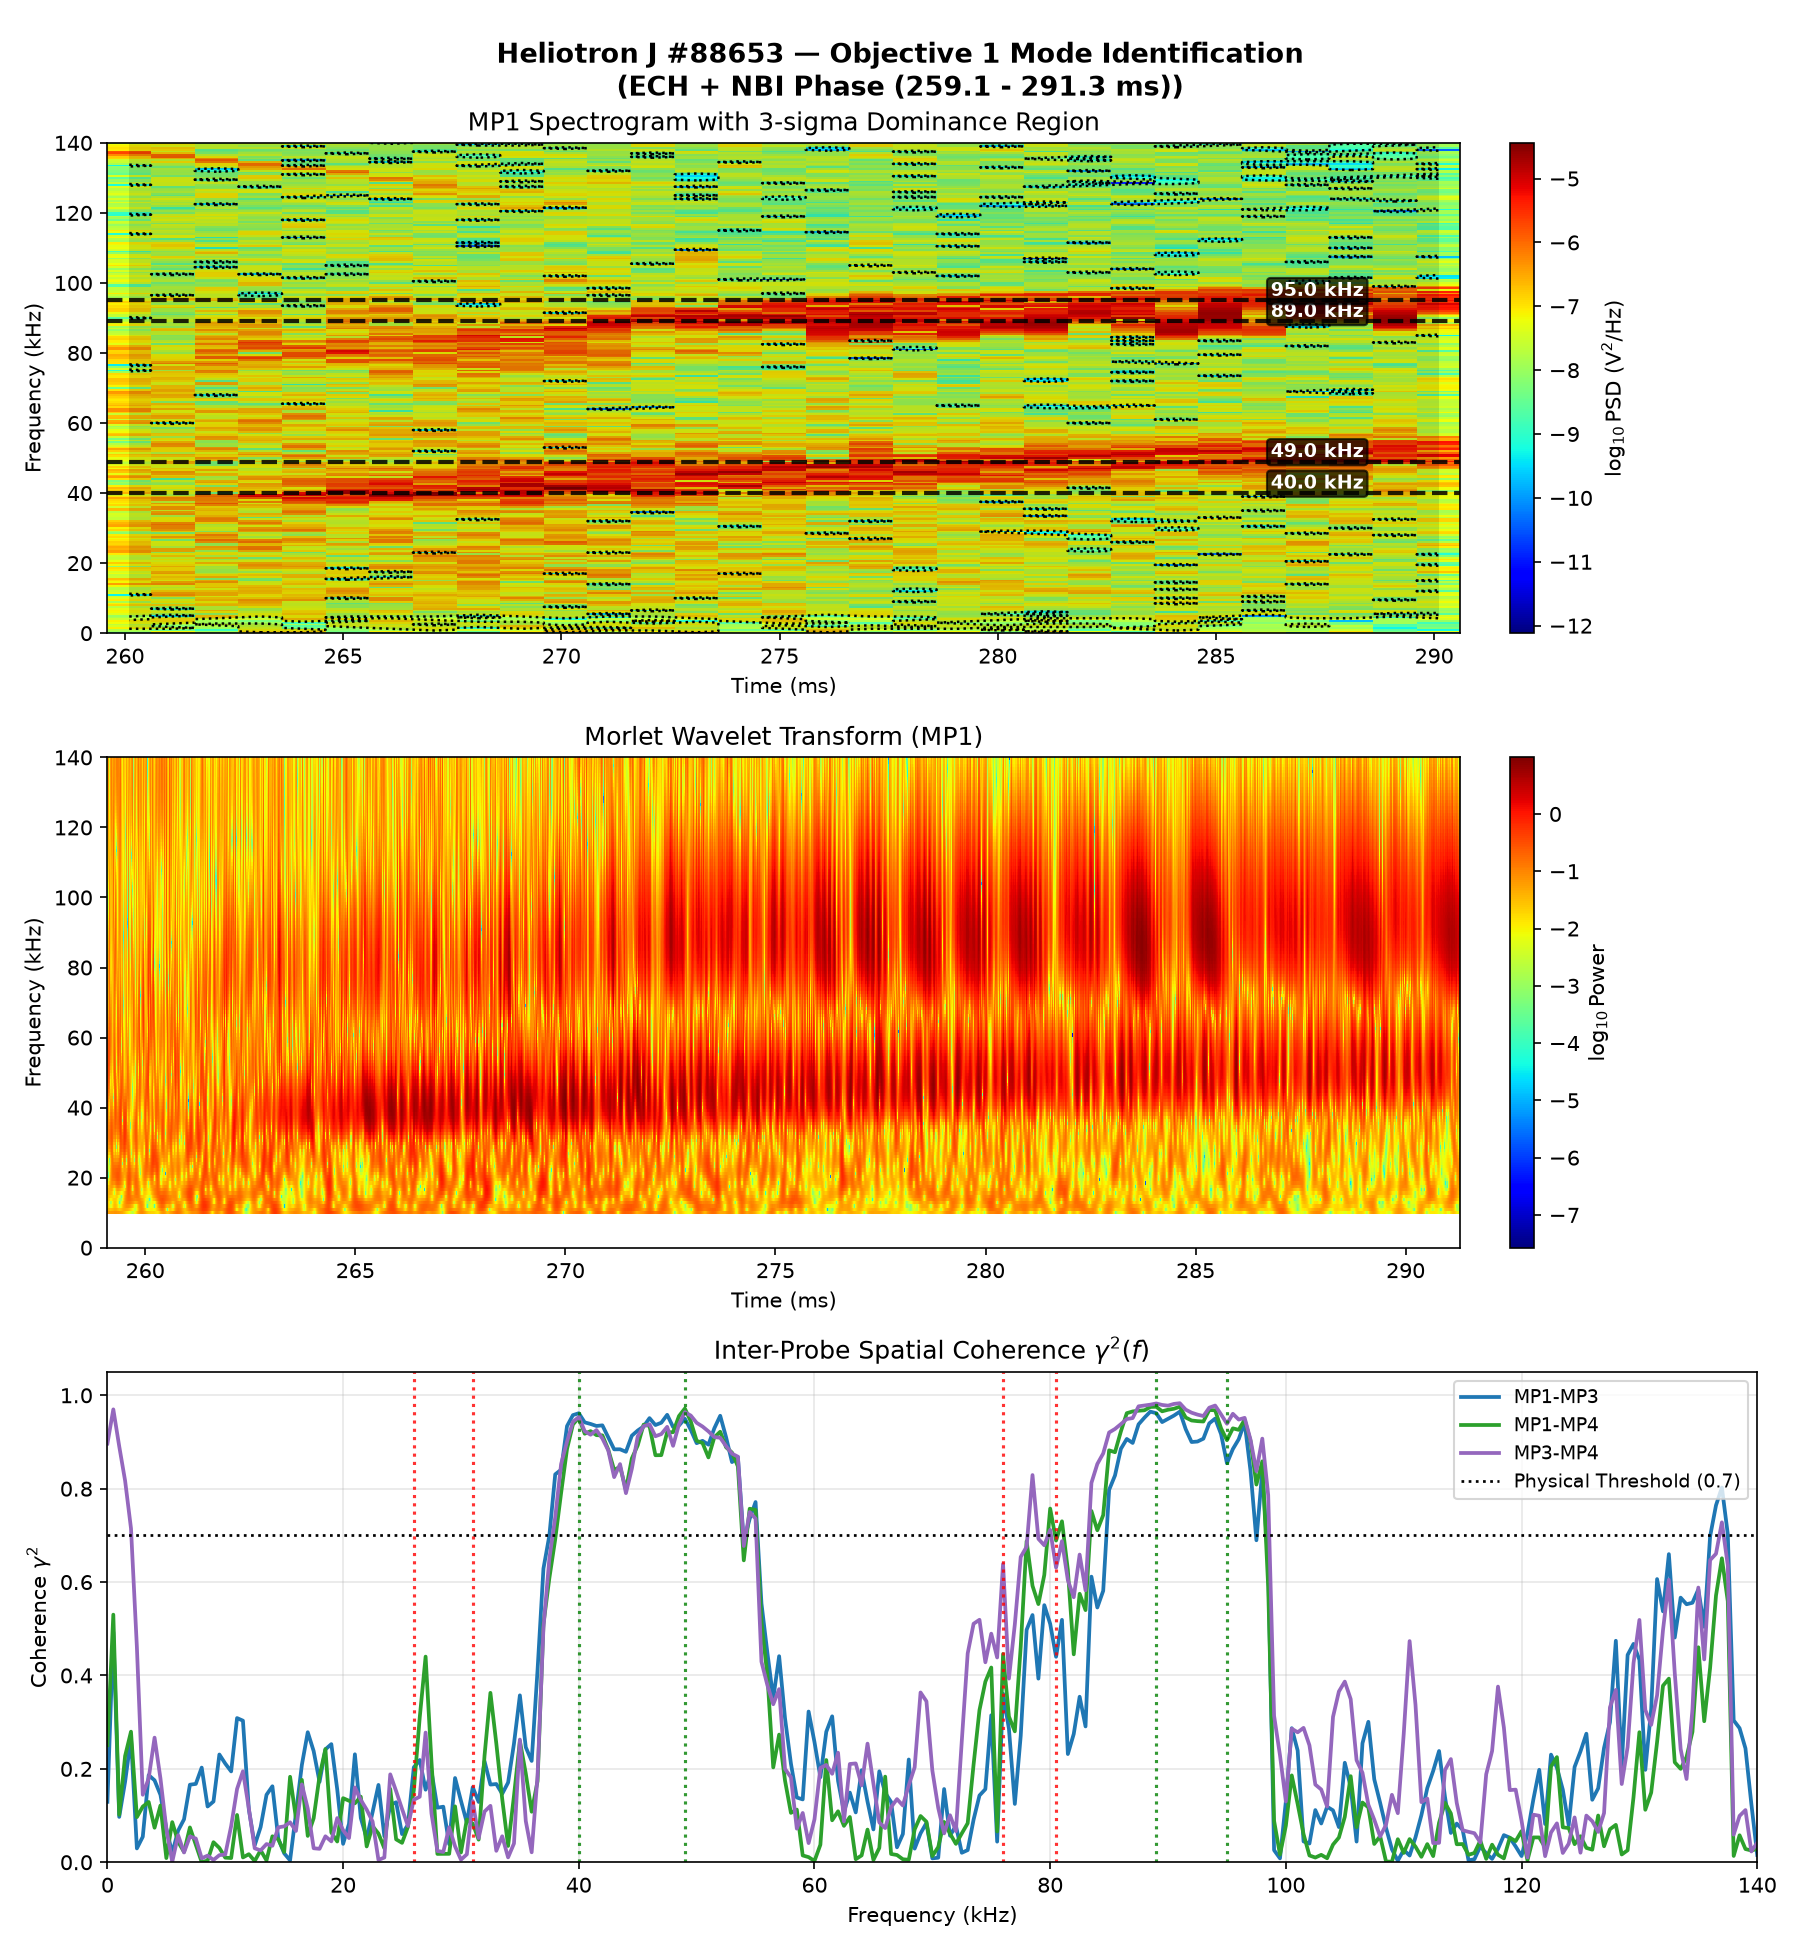
\includegraphics[width=\textwidth]{Images/heating_phase_comparison/mhd_analysis_objective1_88653_ECH_NBI.png}
        \end{column}
        \begin{column}{0.4\textwidth}
            \centering NBI-only\\
            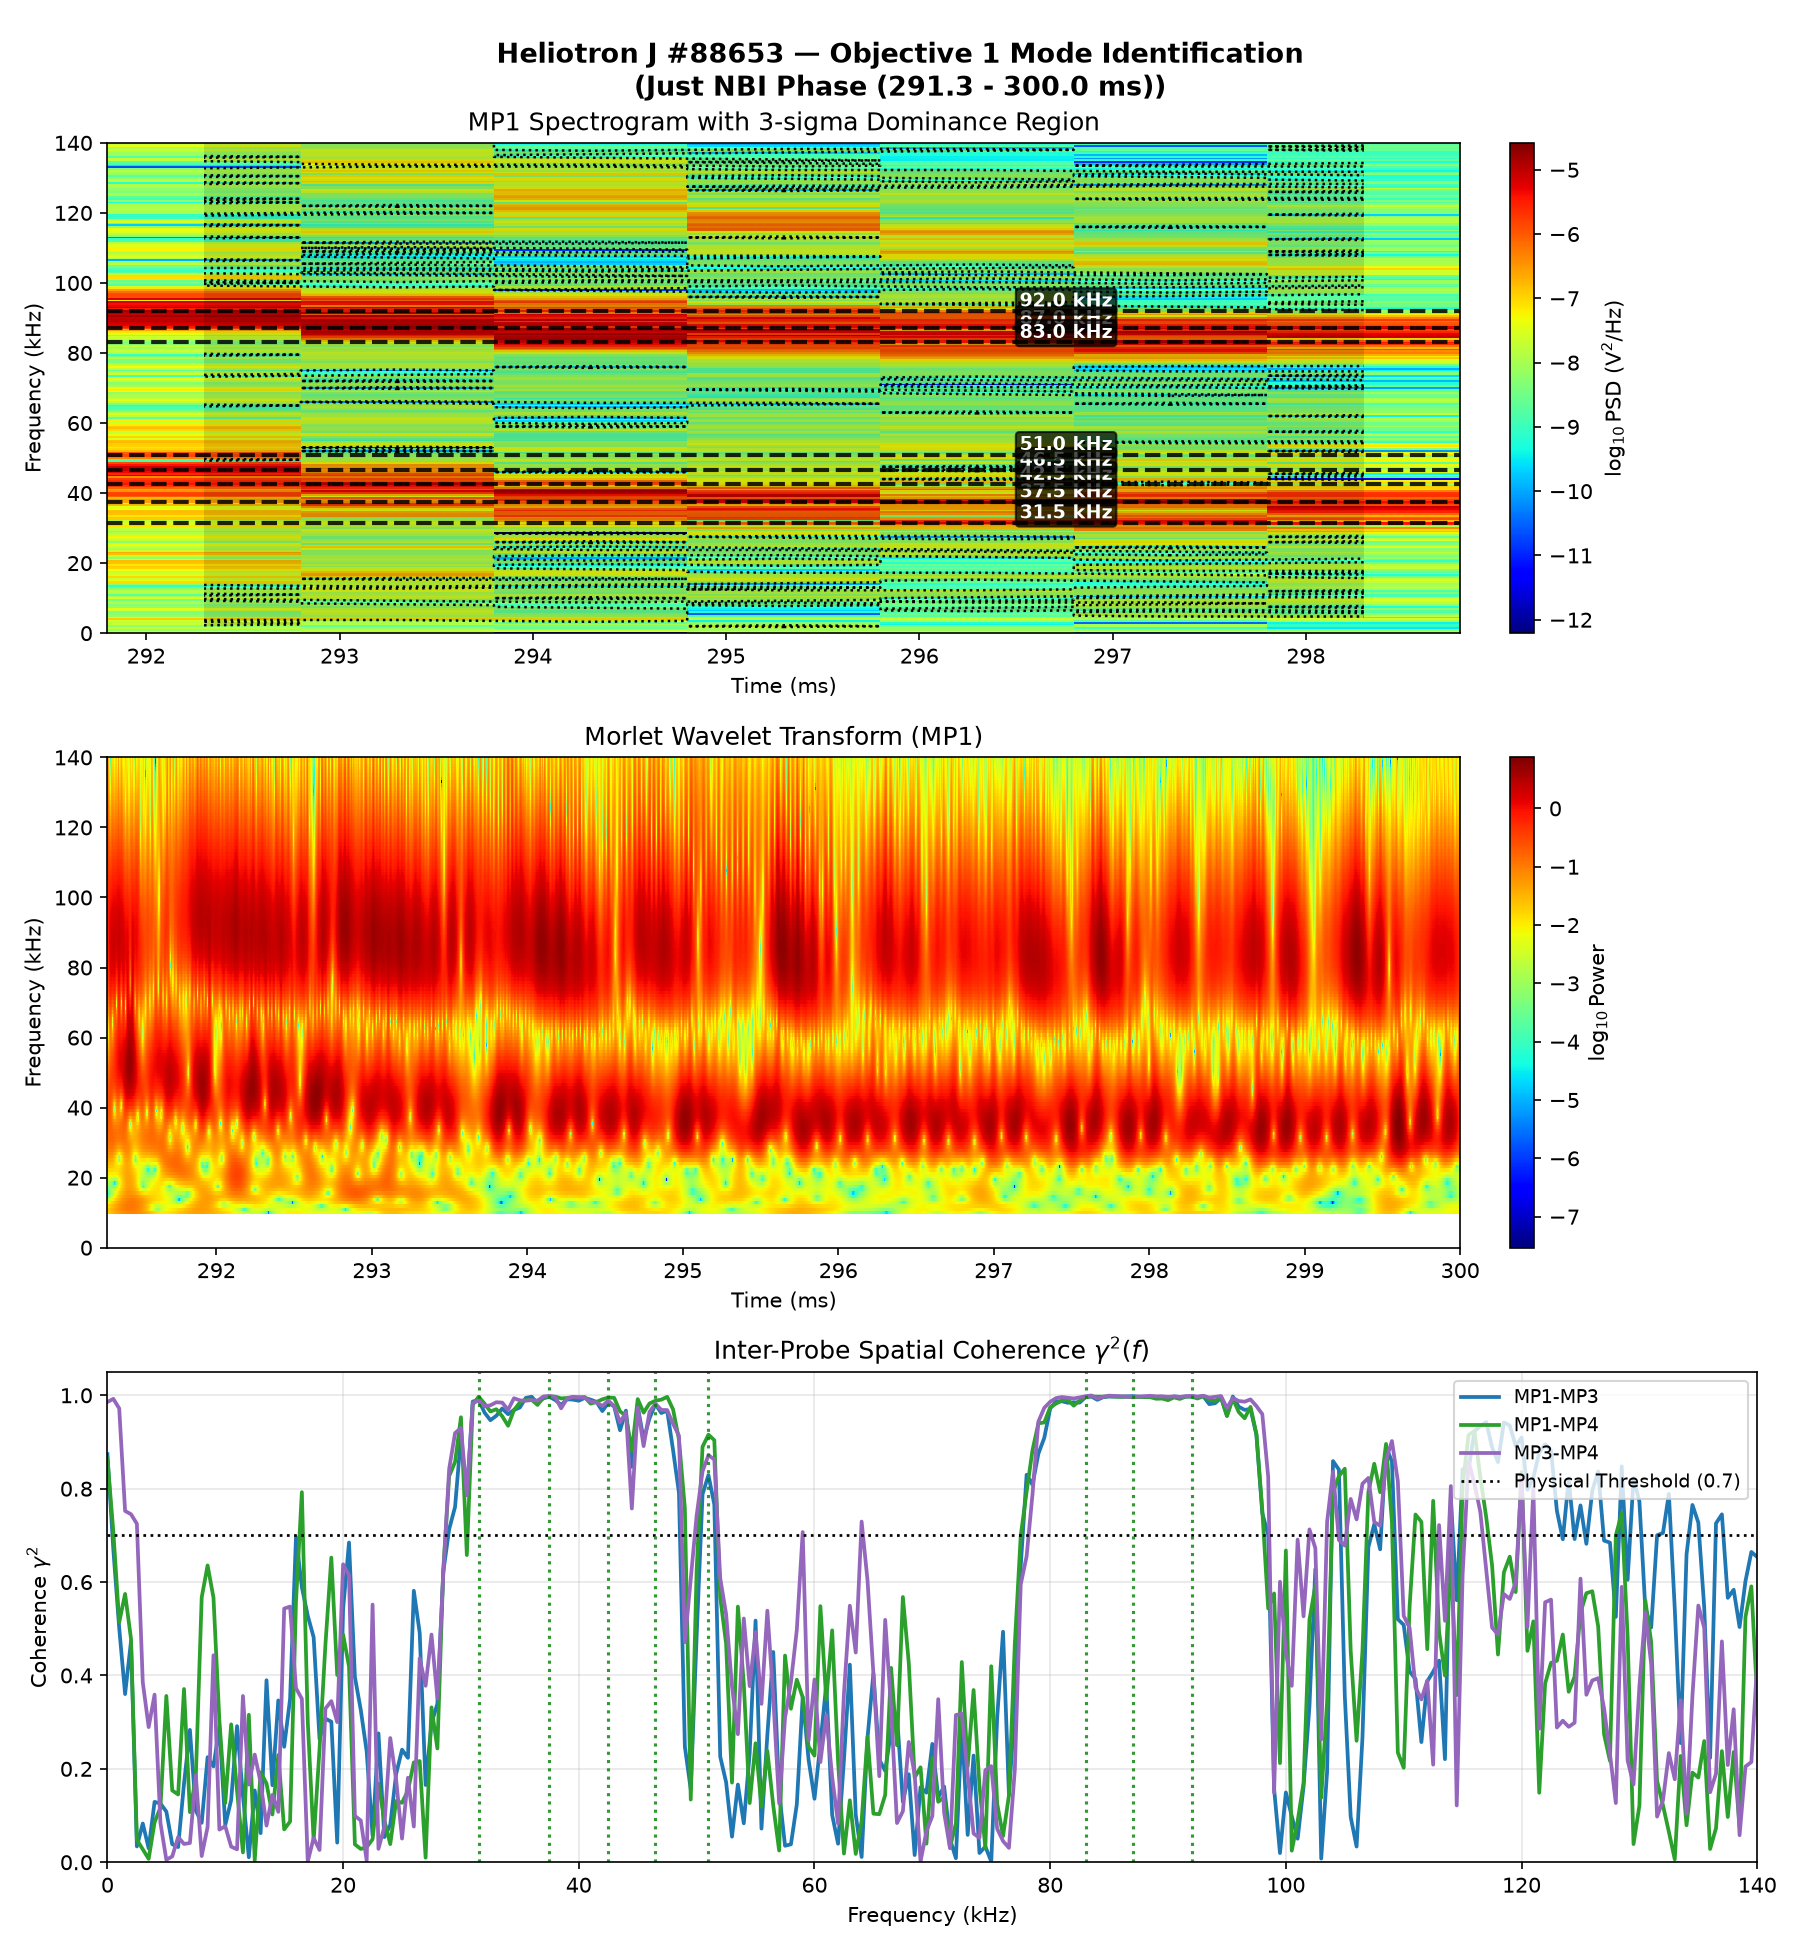
\includegraphics[width=\textwidth]{Images/heating_phase_comparison/mhd_analysis_objective1_88653_NBI_only.png}
        \end{column}
    \end{columns}
\end{frame}

\begin{frame}{Backup: Objective 1 Comparative -- Confirmed Discrete Modes}
    \tiny
    \setlength{\tabcolsep}{5pt}
    \begin{columns}[T]
        \begin{column}{0.48\textwidth}
            \centering \normalsize\textbf{ECH+NBI}\tiny
            \begin{tabular}{cc@{\hspace{6pt}}ccc}
                \toprule
                $f$ (kHz) & Amp. (a.u.) & $\gamma^2_{13}$ & $\gamma^2_{14}$ & $\gamma^2_{34}$ \\
                \midrule
                89.0 & \num{5.36e-6} & 0.962 & 0.975 & 0.983 \\
                49.0 & \num{3.05e-6} & 0.950 & 0.972 & 0.964 \\
                40.0 & \num{2.89e-6} & 0.962 & 0.952 & 0.953 \\
                95.0 & \num{1.78e-6} & 0.854 & 0.904 & 0.939 \\
                \bottomrule
            \end{tabular}
            \vspace{0.15cm}
            \raggedright 4 additional candidates (80.5, 26.0, 76.0, 31.0 kHz) were above the noise floor but failed the coherence criterion.
        \end{column}
        \begin{column}{0.48\textwidth}
            \centering \normalsize\textbf{NBI-only}\tiny
            \begin{tabular}{cc@{\hspace{6pt}}ccc}
                \toprule
                $f$ (kHz) & Amp. (a.u.) & $\gamma^2_{13}$ & $\gamma^2_{14}$ & $\gamma^2_{34}$ \\
                \midrule
                37.5 & \num{8.24e-6} & 0.997 & 0.997 & 0.999 \\
                87.0 & \num{6.76e-6} & 0.998 & 0.996 & 0.997 \\
                83.0 & \num{3.90e-6} & 0.996 & 0.996 & 0.998 \\
                92.0 & \num{3.43e-6} & 0.998 & 0.997 & 0.999 \\
                42.5 & \num{2.41e-6} & 0.984 & 0.995 & 0.989 \\
                31.5 & \num{1.85e-6} & 0.990 & 0.997 & 0.989 \\
                46.5 & \num{1.21e-6} & 0.981 & 0.988 & 0.982 \\
                51.0 & \num{2.17e-7} & 0.829 & 0.916 & 0.872 \\
                \bottomrule
            \end{tabular}
        \end{column}
    \end{columns}
    \vspace{0.2cm}
    \normalsize
    \textbf{Observation:} every candidate mode passes the dual criterion once ECH switches off, and coherence pairs are systematically higher -- consistent with a cleaner, more coherent fluctuation spectrum in the NBI-only phase.
\end{frame}

\subsection{Backup: Objective 2}

\begin{frame}{Backup: Objective 2 -- Two Bands, Poloidal Structure and Scaling Tests}
    \begin{columns}[c]
        \begin{column}{0.36\textwidth}
            \centering
            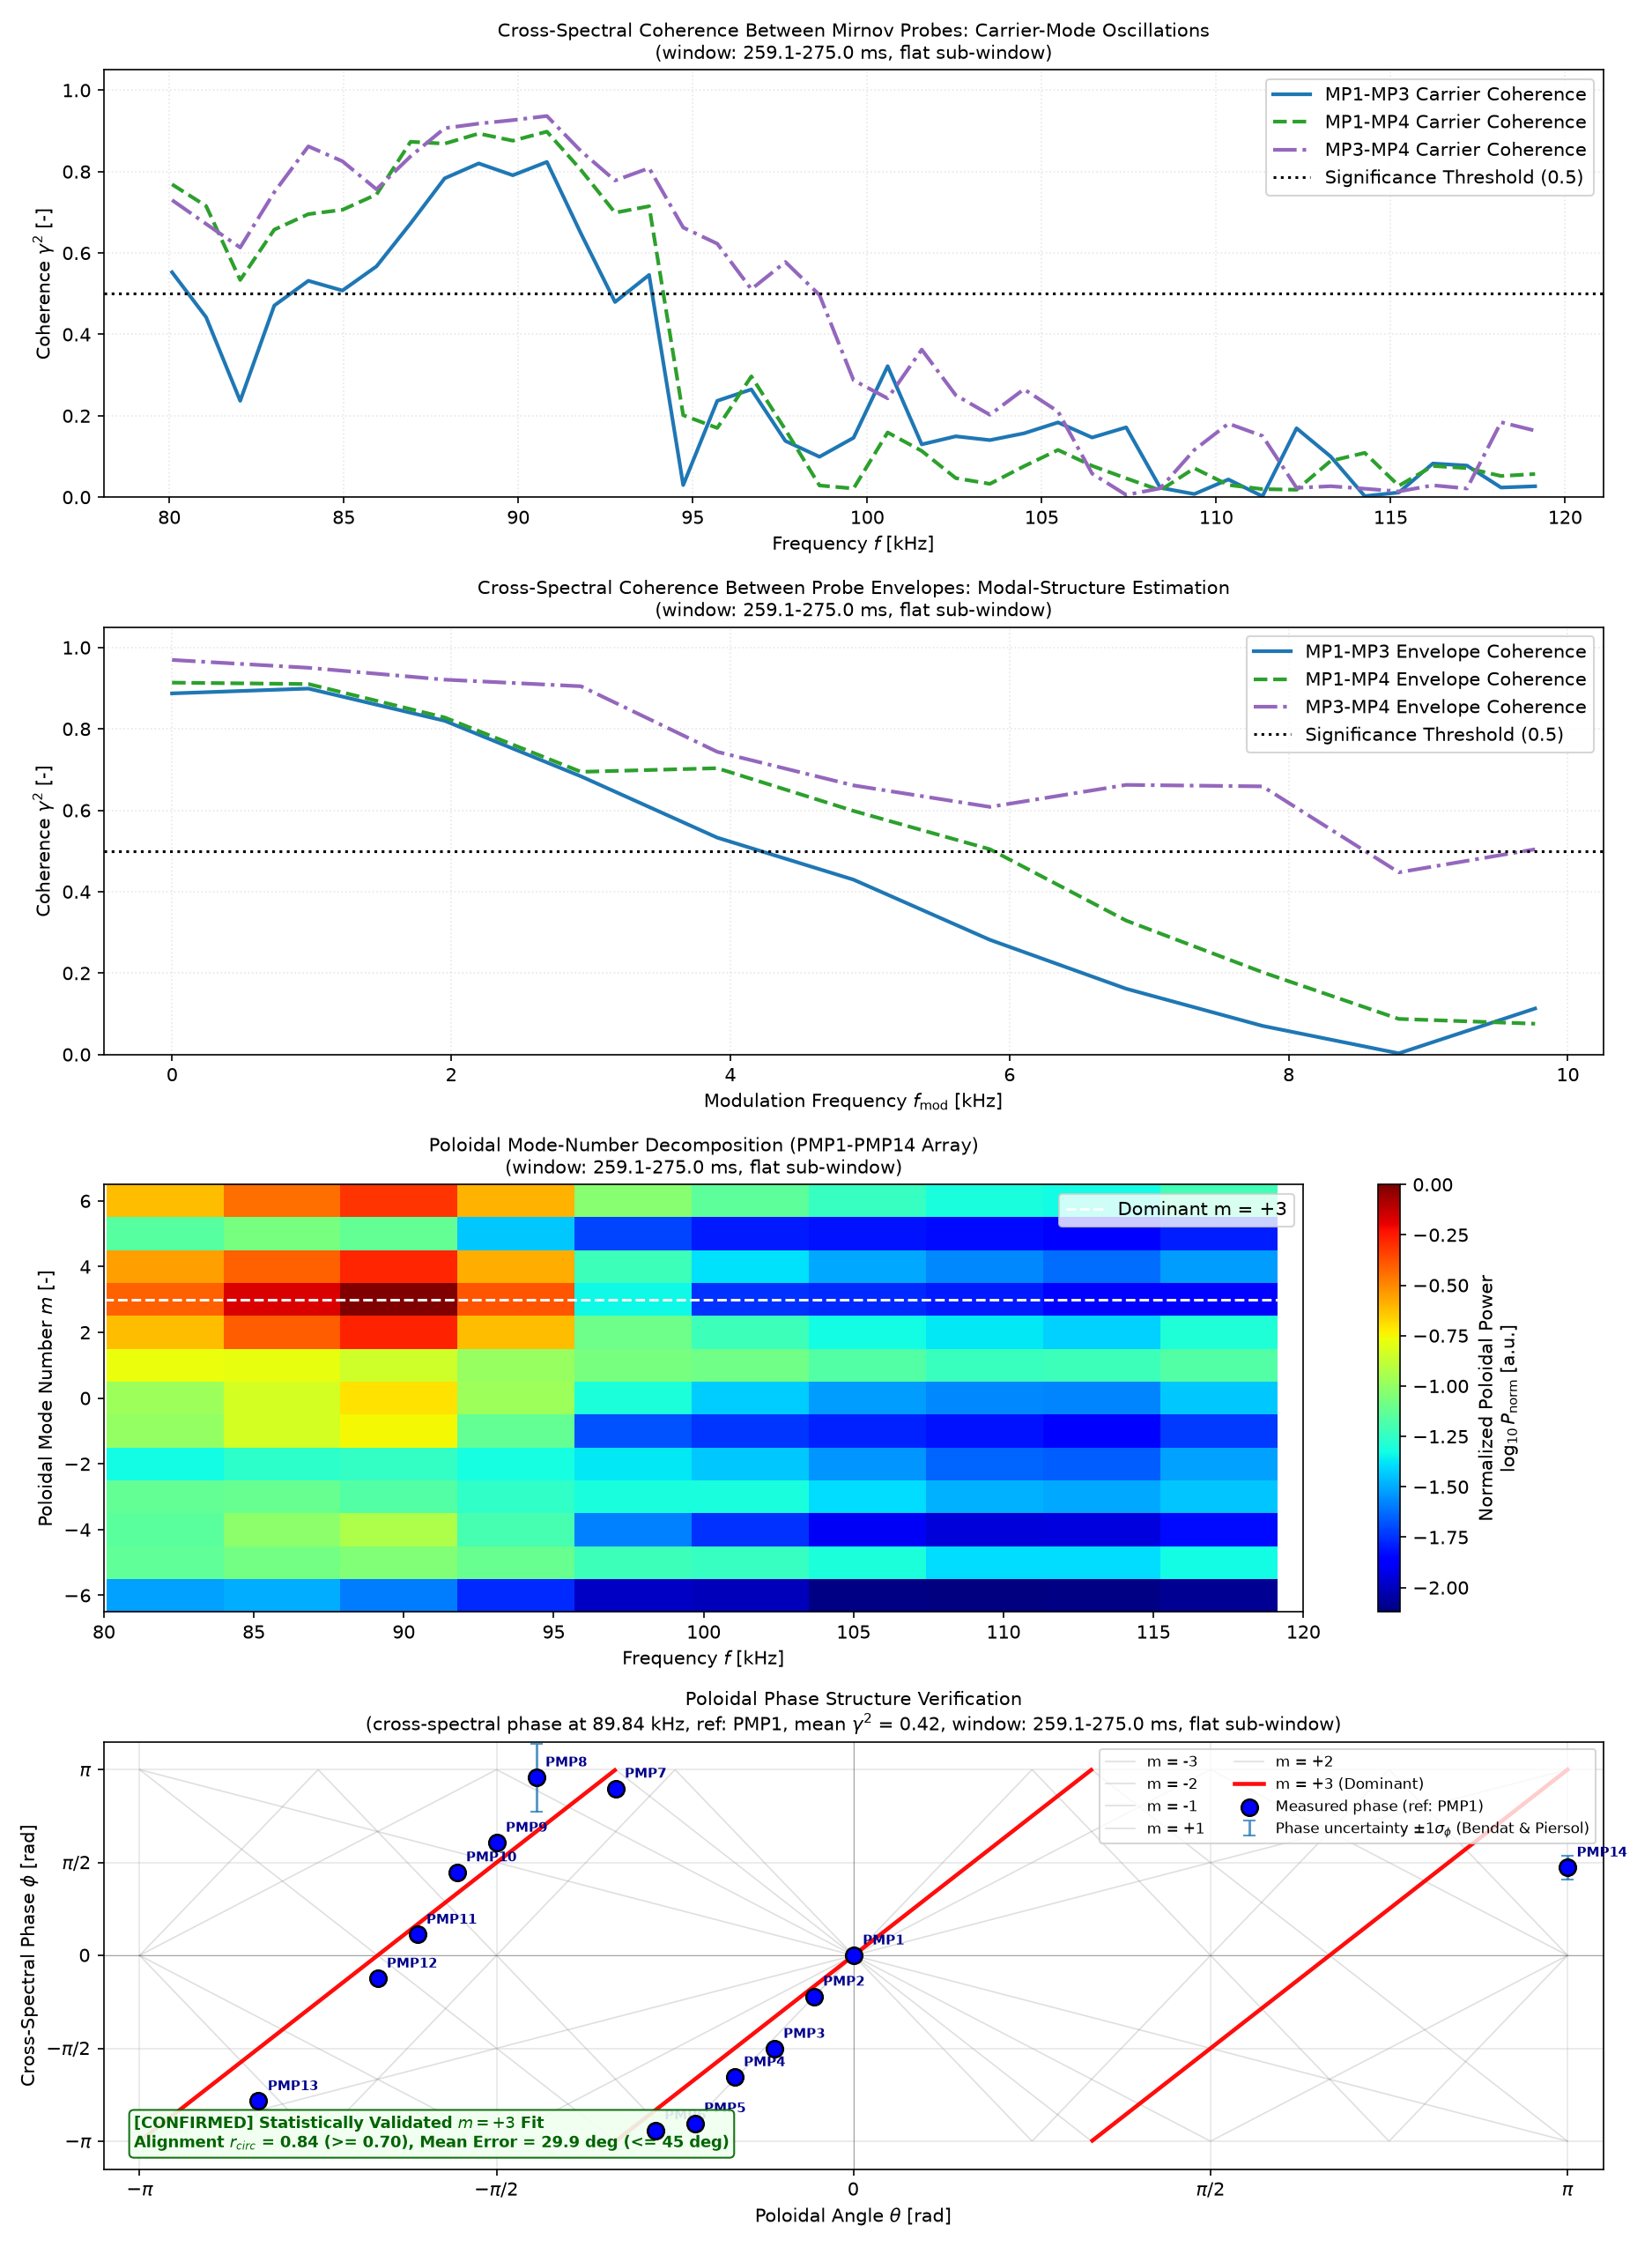
\includegraphics[height=0.84\textheight]{Images/obj2_dynamics_and_structure/mhd_analysis_objective2_structure_88653_80_120kHz.png}
        \end{column}
        \begin{column}{0.62\textwidth}
            \small
            \begin{itemize}
                \item \textbf{Primary (\SIrange{80}{120}{kHz}):} $m=+3$ \textbf{confirmed} in both windows
                ($r_{\text{circ}}$ up to 0.90), $f=\SI{89.84}{kHz}$; highest-$|r|$ scaling model
                BAE/GAM ($\sqrt{T_e}$): $r=-0.48$ ($p=0.20$).
                \item \textbf{Secondary (\SIrange{40}{80}{kHz}):} $m$ tentative ($+6\to+2$ between
                windows; $r_{\text{circ}}<0.7$), $f=\SI{42.97}{kHz}$; highest-$|r|$ model
                current-induced ($I_p$): $r=-0.85$ ($p=0.16$).
                \item \textbf{Scaling tests:} none of six models is significant
                (adjusted $p>0.16$; $N_{\text{eff}}\approx4$ for Secondary, $\approx9$ for Primary), and both
                top-$|r|$ models have the sign opposite to their prediction -- no model is identified.
            \end{itemize}
        \end{column}
    \end{columns}
\end{frame}

\begin{frame}{Backup: Objective 2 -- EPM--Heating Statistical Correlation Metrics}
    \small
    \begin{center}
    \begin{tabular}{lcc}
        \toprule
        Correlation with mode envelope & Secondary band ($r$) & Primary band ($r$) \\
        \midrule
        Plasma current $I_p$        & 0.801 & 0.758 \\
        Stored energy $W_p$         & 0.810 & 0.784 \\
        Line-averaged density $n_e$ ($t\ge270$\,ms) & 0.874 & 0.867 \\
        Fast H$\alpha$ emission     & 0.609 & 0.568 \\
        \midrule
        NBI power (direct)          & $\sim$0.61--0.64 & $\sim$0.61--0.64 \\
        ECH power (direct)          & $\sim$0.44--0.45 & $\sim$0.44--0.45 \\
        ECH power (\emph{partial}, step removed) & 0.06--0.12 & 0.06--0.12 \\
        \bottomrule
    \end{tabular}
    \end{center}
    \vspace{0.3cm}
    \normalsize
    Once the shared ECH-on/off step is partialled out, the ECH correlation nearly
    vanishes while the NBI correlation survives $\Rightarrow$ consistent with
    drive by the \textbf{NBI fast-ion population} rather than ECH. Caveat: NBI
    is also an on/off step shared with all plasma signals, and $I_p$, $W_p$,
    $n_e$ correlate more strongly (0.76--0.87); the series are strongly
    autocorrelated, so the correlations are descriptive, not tests.
\end{frame}

\begin{frame}{Backup: Objective 2 -- The Carrier Talks to Its Own Envelope}
    \begin{columns}[c]
        \begin{column}{0.58\textwidth}
            \centering
            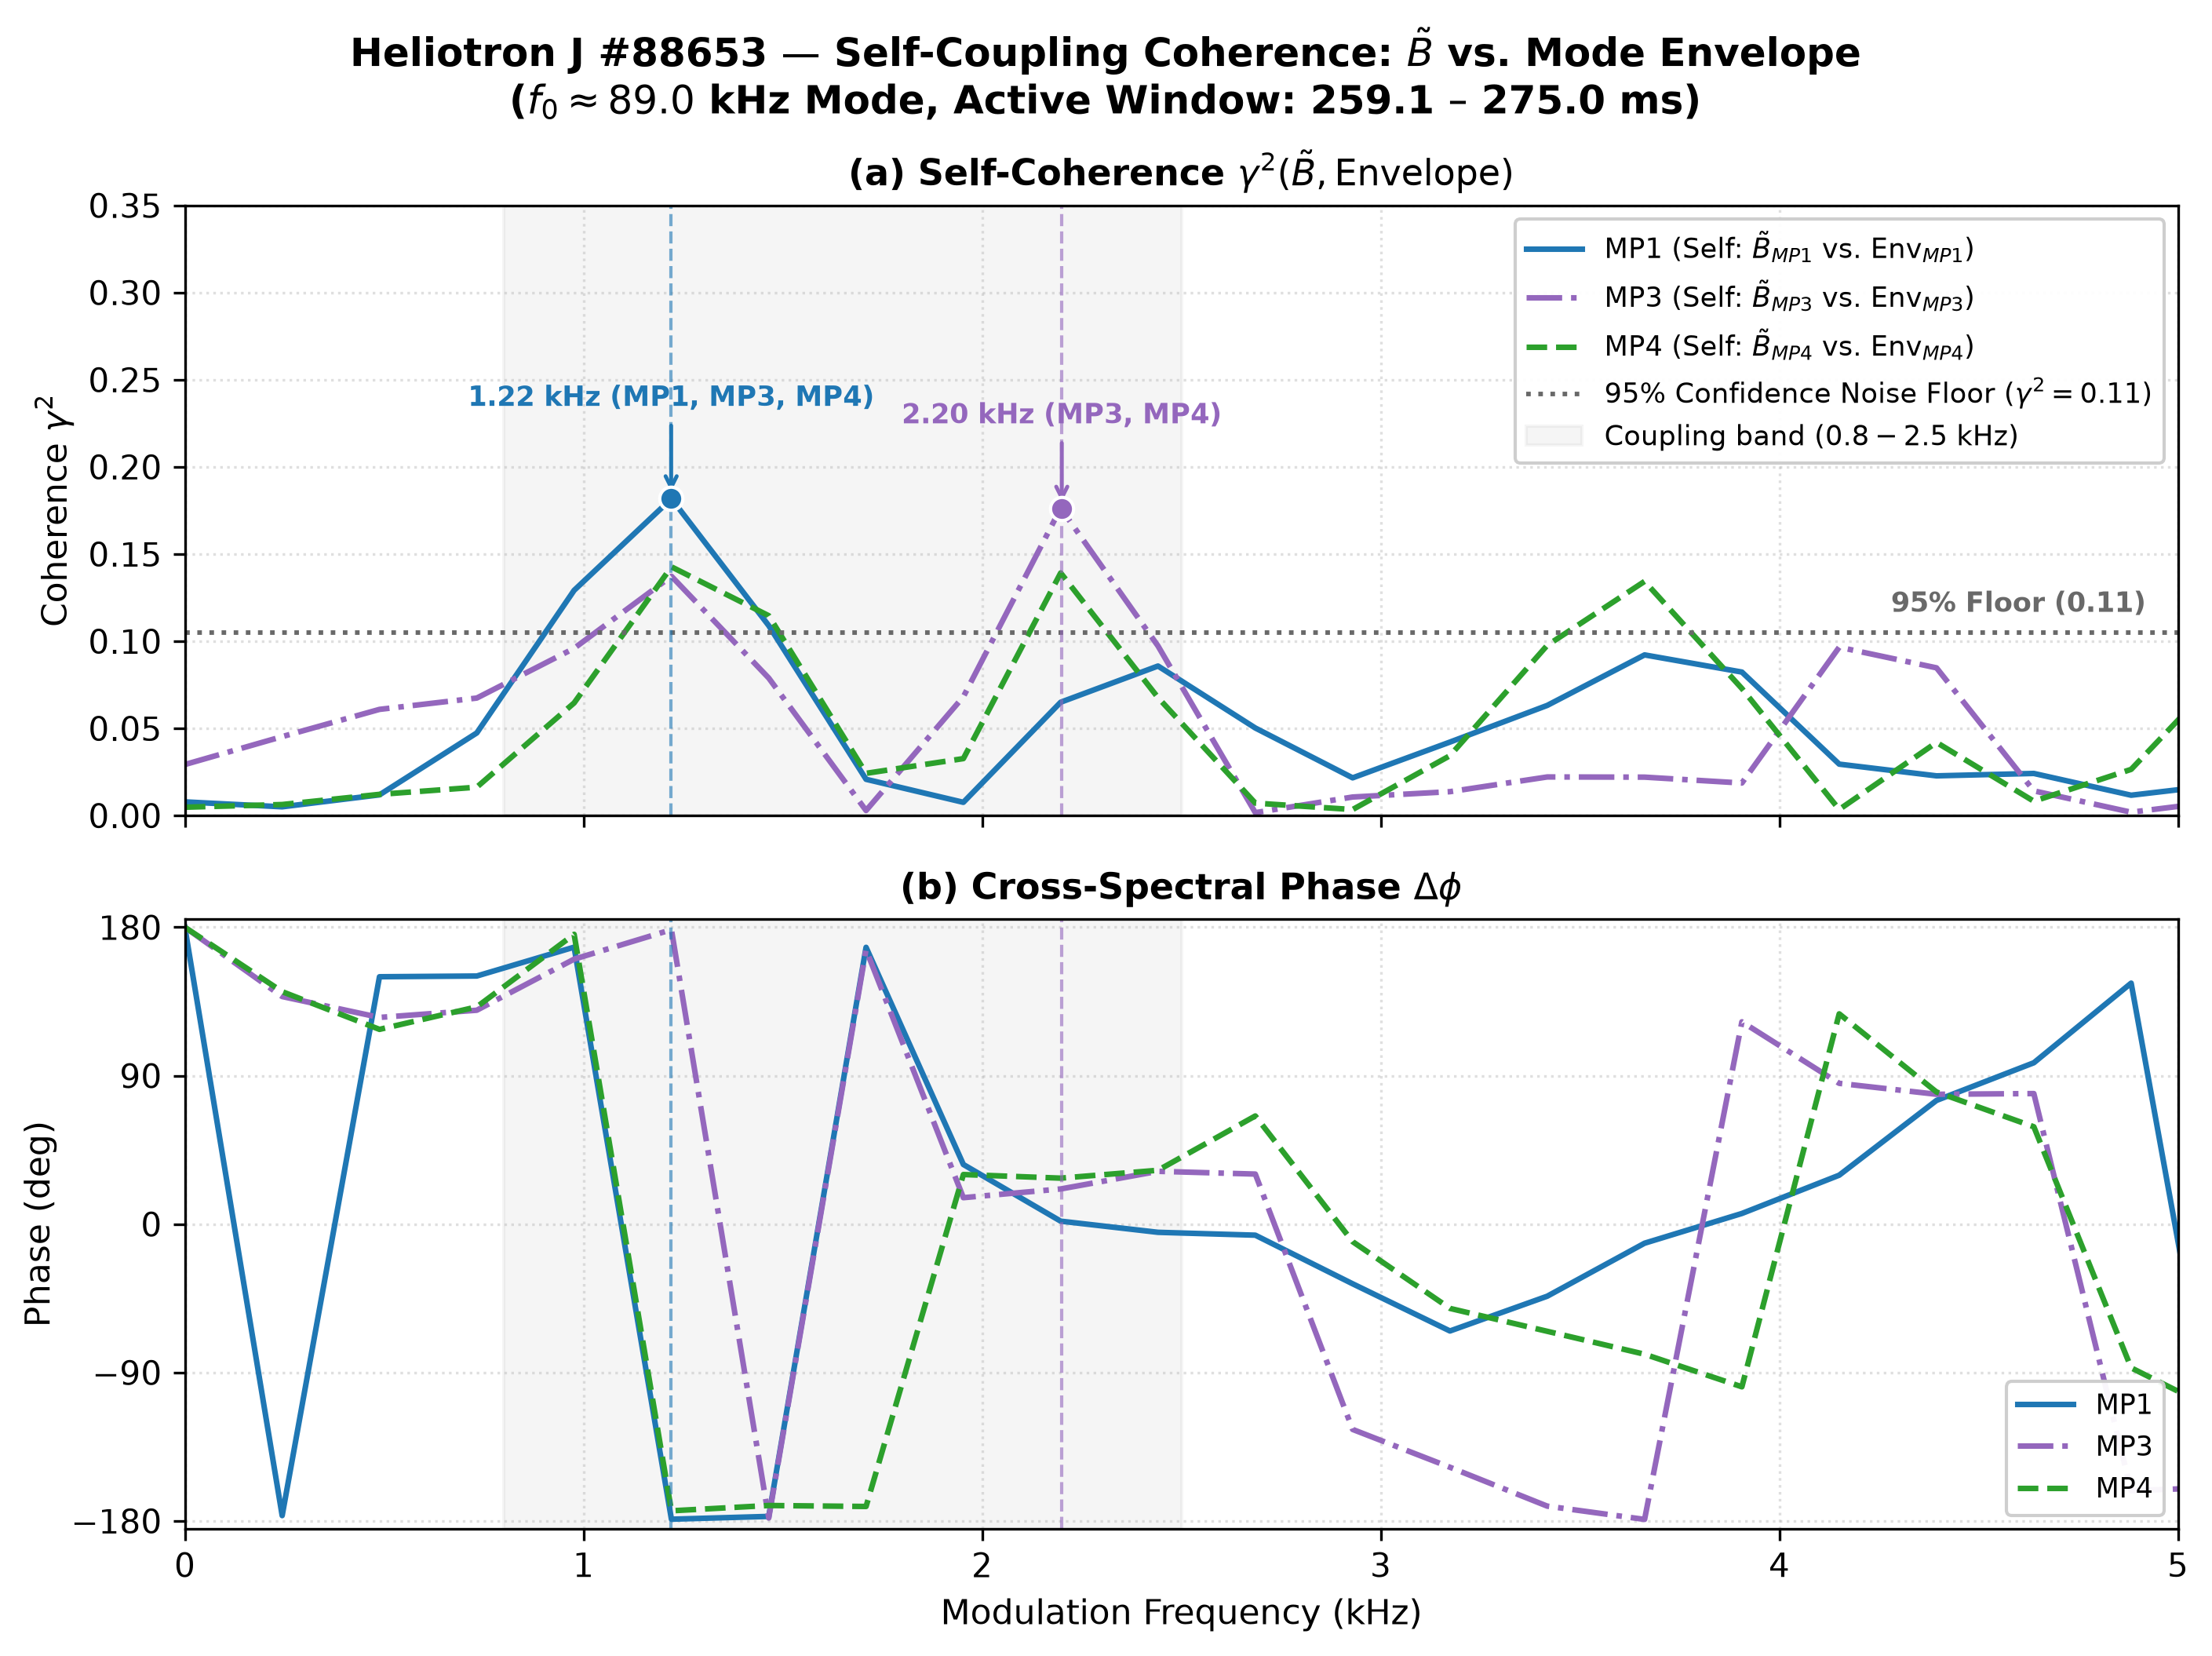
\includegraphics[width=\textwidth]{Images/obj2_dynamics_and_structure/mhd_self_coupling_coherence_shot_88653.png}
        \end{column}
        \begin{column}{0.40\textwidth}
            \footnotesize
            \begin{itemize}
                \item Self-coherence $\gamma^2$ of $\tilde{B}$ with its own Hilbert envelope
                peaks near \SI{1.2}{kHz} (all three probes: MP1 0.18, MP3/MP4 0.14) and
                \SI{2.2}{kHz} (MP3 0.18, MP4 0.14; MP1 below floor), above the
                nominal 95\% floor of 0.105 (\SIrange{259.1}{275.0}{ms}; segment overlap makes
                the floor optimistic).
                \item The \SI{2.2}{kHz} peak (MP3, MP4) persists at 2$\times$ and 4$\times$
                resolution and exceeds the floor in all three probes in the NBI-only window; the
                \SI{1.2}{kHz} peak already clears the floor on all three probes here, strongest
                on MP1.
                \item Consistent with a weak wave--envelope interaction (linear beating of
                adjacent lines also gives envelope coherence); motivation for Objective 3.
            \end{itemize}
        \end{column}
    \end{columns}
\end{frame}

\begin{frame}{Backup: Objective 2 -- Secondary Band Macroscopic Correlations}
    \begin{figure}[h!]
        \centering
        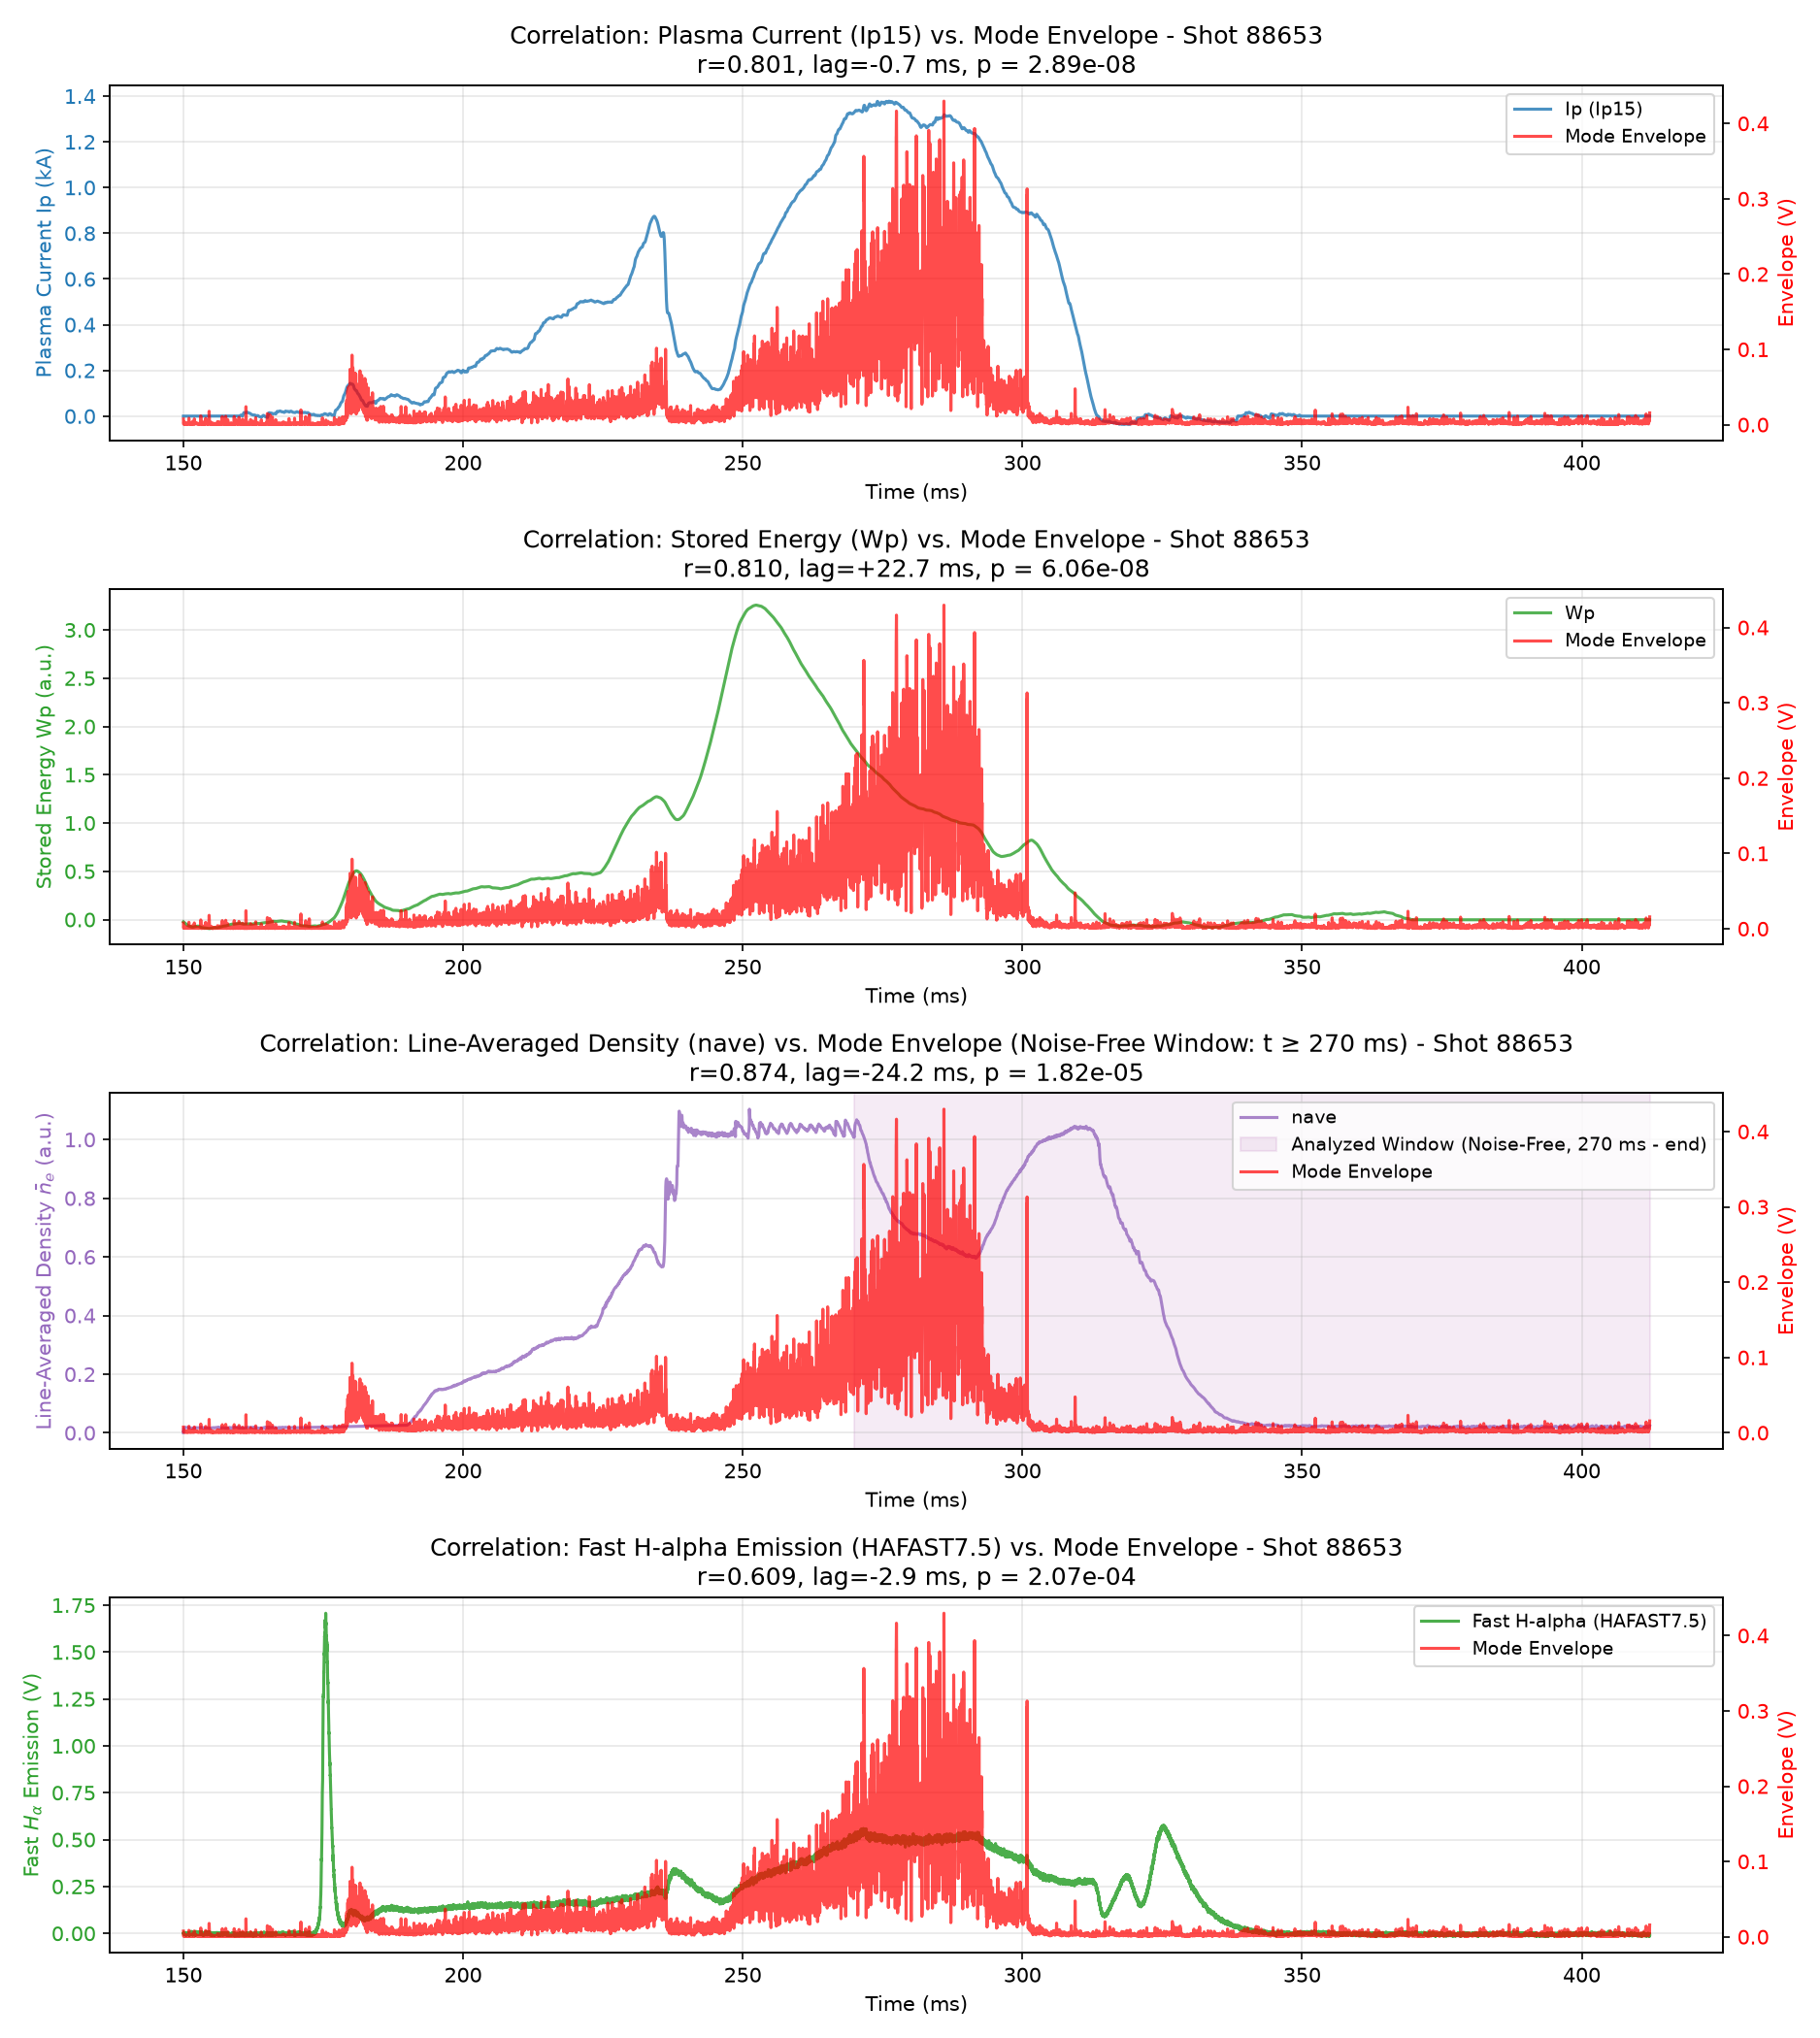
\includegraphics[height=0.85\textheight]{Images/obj2_dynamics_and_structure/mhd_analysis_objective2_88653_40_80kHz.png}
    \end{figure}
\end{frame}

\begin{frame}{Backup: Objective 2 -- Secondary Band Heating Synchronization}
    \begin{figure}[h!]
        \centering
        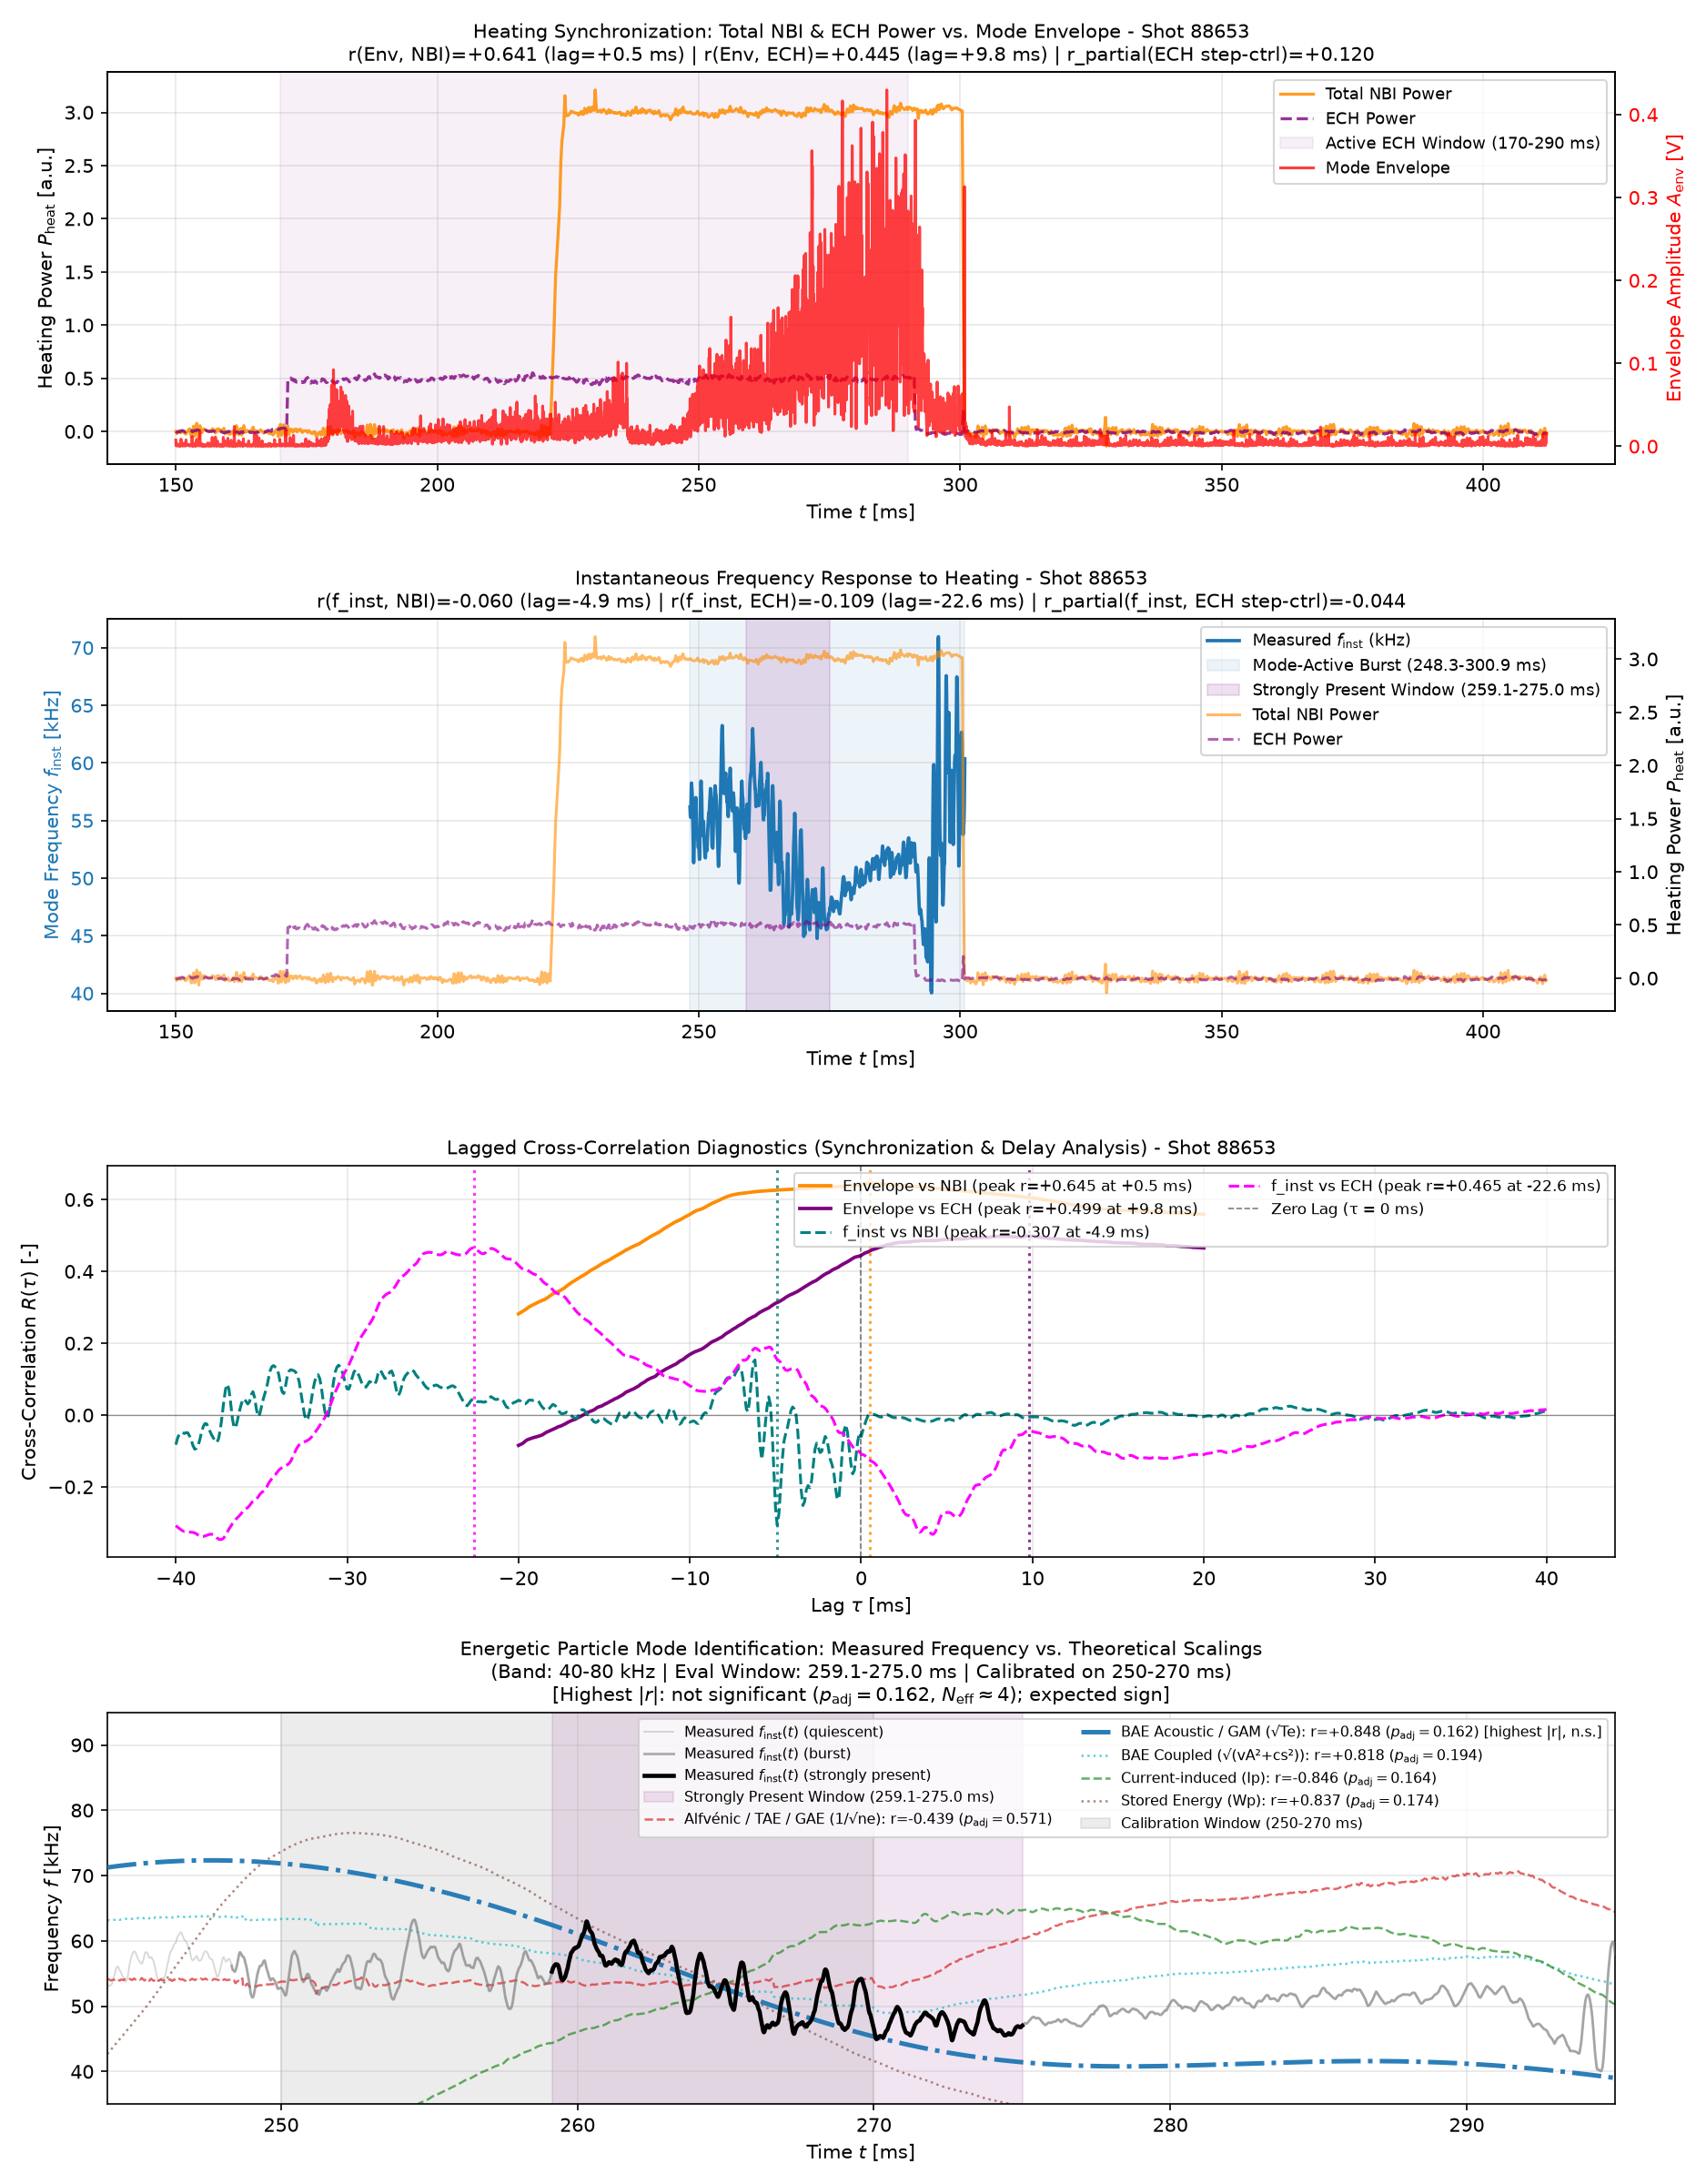
\includegraphics[height=0.85\textheight]{Images/obj2_dynamics_and_structure/mhd_analysis_objective2_heating_88653_40_80kHz.png}
    \end{figure}
\end{frame}

\begin{frame}{Backup: Objective 2 -- Primary Band Macroscopic Correlations}
    \begin{figure}[h!]
        \centering
        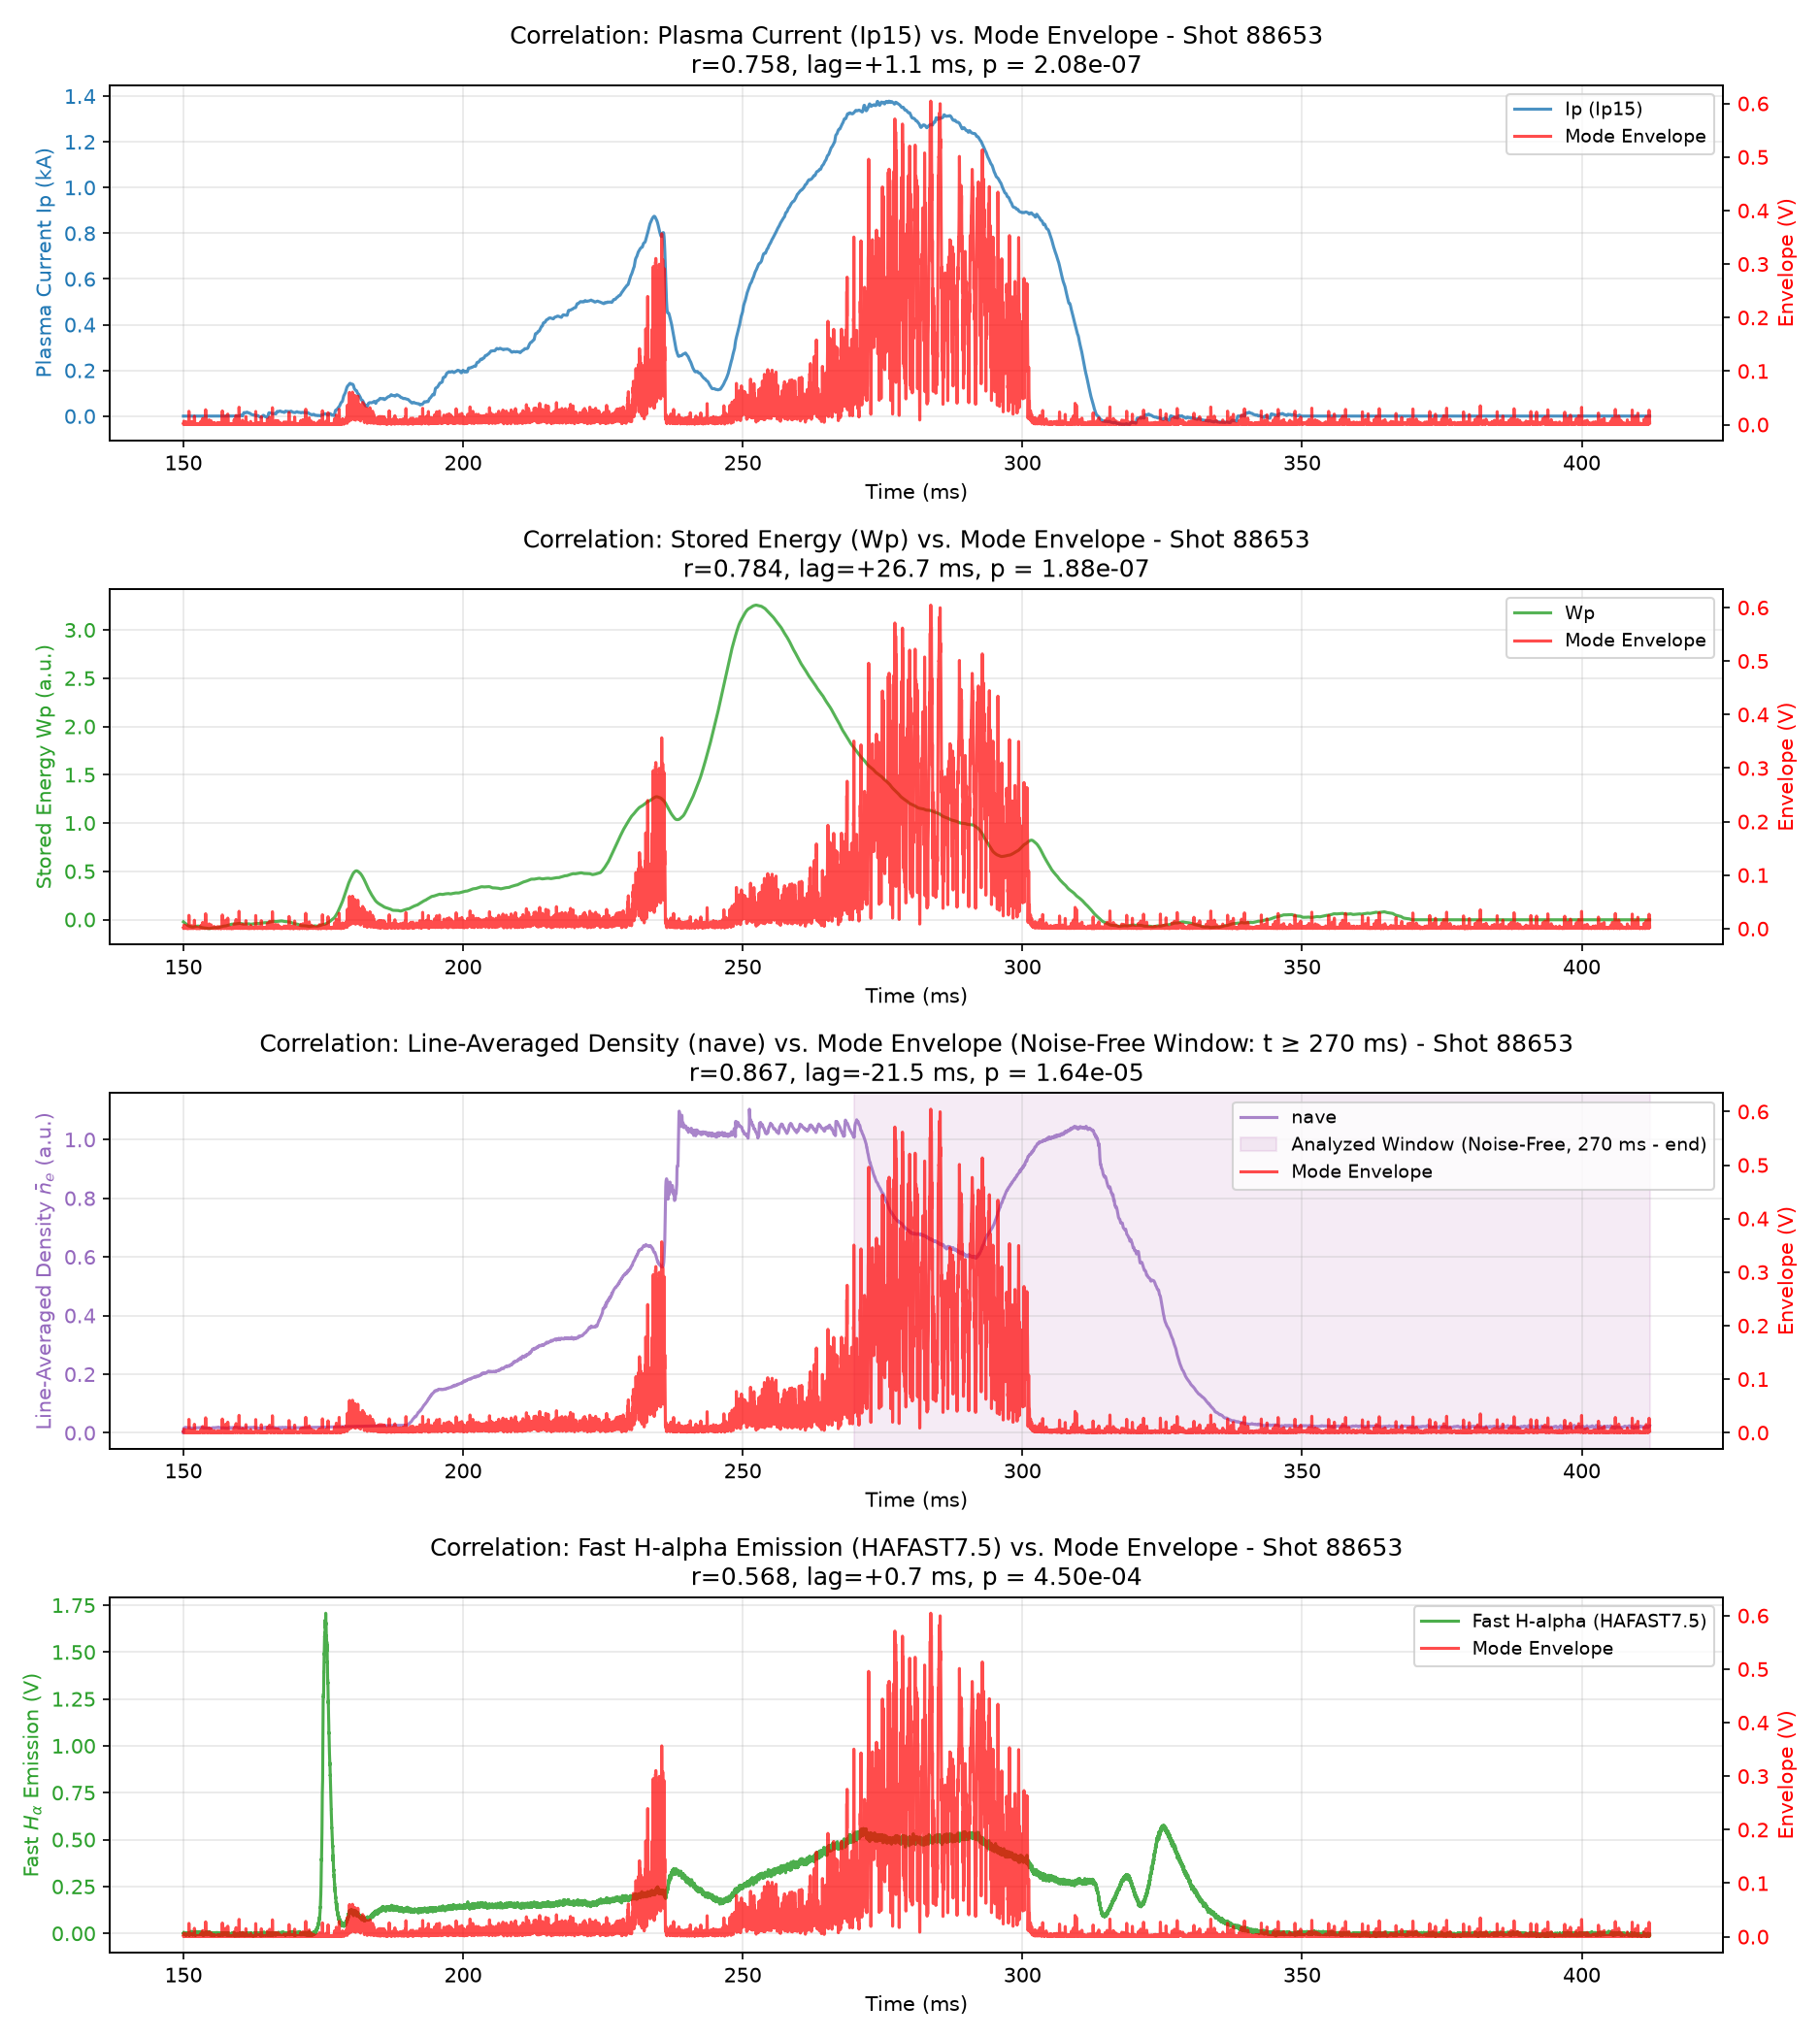
\includegraphics[height=0.85\textheight]{Images/obj2_dynamics_and_structure/mhd_analysis_objective2_88653_80_120kHz.png}
    \end{figure}
\end{frame}

\begin{frame}{Backup: Objective 2 -- Primary Band Heating Synchronization}
    \begin{figure}[h!]
        \centering
        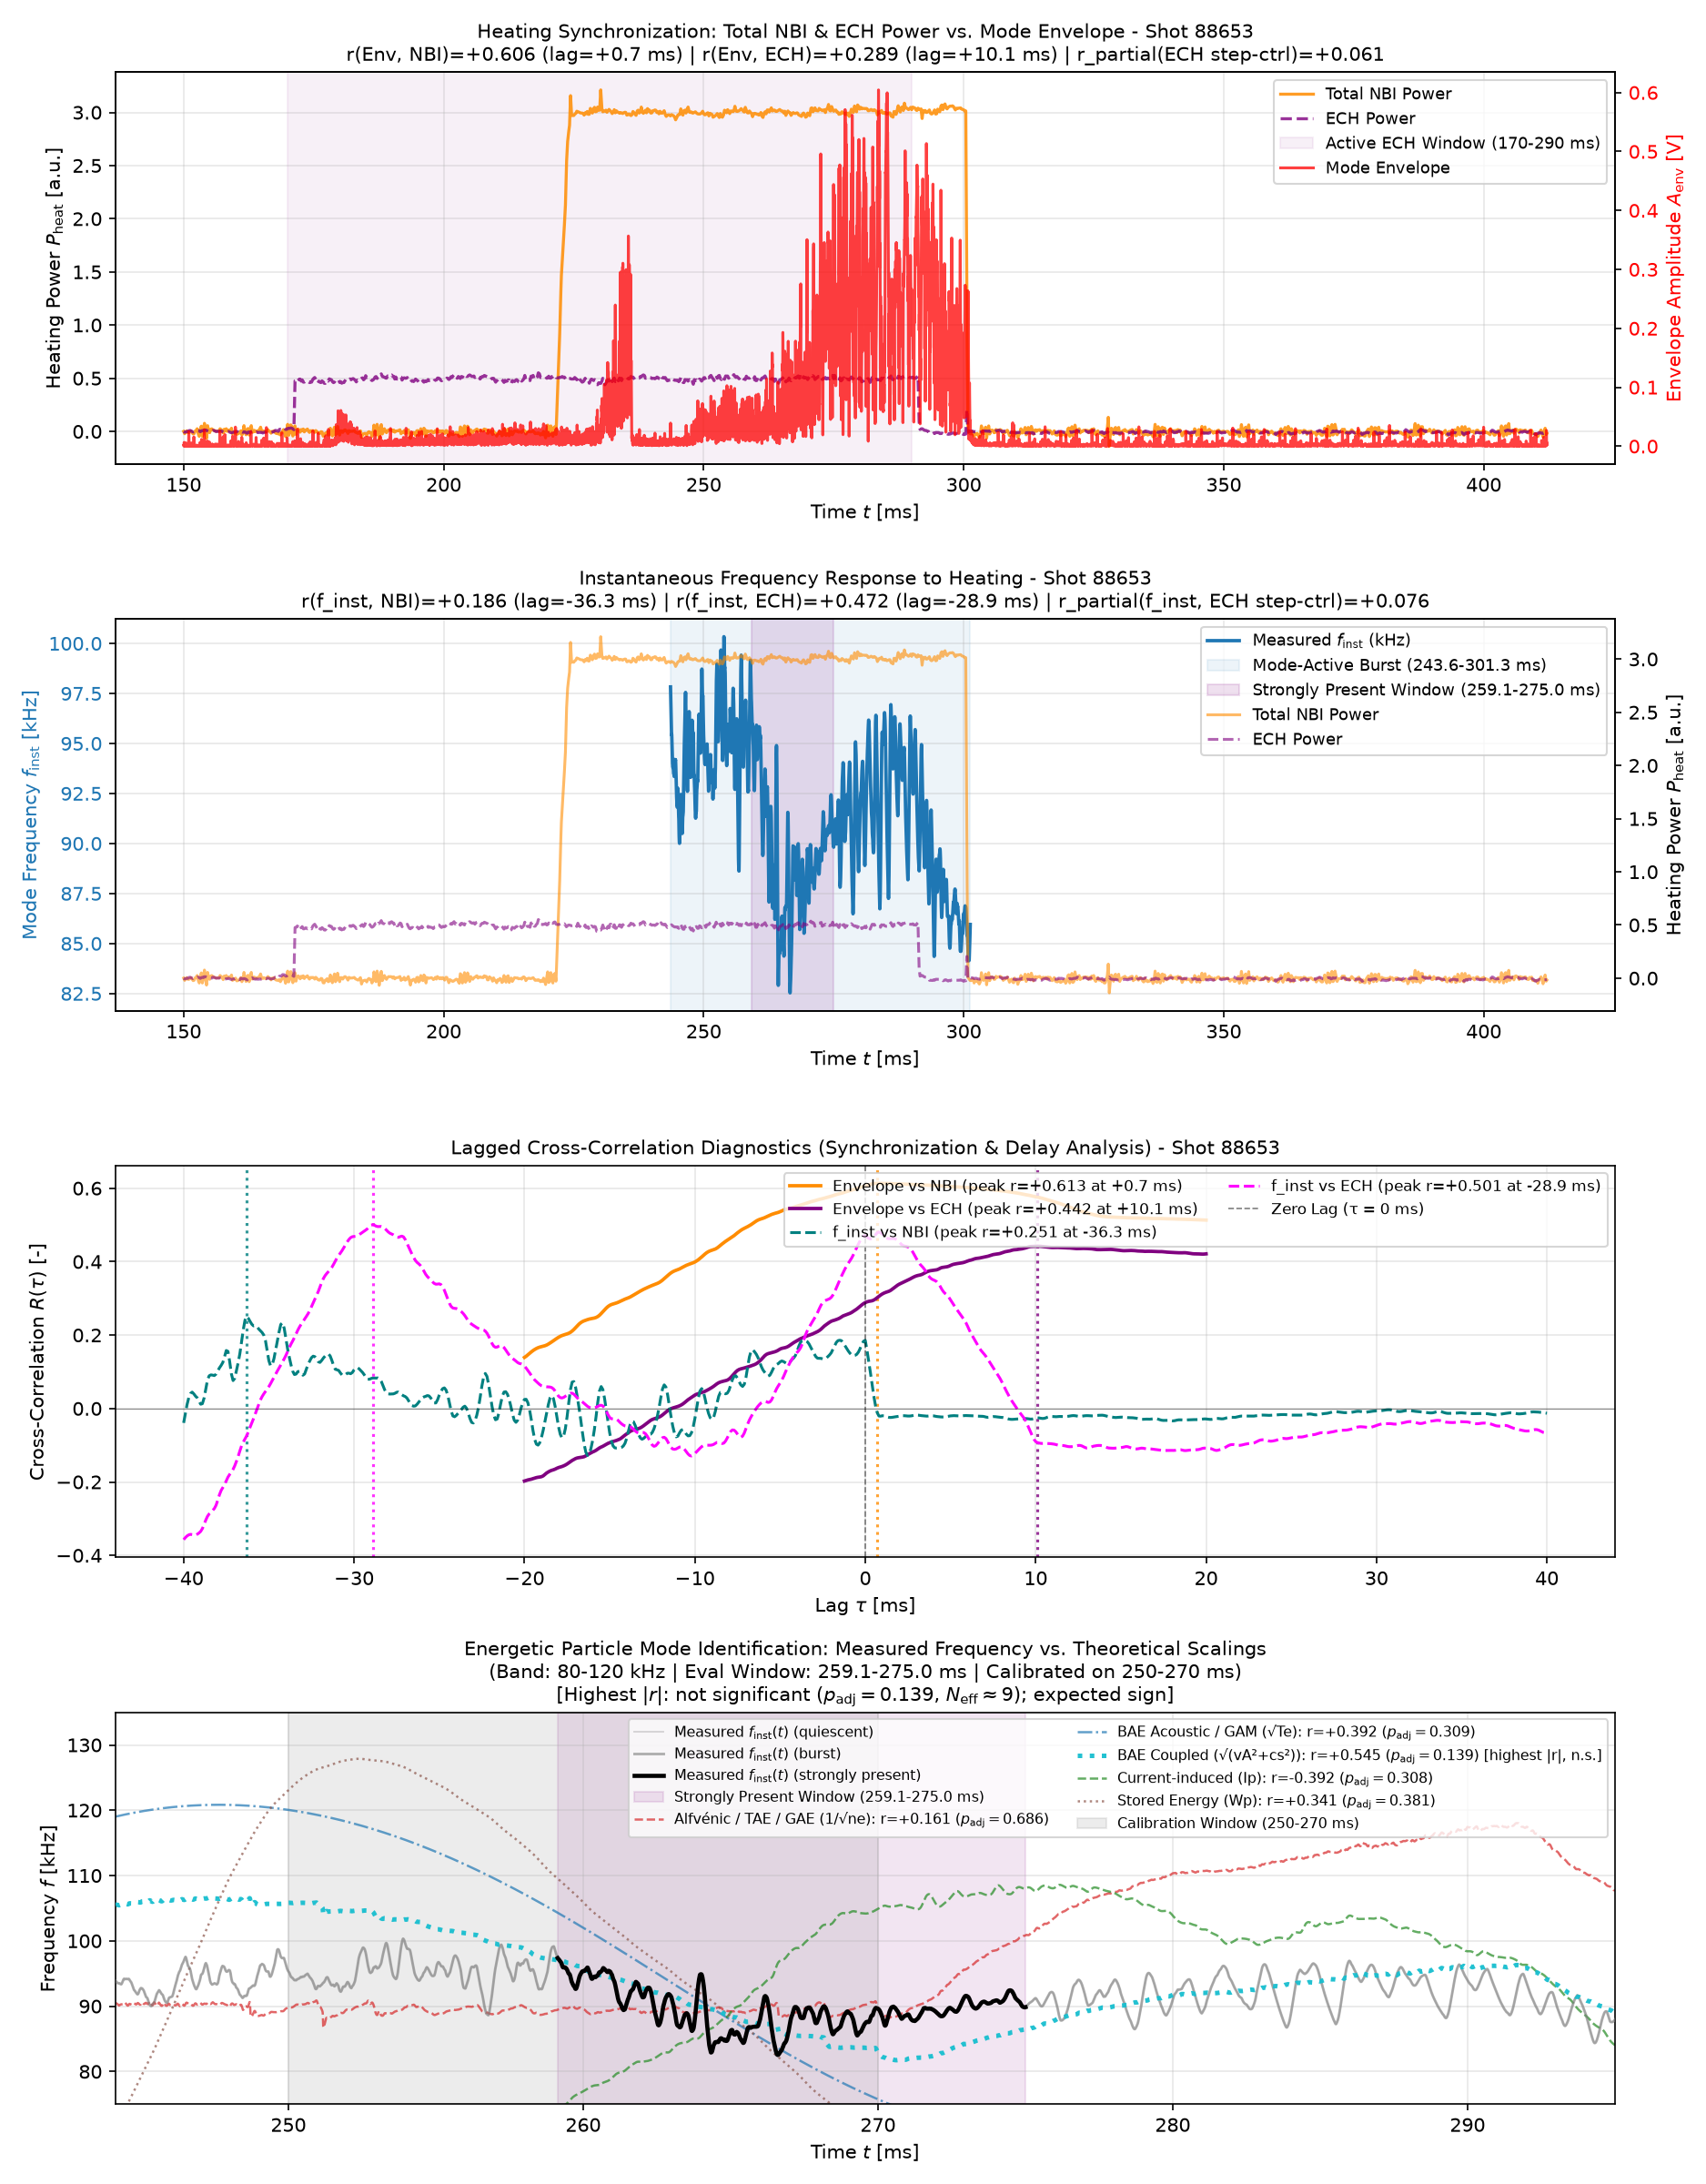
\includegraphics[height=0.85\textheight]{Images/obj2_dynamics_and_structure/mhd_analysis_objective2_heating_88653_80_120kHz.png}
    \end{figure}
\end{frame}

\begin{frame}{Backup: Objective 2 -- Secondary Band Poloidal Structure (Full Window)}
    \begin{figure}[h!]
        \centering
        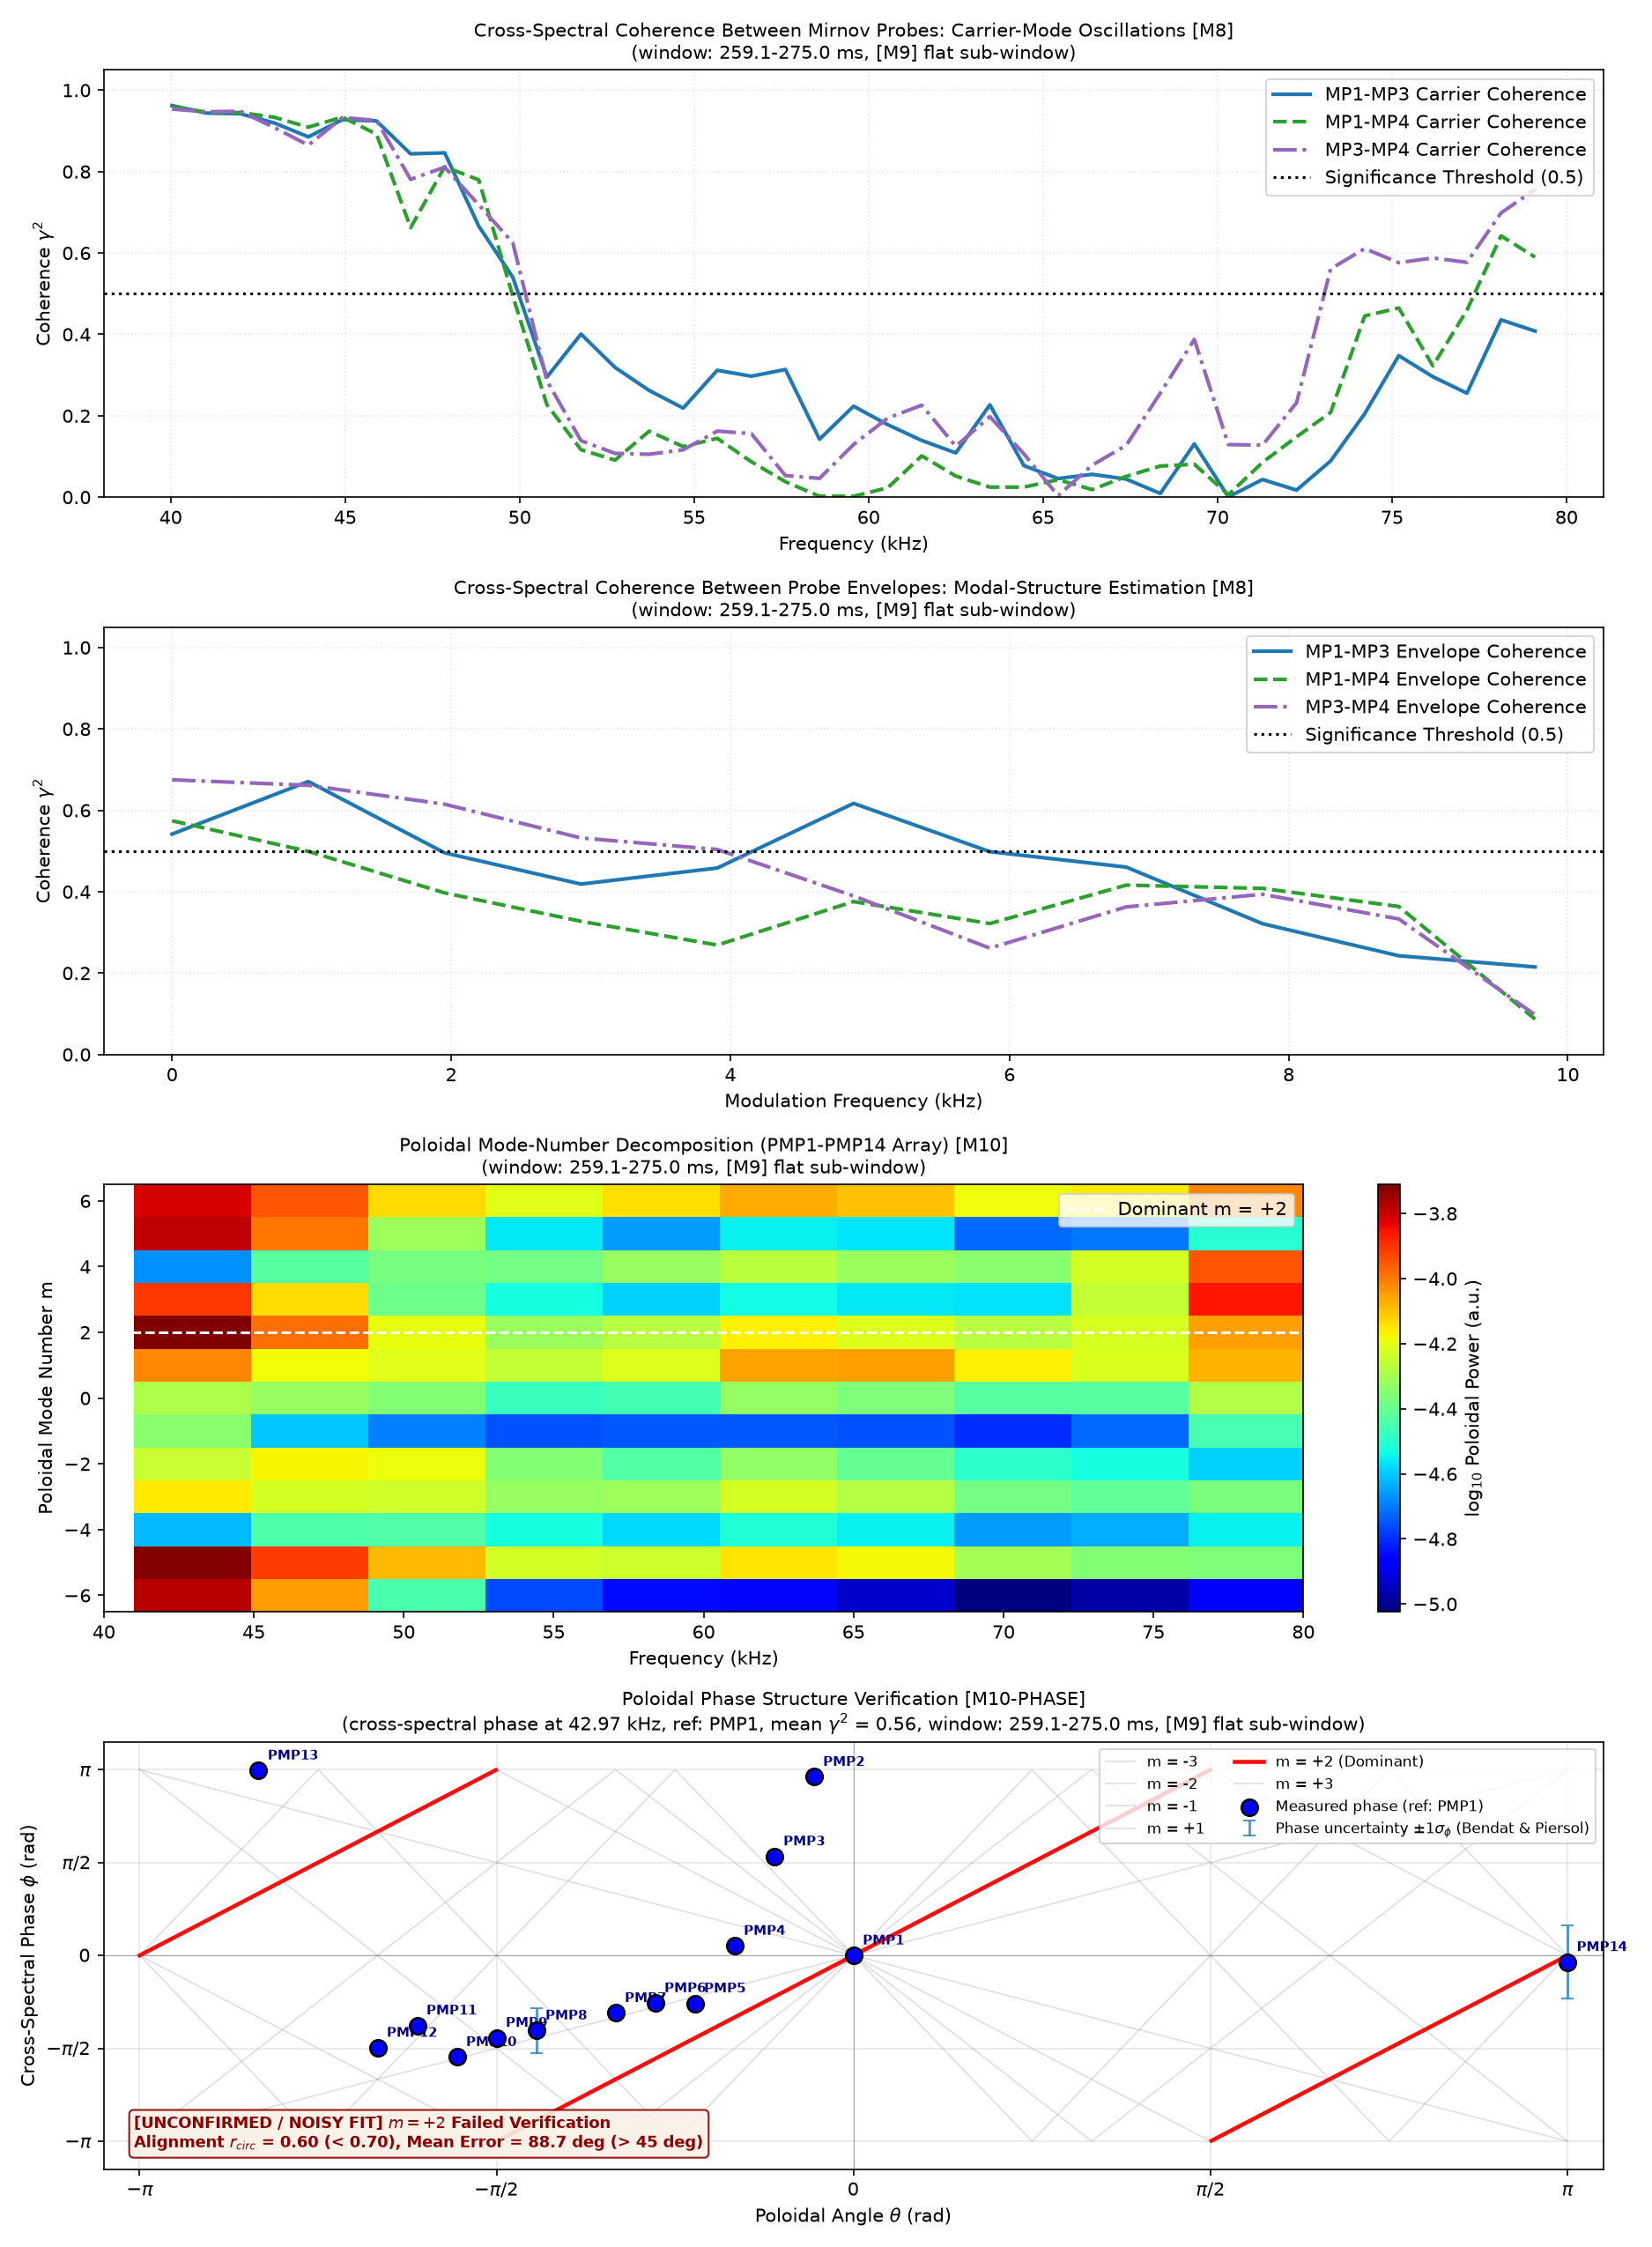
\includegraphics[width=0.85\textwidth,height=0.62\textheight,keepaspectratio]{Images/obj2_dynamics_and_structure/mhd_analysis_objective2_structure_88653_40_80kHz.png}
    \end{figure}
    \footnotesize
    Full ECH+NBI window (\SIrange{259.1}{291.3}{ms}), companion to the Primary full-window
    structure on the backup ``Two Bands'' slide. Consistent with the tentative status
    reported there: $m$ is not stable across the ECH+NBI/NBI-only split (see next slide).
\end{frame}

\begin{frame}{Backup: Objective 2 Comparative -- Secondary Band Spatial Structure}
    \begin{columns}[T]
        \begin{column}{0.5\textwidth}
            \centering ECH+NBI\\
            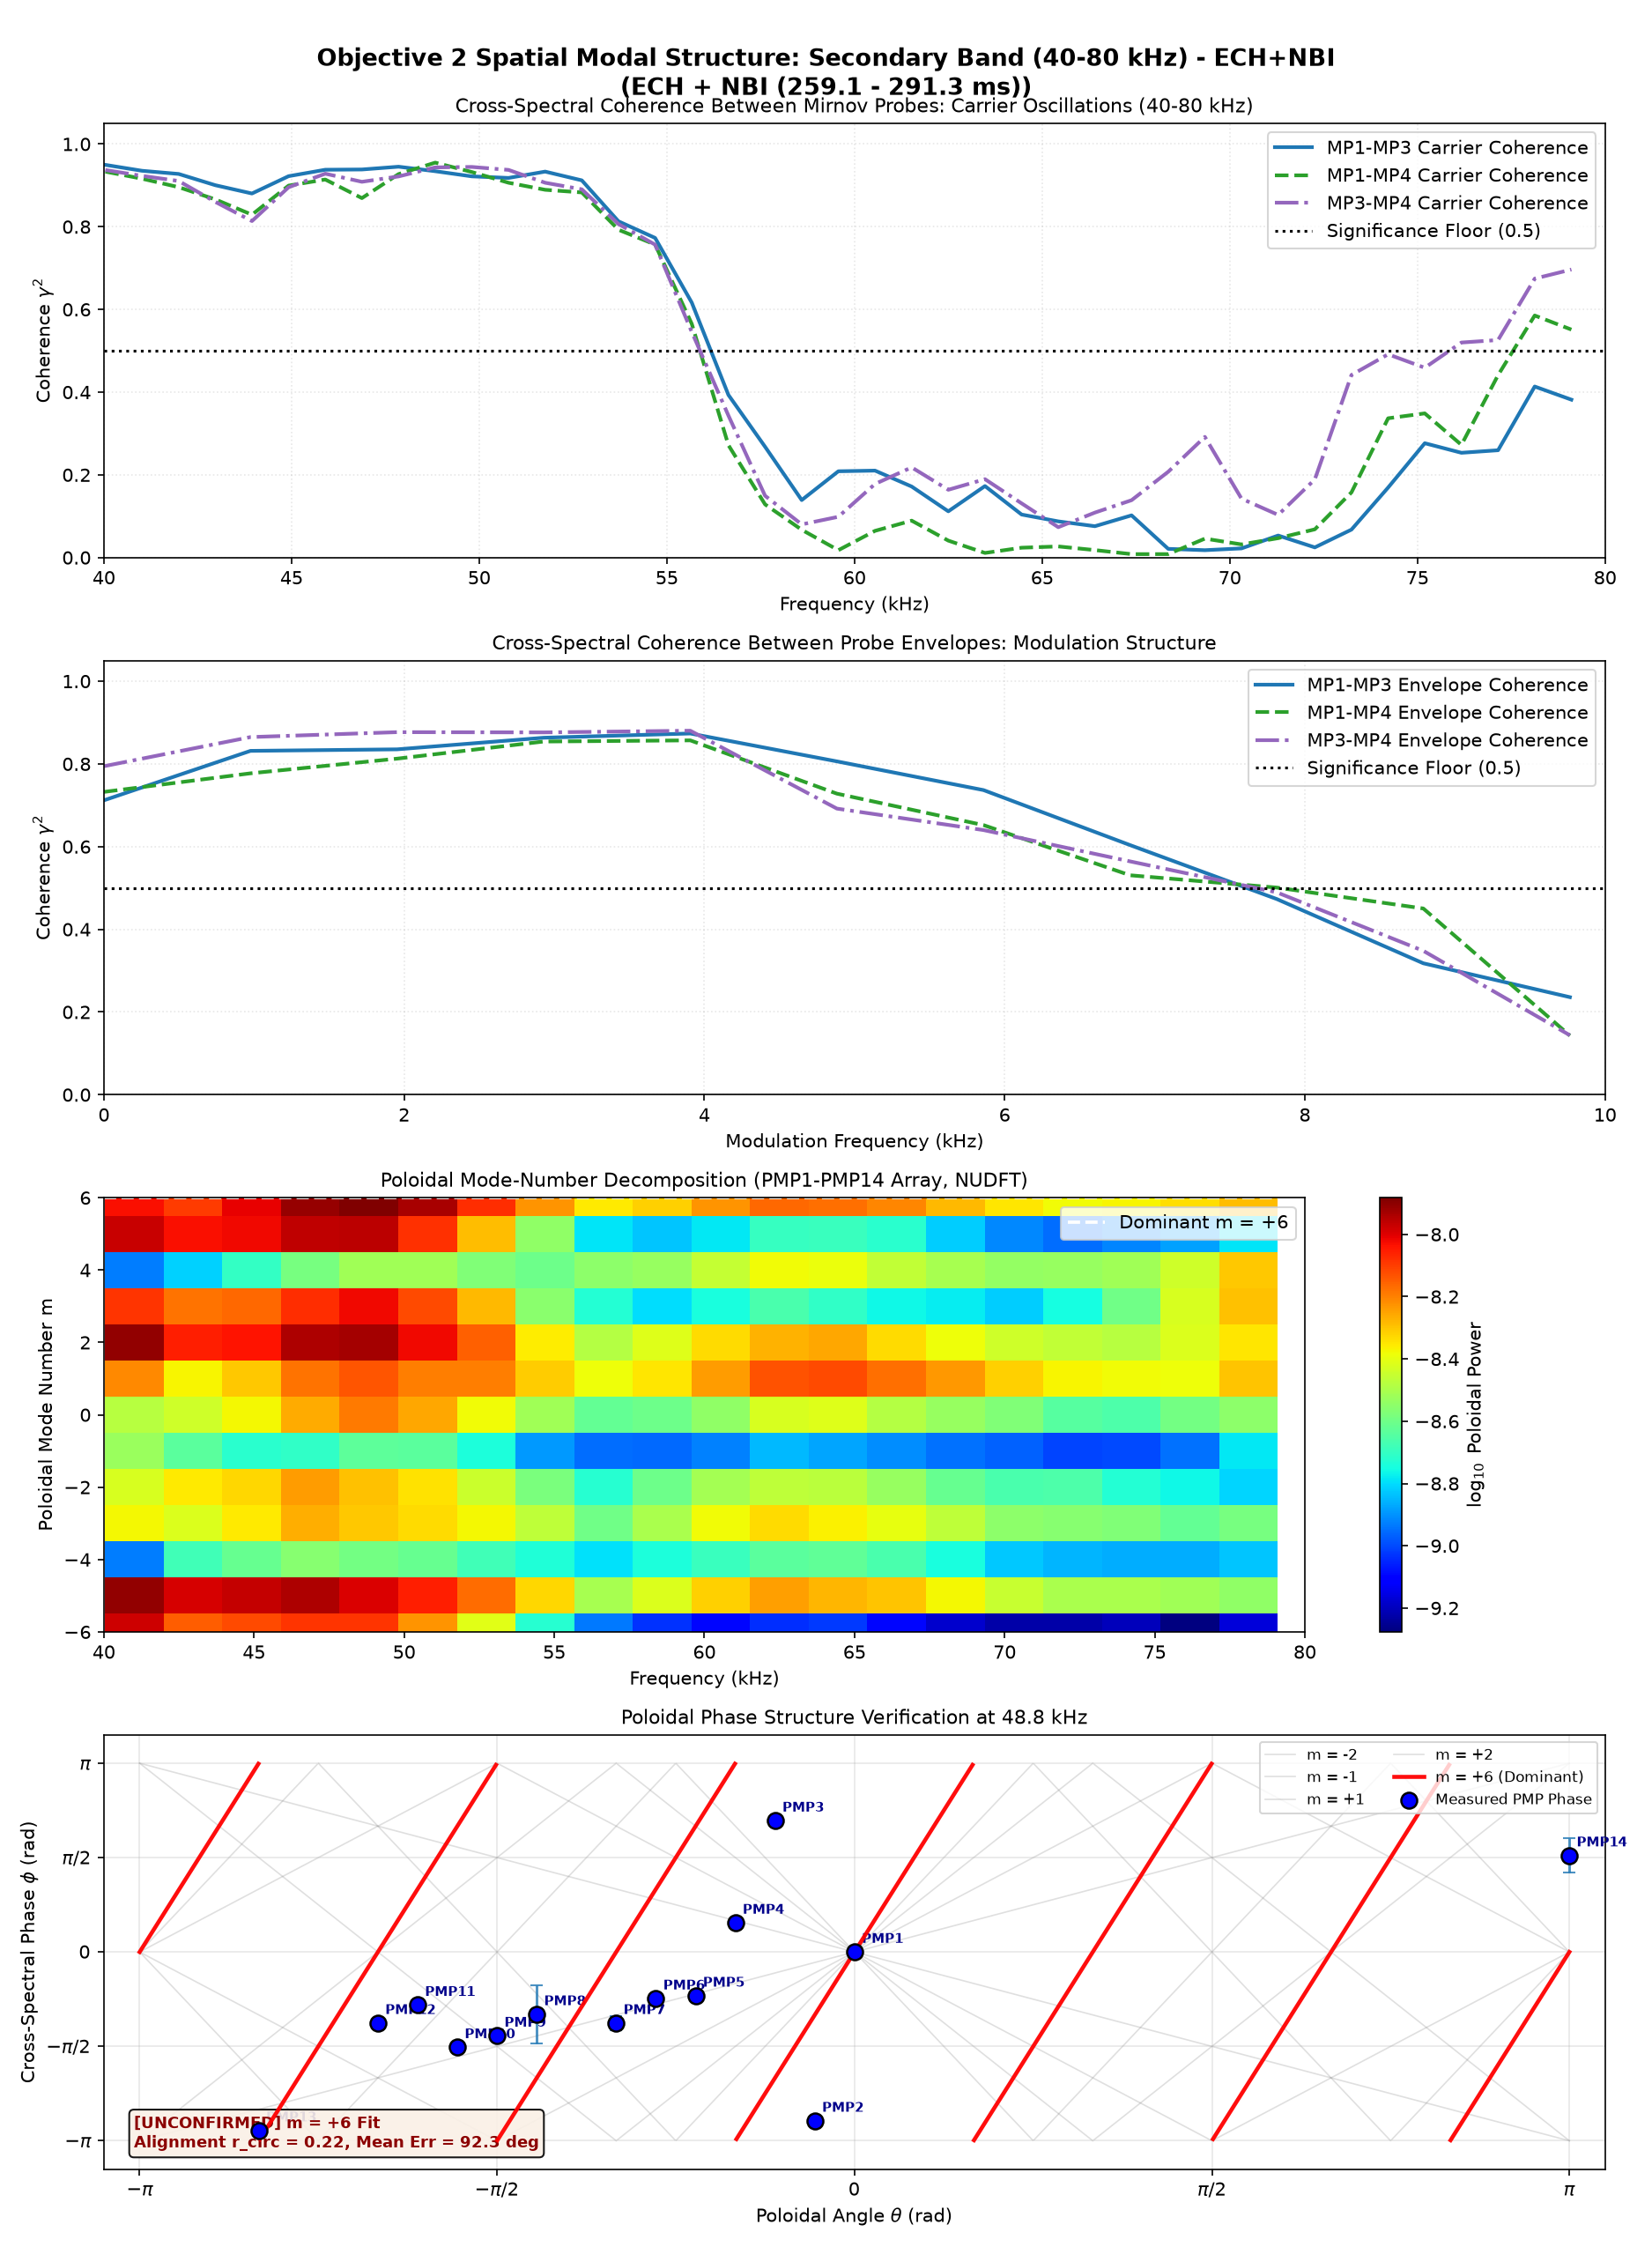
\includegraphics[width=\textwidth,height=0.66\textheight,keepaspectratio]{Images/heating_phase_comparison/mhd_analysis_objective2_structure_88653_40_80kHz_ECH_NBI.png}
        \end{column}
        \begin{column}{0.5\textwidth}
            \centering NBI-only\\
            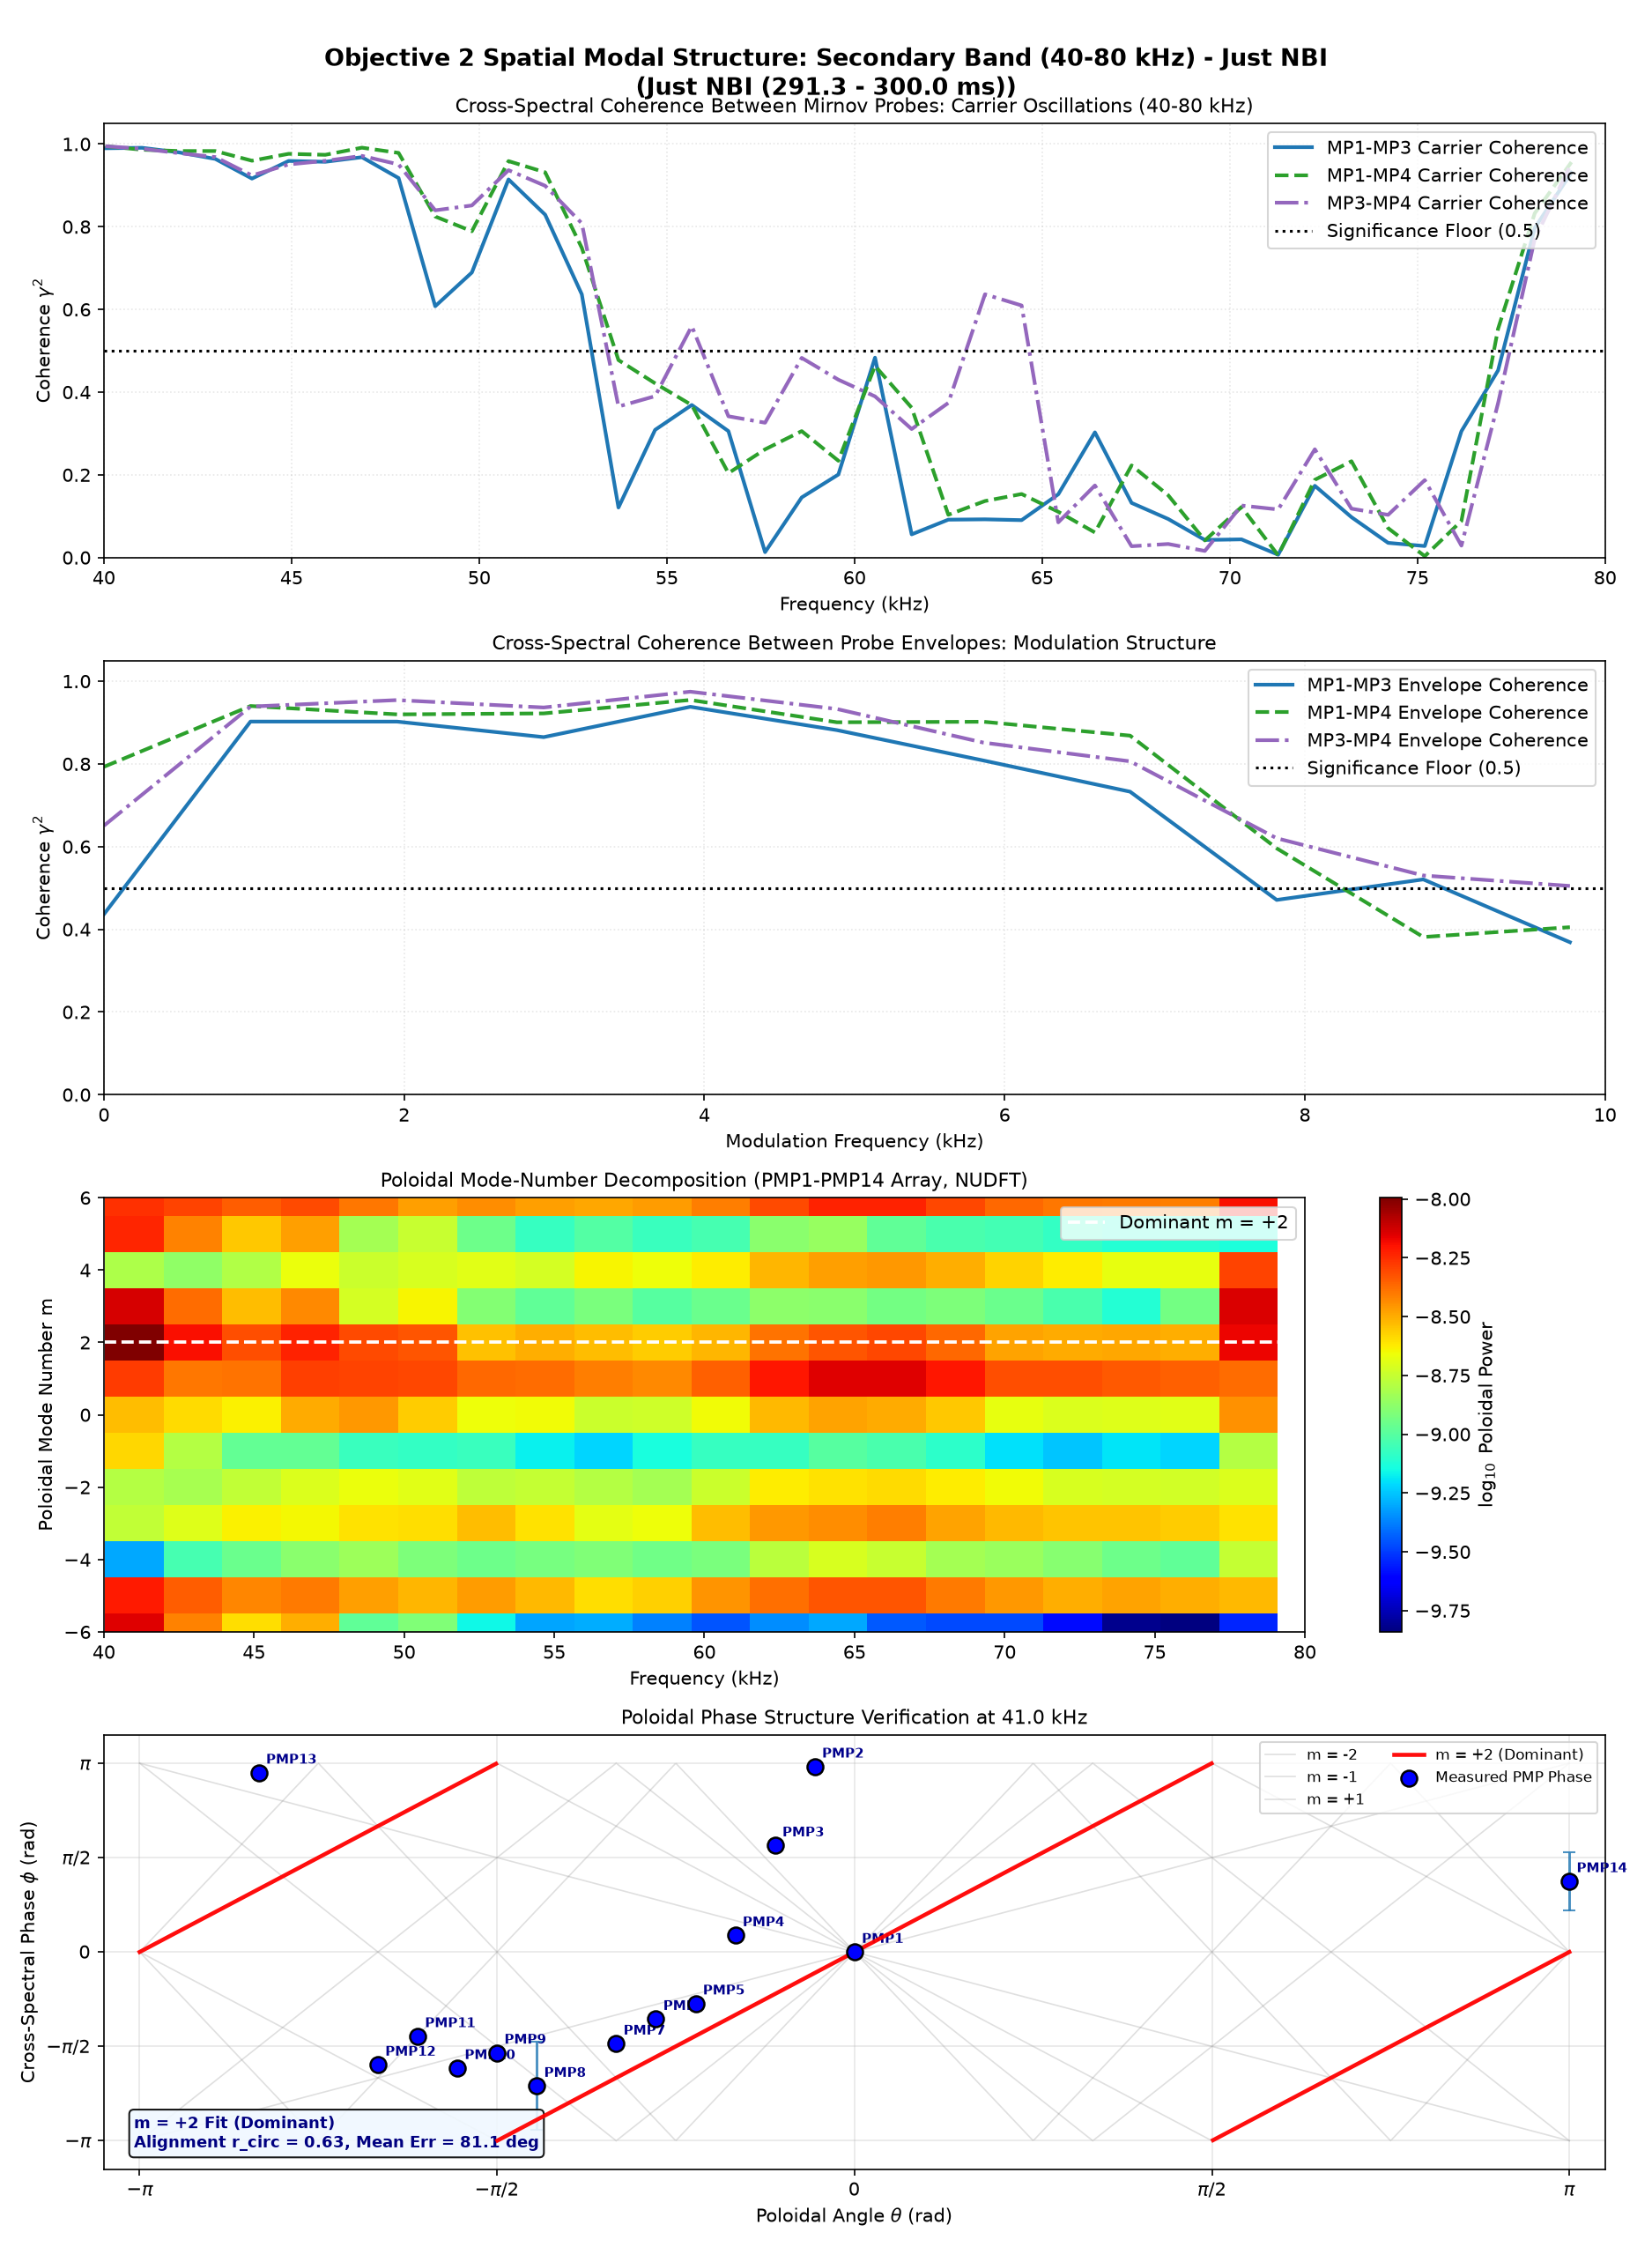
\includegraphics[width=\textwidth,height=0.66\textheight,keepaspectratio]{Images/heating_phase_comparison/mhd_analysis_objective2_structure_88653_40_80kHz_NBI_only.png}
        \end{column}
    \end{columns}
\end{frame}

\begin{frame}{Backup: Objective 2 Comparative -- Primary Band Spatial Structure}
    \begin{columns}[T]
        \begin{column}{0.5\textwidth}
            \centering ECH+NBI\\
            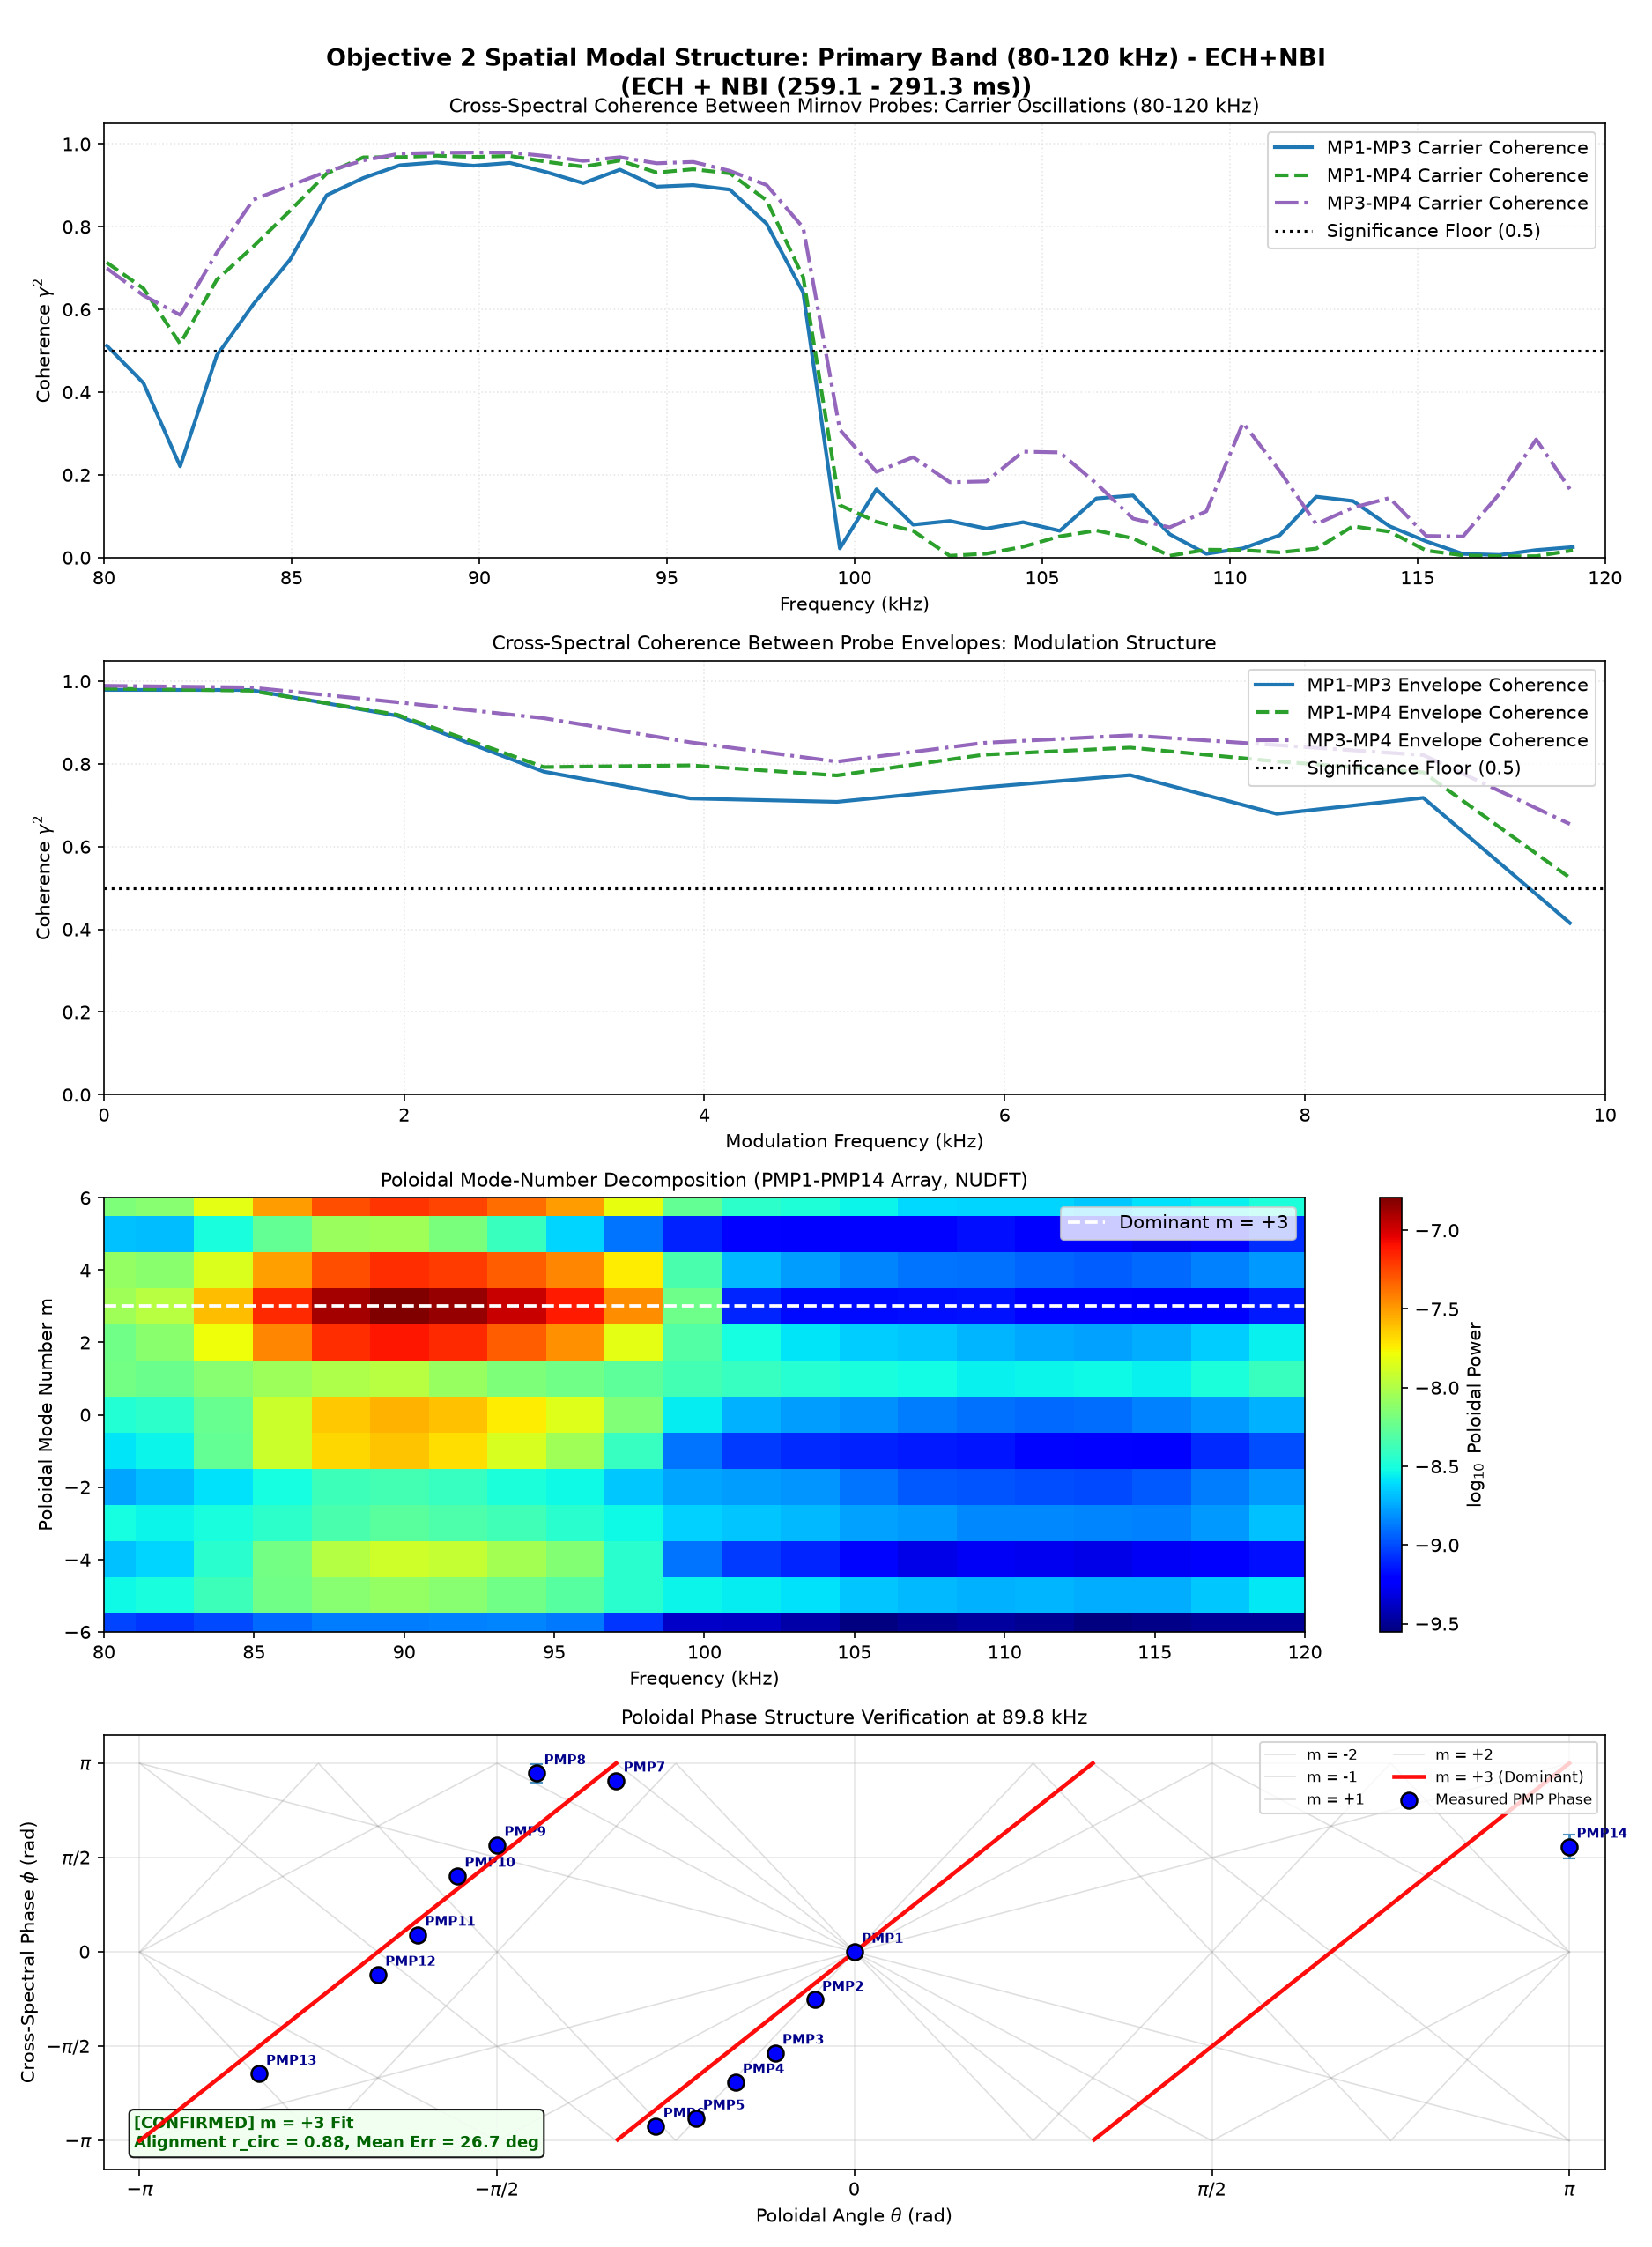
\includegraphics[width=\textwidth,height=0.66\textheight,keepaspectratio]{Images/heating_phase_comparison/mhd_analysis_objective2_structure_88653_80_120kHz_ECH_NBI.png}
        \end{column}
        \begin{column}{0.5\textwidth}
            \centering NBI-only\\
            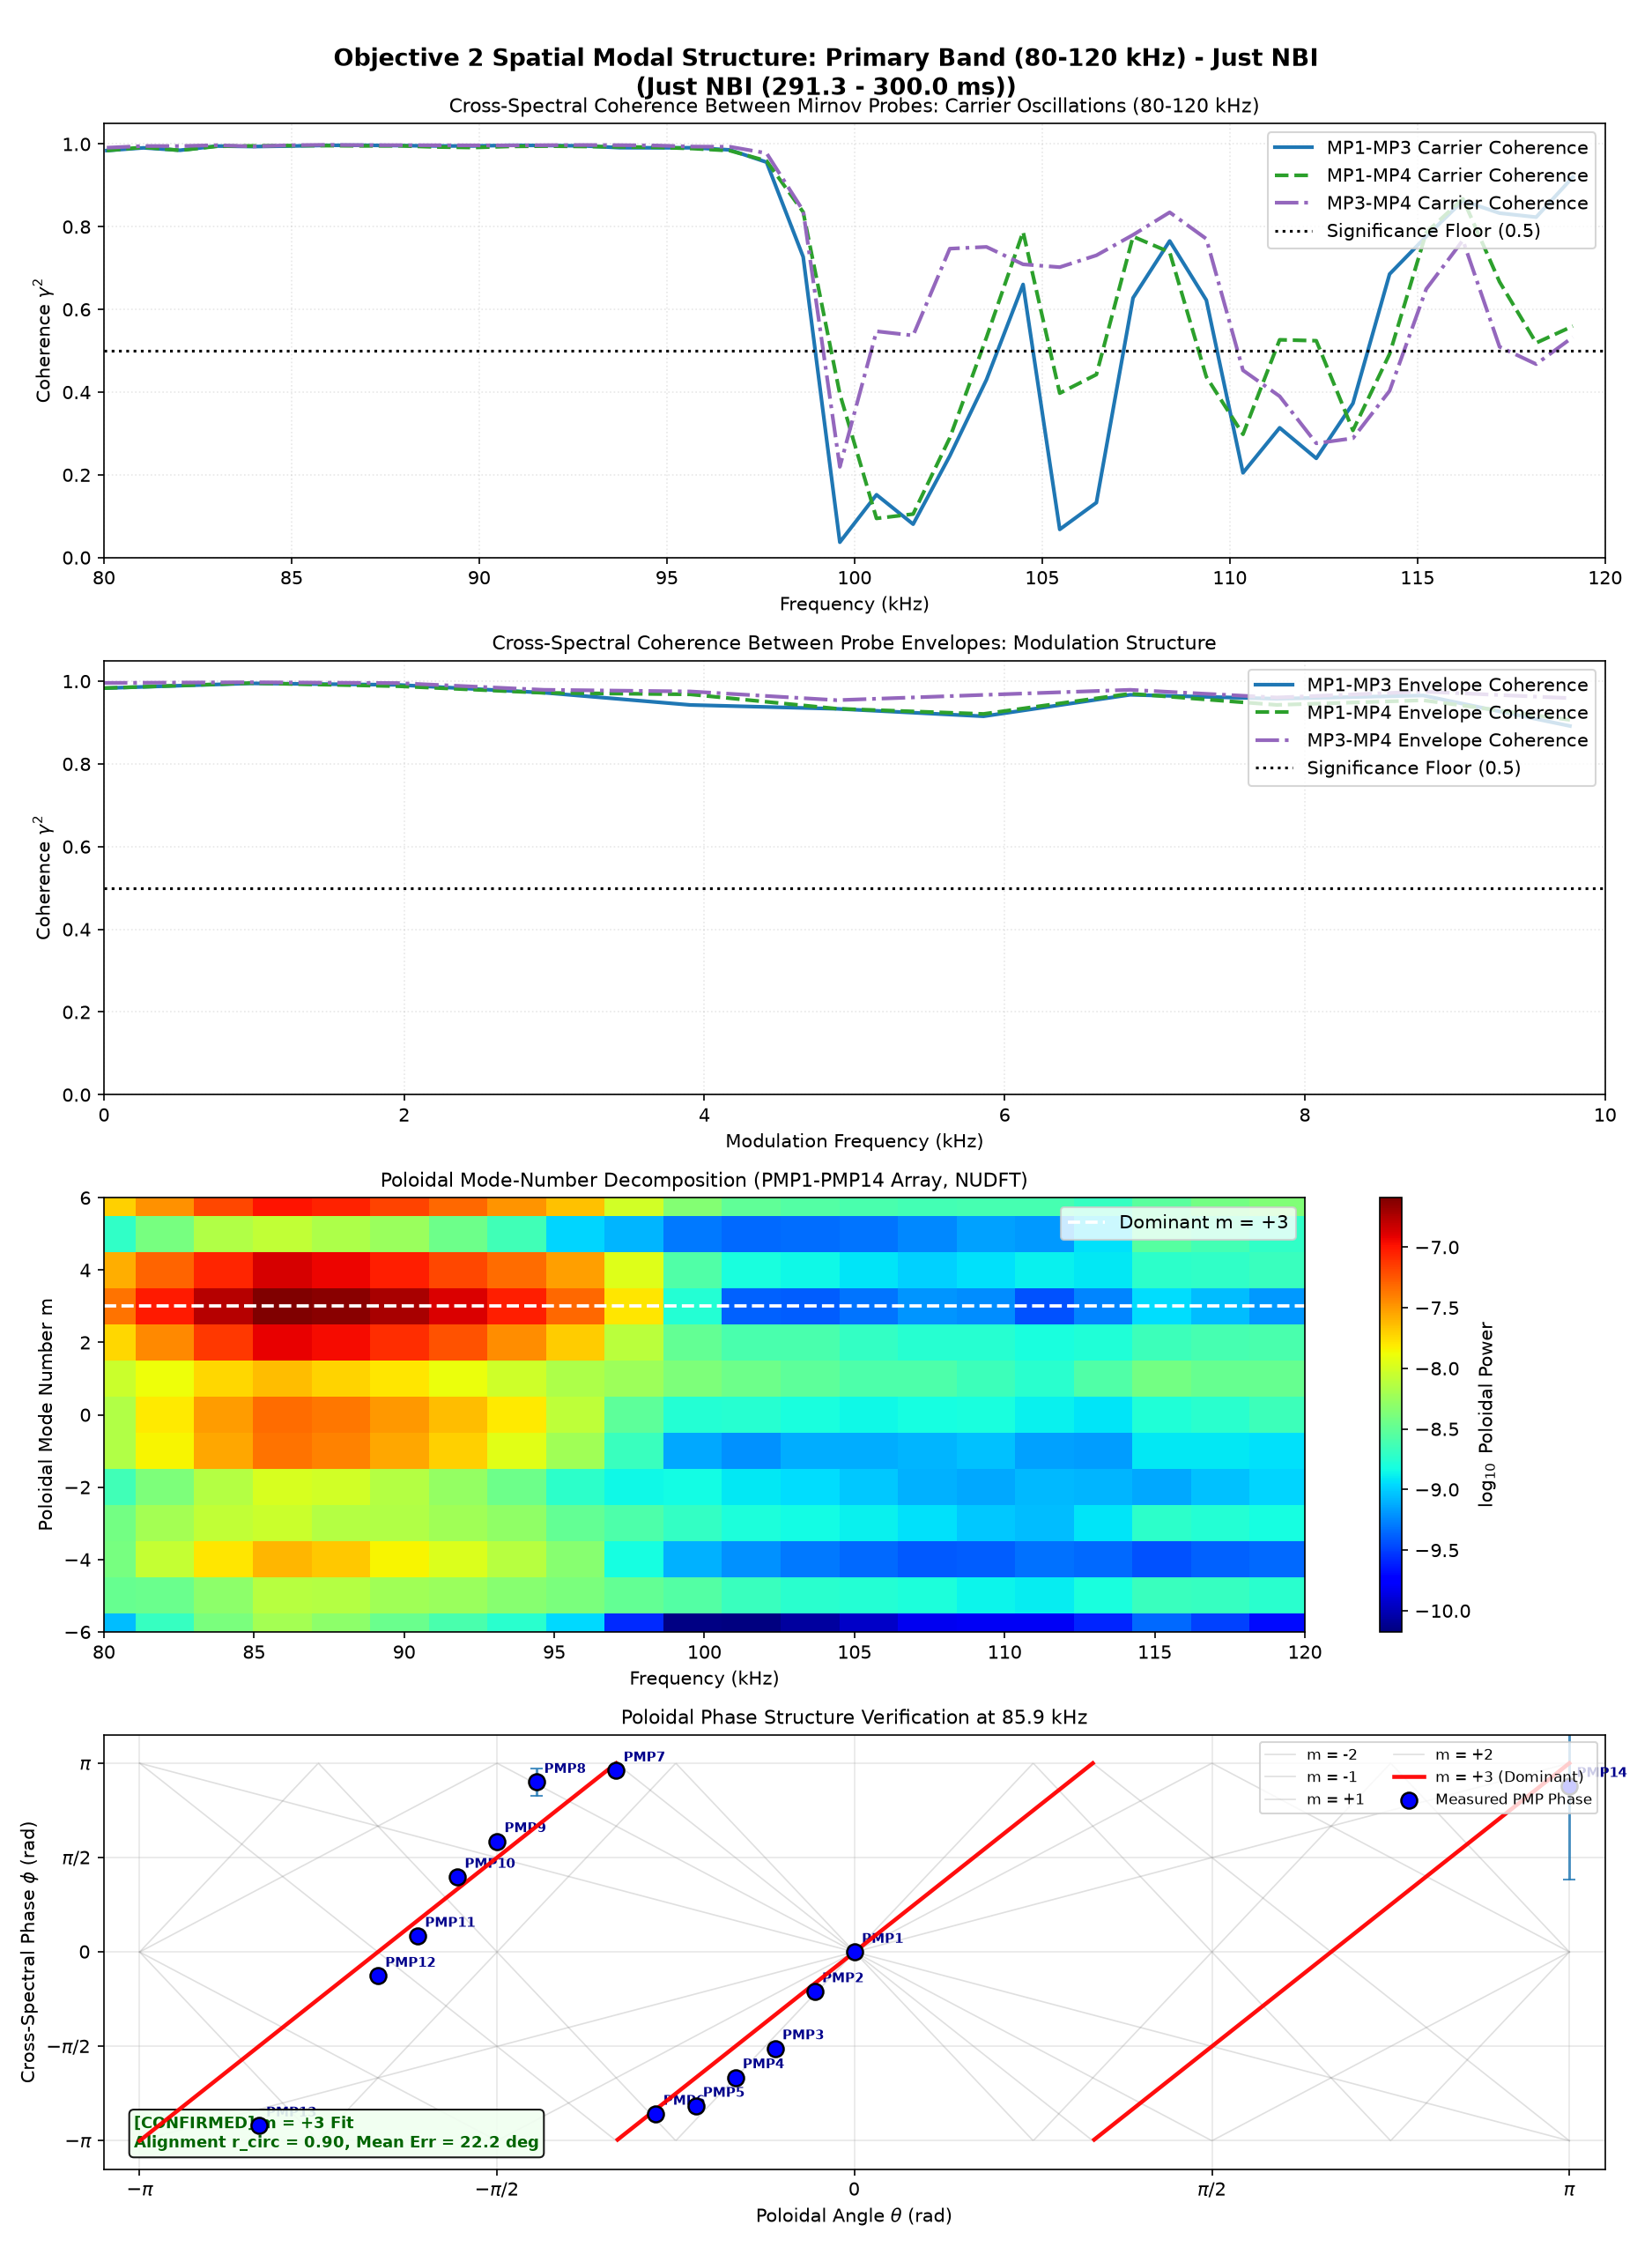
\includegraphics[width=\textwidth,height=0.66\textheight,keepaspectratio]{Images/heating_phase_comparison/mhd_analysis_objective2_structure_88653_80_120kHz_NBI_only.png}
        \end{column}
    \end{columns}
\end{frame}

\begin{frame}{Backup: Objective 2 Comparative -- Poloidal Mode Number \& Phase}
    \small
    \centering
    \begin{tabular}{llccccc}
        \toprule
        Band & Window & $m$ & $f$ (kHz) & $r_{\text{circ}}$ & Mean Err. ($^\circ$) & Status \\
        \midrule
        Secondary (40--80 kHz) & ECH+NBI  & $+6$ & 48.8 & 0.216 & 92.3 & Unconfirmed \\
        Secondary (40--80 kHz) & NBI-only & $+2$ & 41.0 & 0.632 & 81.1 & Unconfirmed \\
        Primary (80--120 kHz) & ECH+NBI  & $+3$ & 89.8 & 0.882 & 26.7 & \textbf{Confirmed} \\
        Primary (80--120 kHz) & NBI-only & $+3$ & 85.9 & 0.902 & 22.2 & \textbf{Confirmed} \\
        \bottomrule
    \end{tabular}
\end{frame}

\begin{frame}{Backup: Evolution of Mode Envelopes vs.\ Plasma Current}
    \begin{figure}[h!]
        \centering
        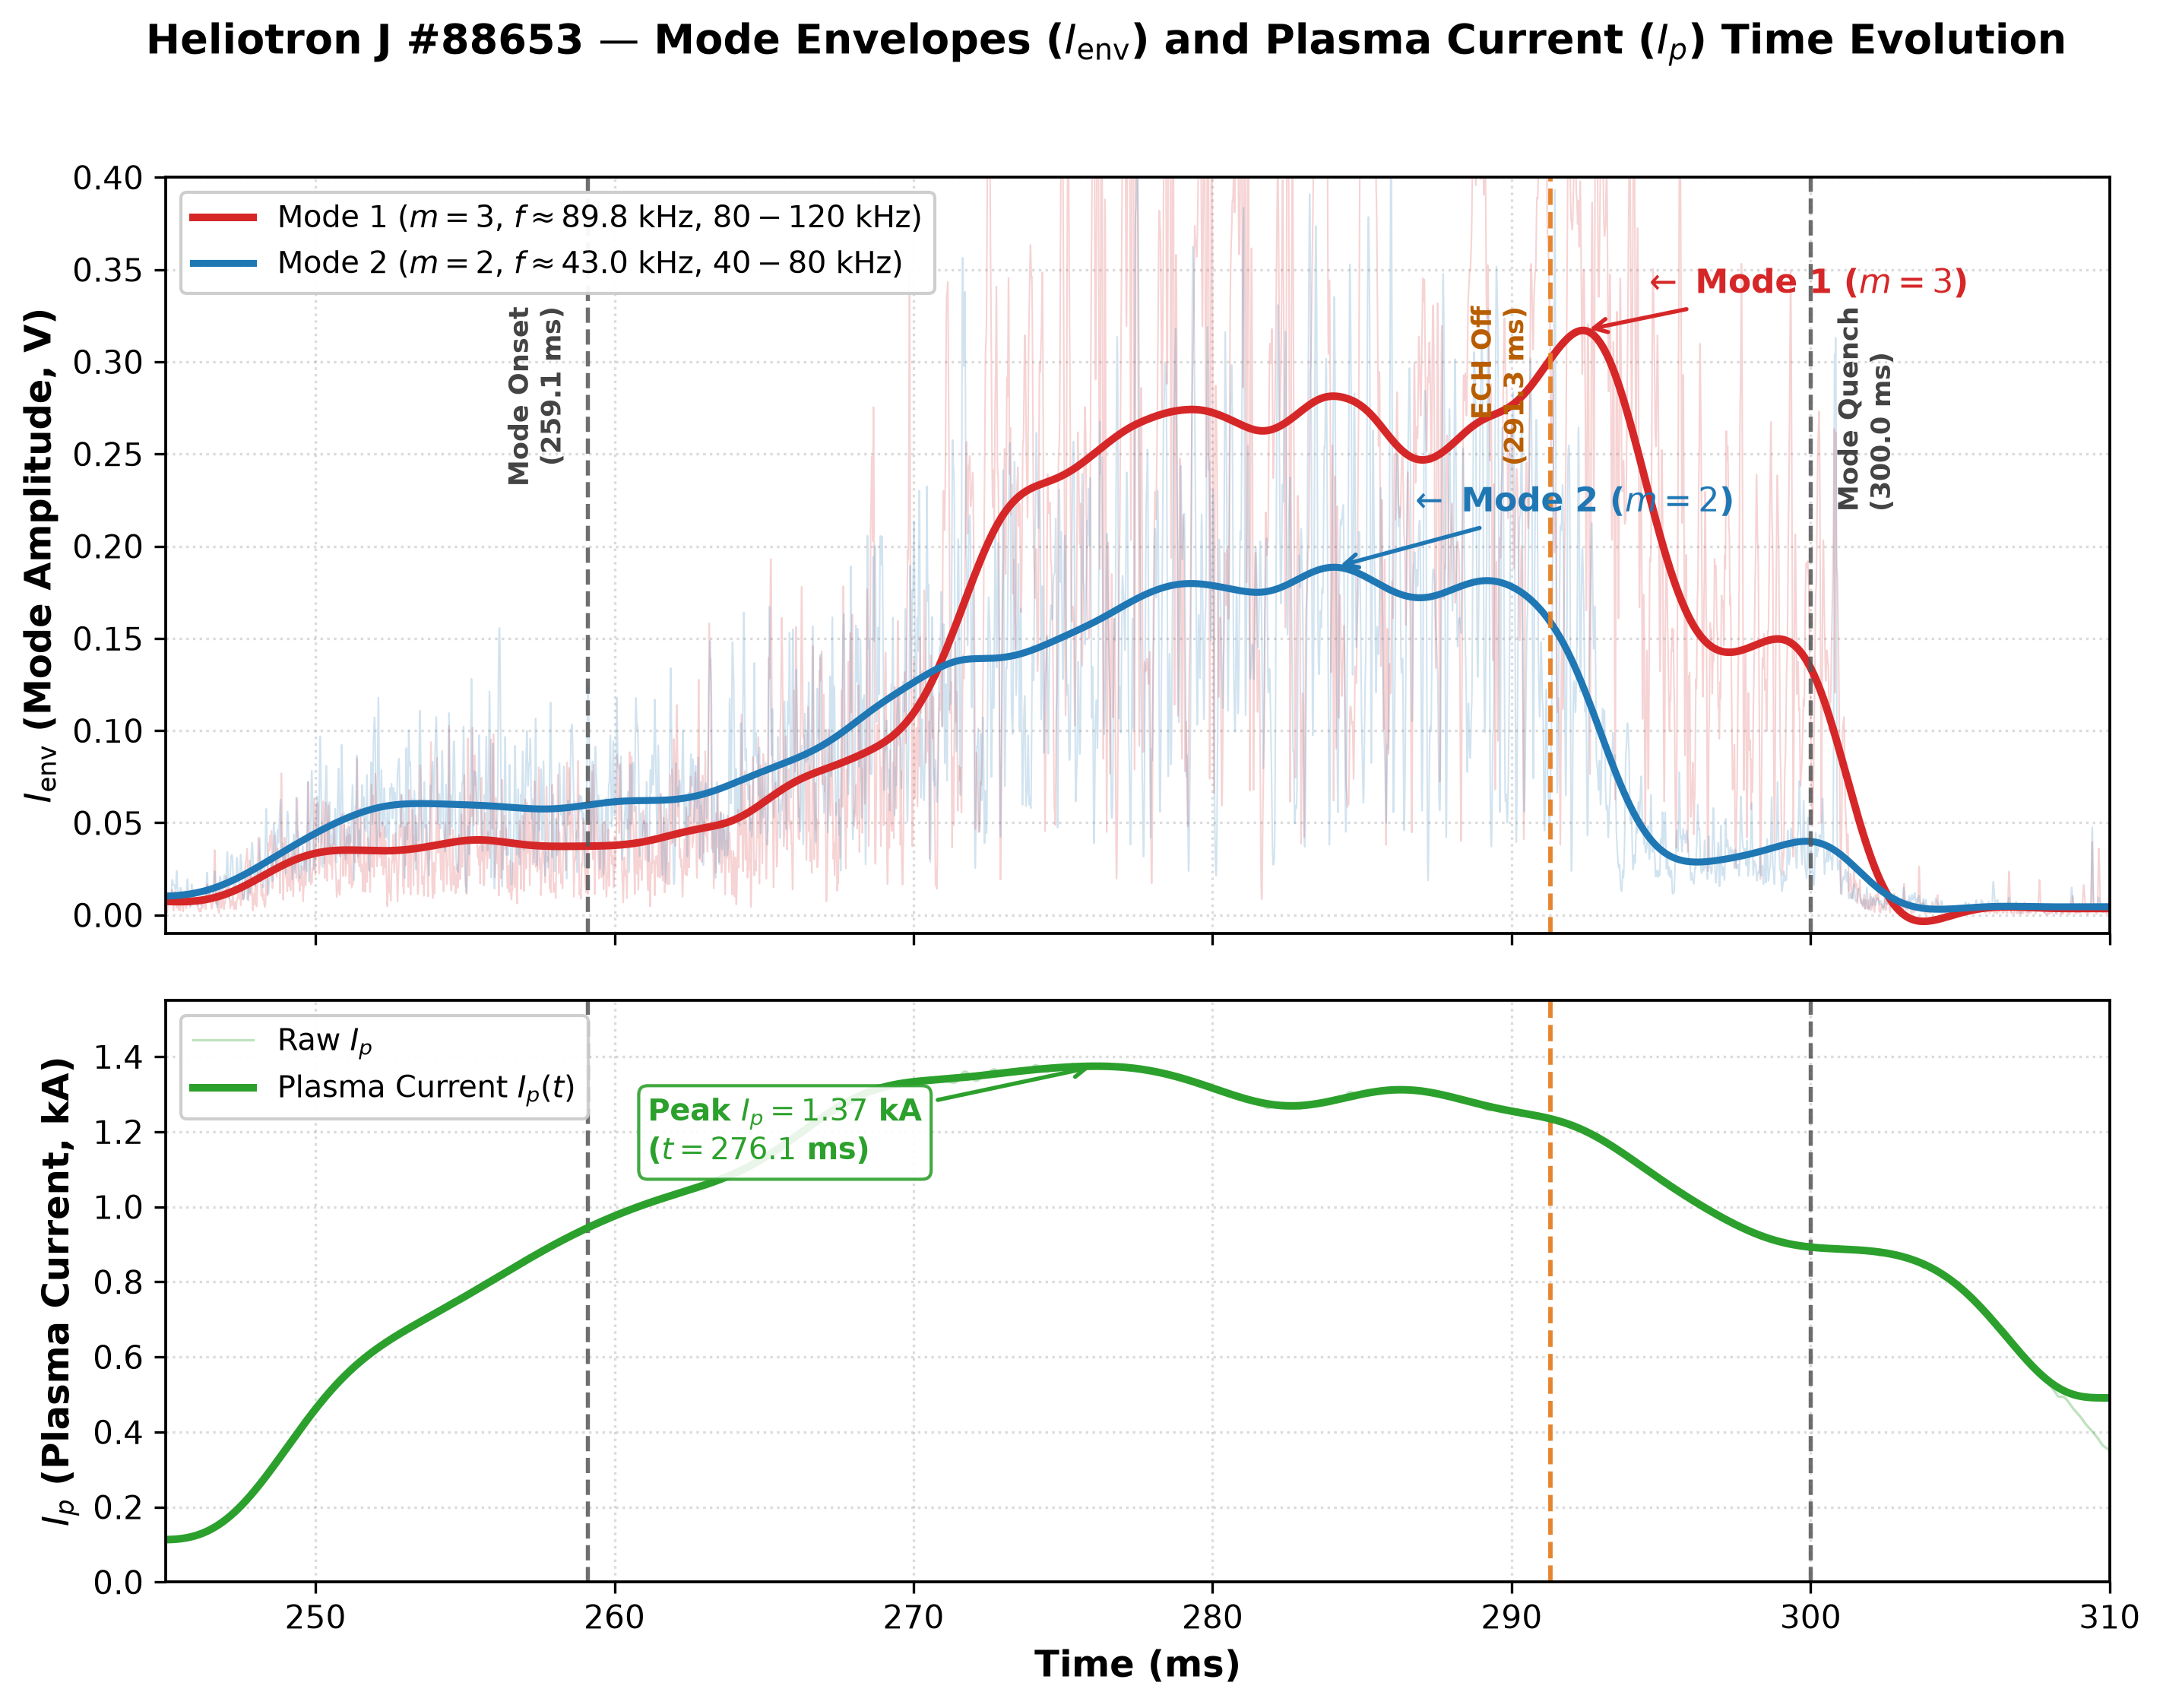
\includegraphics[height=0.75\textheight]{Images/obj2_dynamics_and_structure/mhd_mode_envelopes_and_ip_evolution_shot_88653.png}
    \end{figure}
    \tiny
    \textbf{Correction:} the ``Mode 2 quenches'' annotation on this figure is
    an artifact of the \emph{fixed} 40--80 kHz Bessel band losing the
    secondary mode as it downshifts to 35--40 kHz after ECH shut-off. An
    adaptive-band re-extraction (25--65 kHz) shows the envelope at
    $4.6\times$ the local noise floor at $t=295$--298 ms -- the mode
    downshifts, it does \emph{not} vanish. (Mode~2's $m=2$ is tentative, see the
    poloidal-number table.)
\end{frame}

\begin{frame}{Backup: Hysteresis Loop -- Plasma Current vs.\ Mode Envelope}
    \begin{figure}[h!]
        \centering
        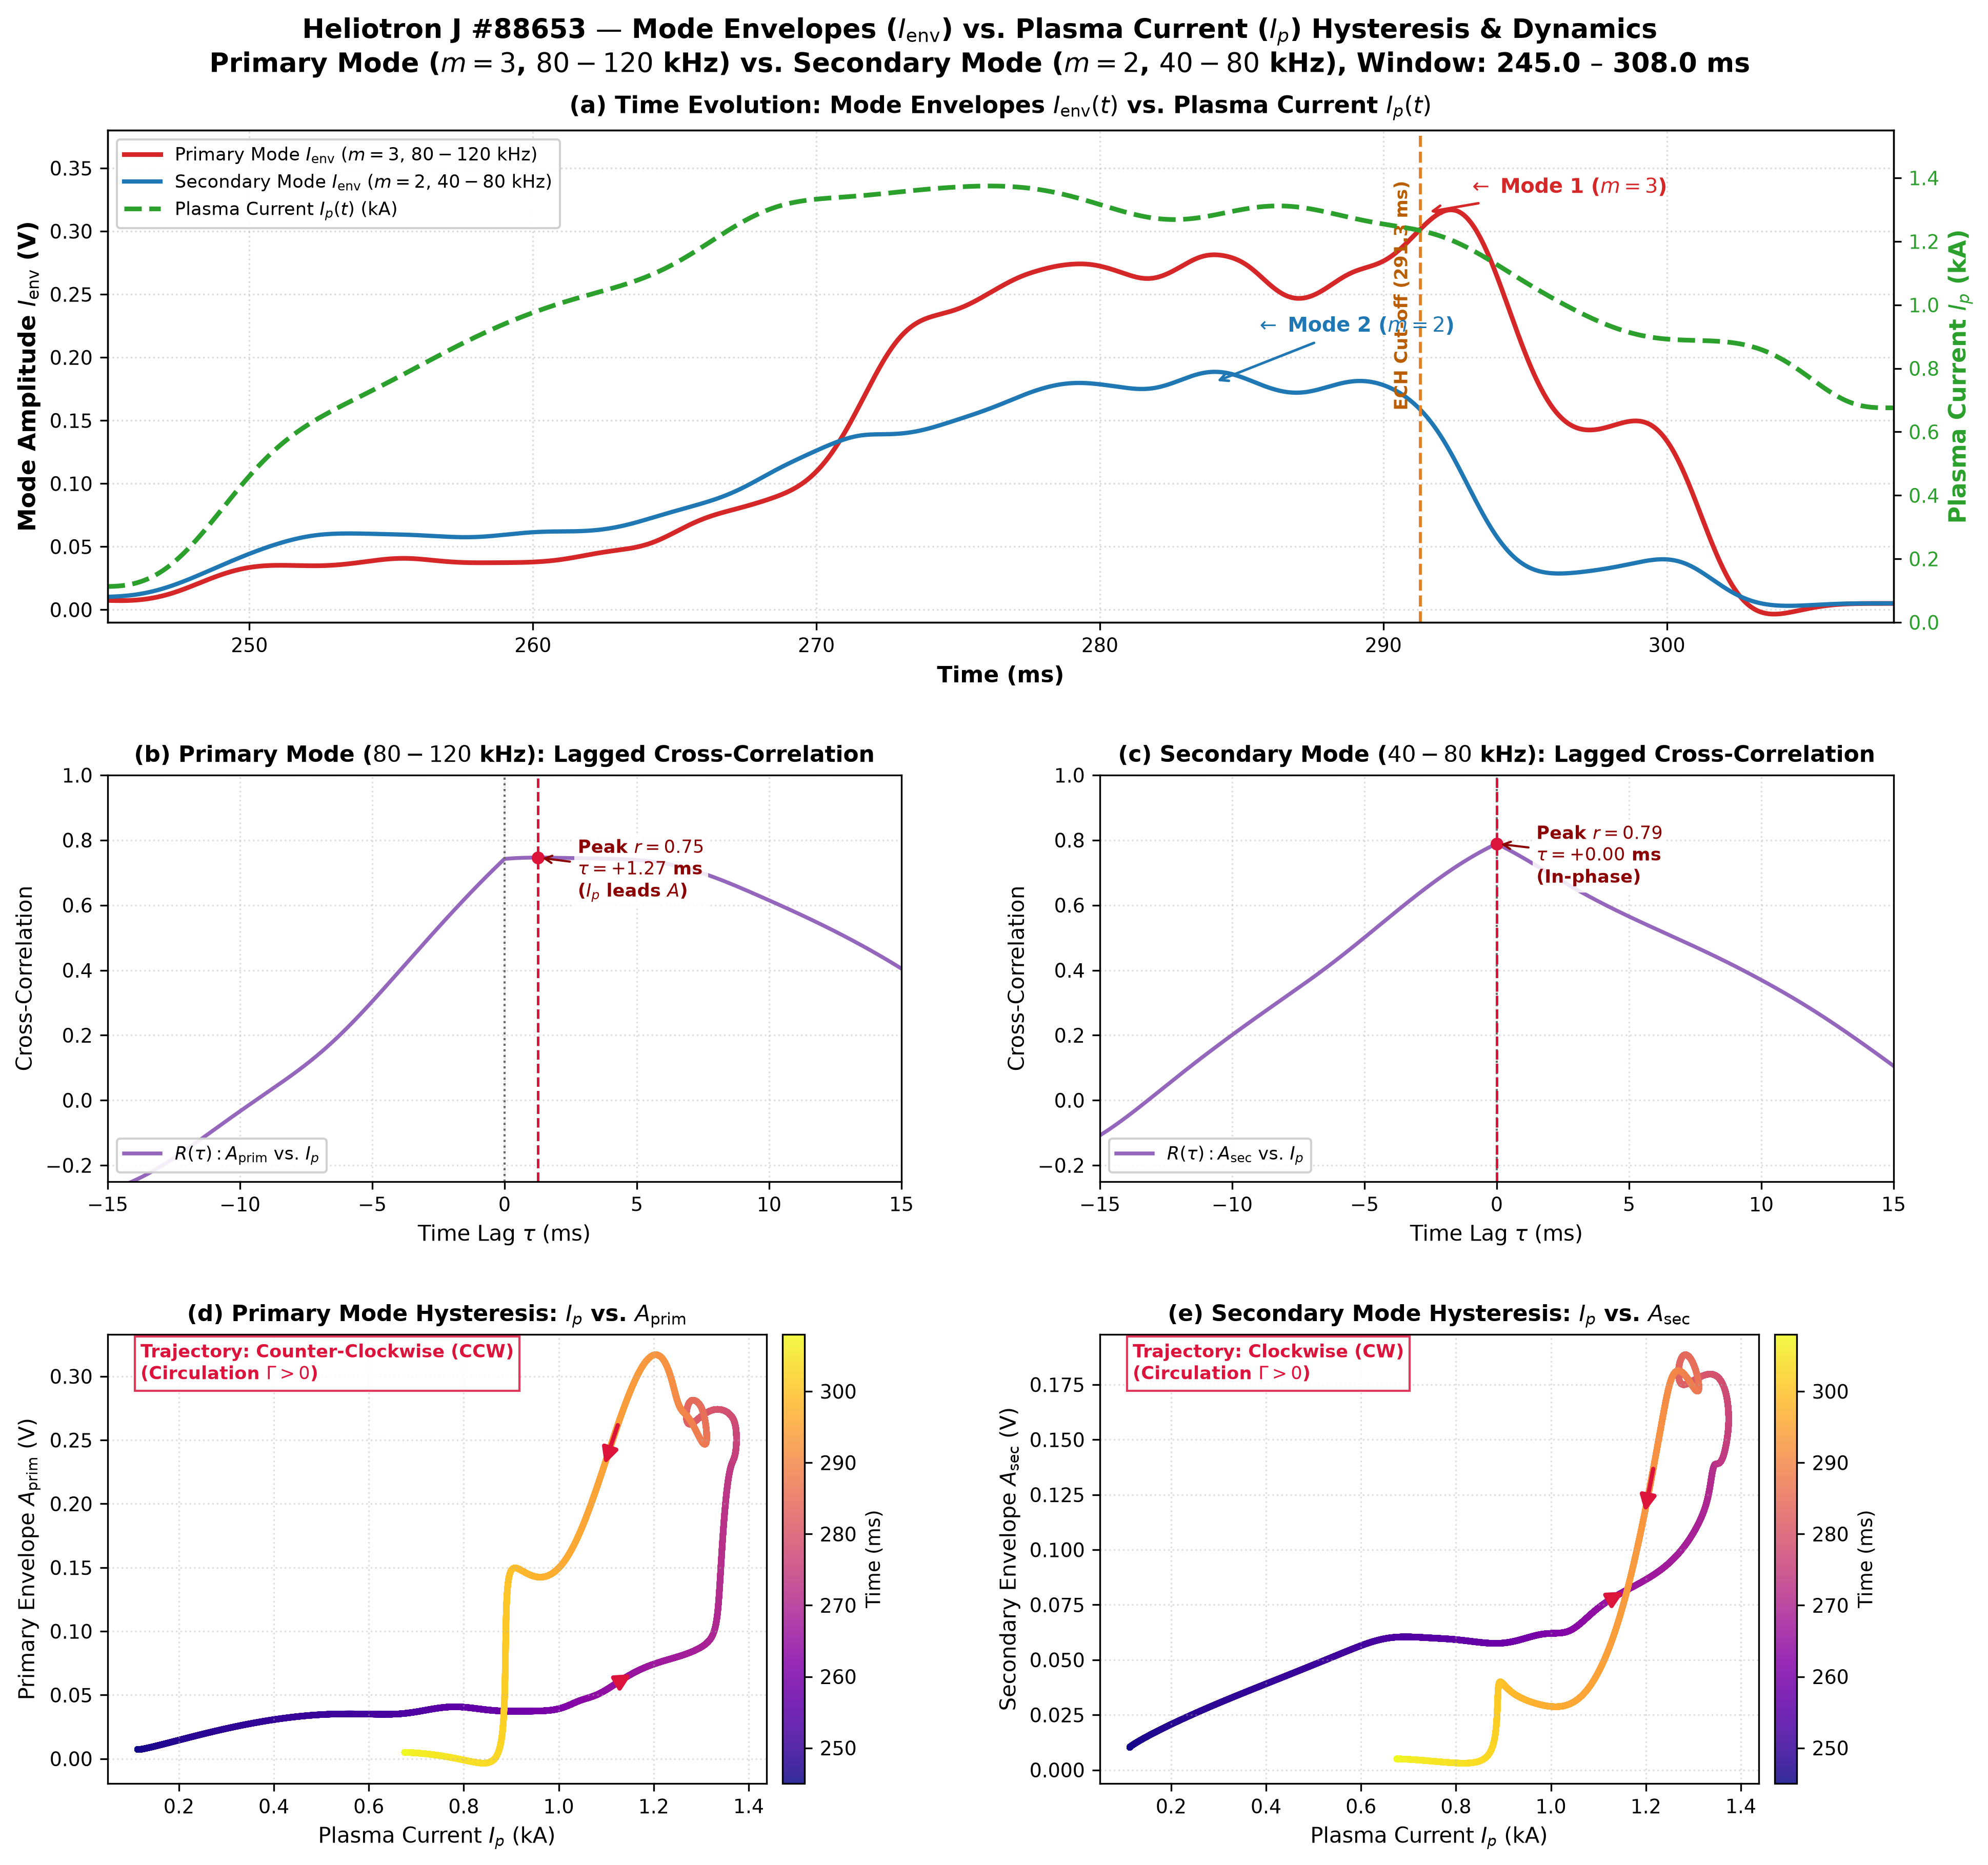
\includegraphics[height=0.75\textheight]{Images/obj2_dynamics_and_structure/mhd_hysteresis_ip_vs_envelope_dual_modes_shot_88653.png}
    \end{figure}
    \tiny
    \textbf{Same correction applies:} the apparent secondary-mode collapse
    in this hysteresis trace reflects the same fixed-band filter-edge
    effect, not a physical quench -- see the previous backup slide.
\end{frame}

\begin{frame}{Backup: Dual-Mode Envelope Coherence (Inter-Mode Modulation)}
    \begin{figure}[h!]
        \centering
        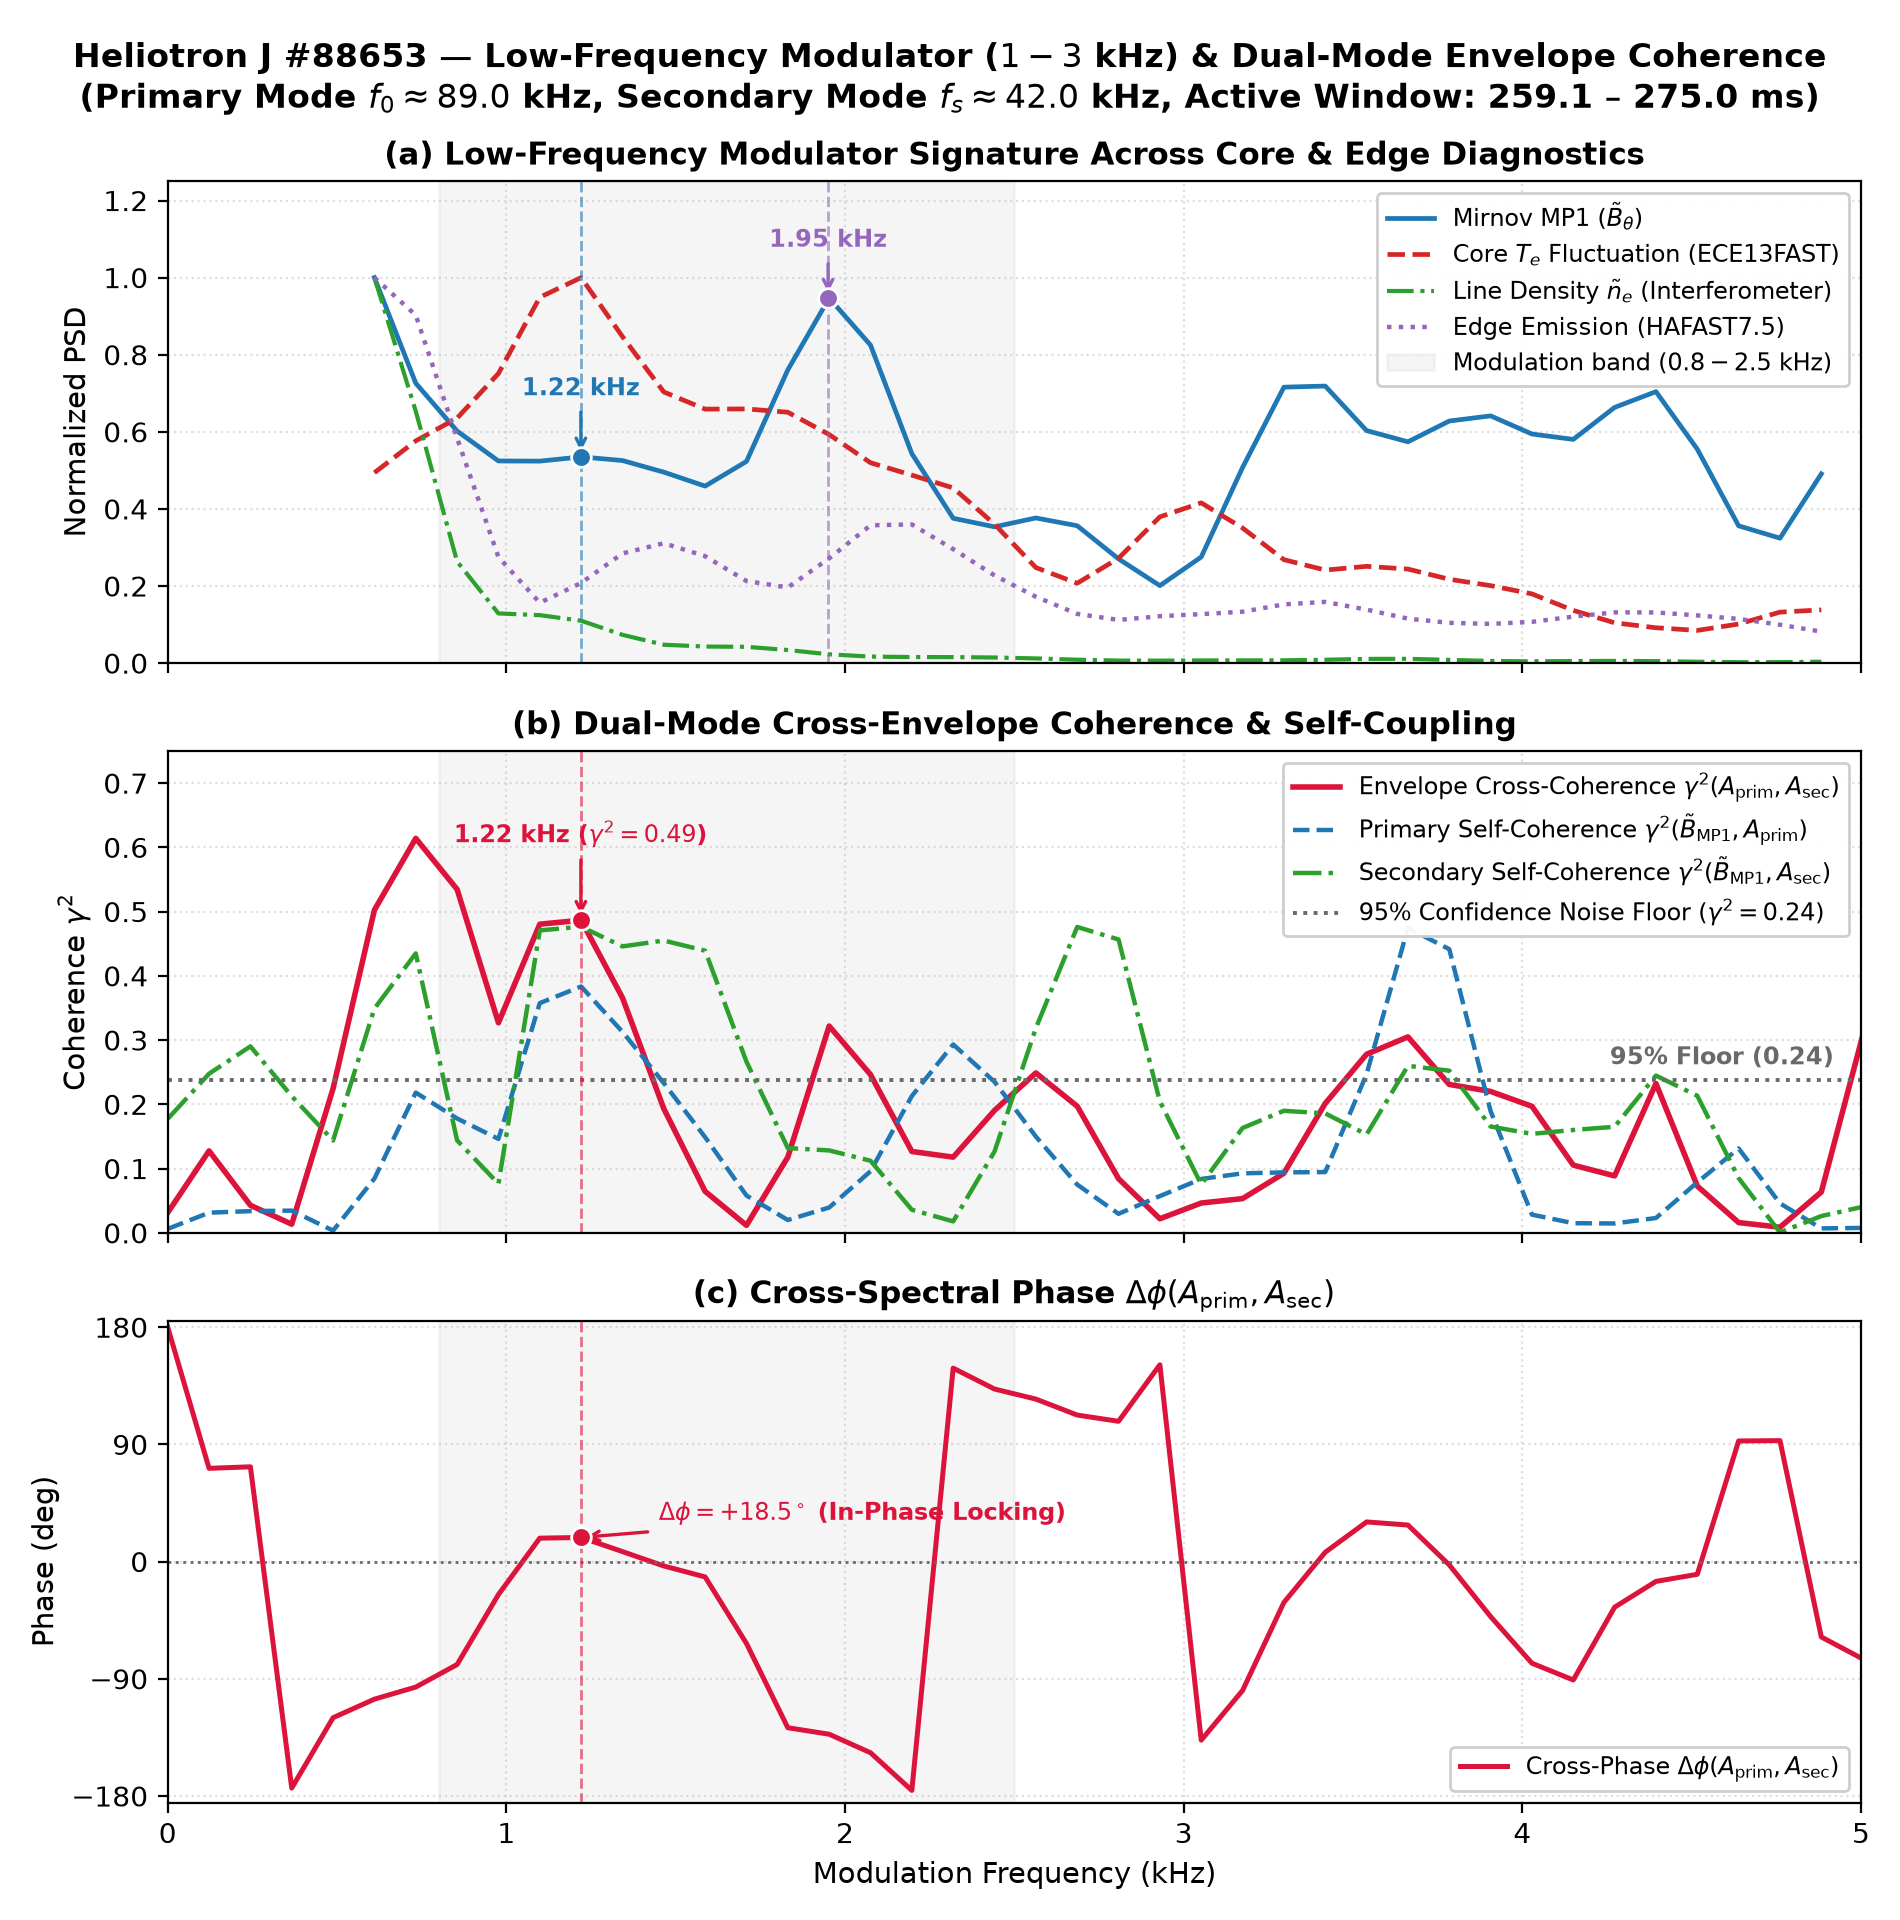
\includegraphics[height=0.85\textheight]{Images/obj2_dynamics_and_structure/mhd_modulator_dual_mode_coherence_shot_88653.png}
    \end{figure}
\end{frame}

\begin{frame}{Backup: Secondary--Primary Mode-Mixing Correlation}
    \begin{columns}[T]
        \begin{column}{0.5\textwidth}
            \centering Secondary branch ($\sim$\SI{43}{kHz})\\
            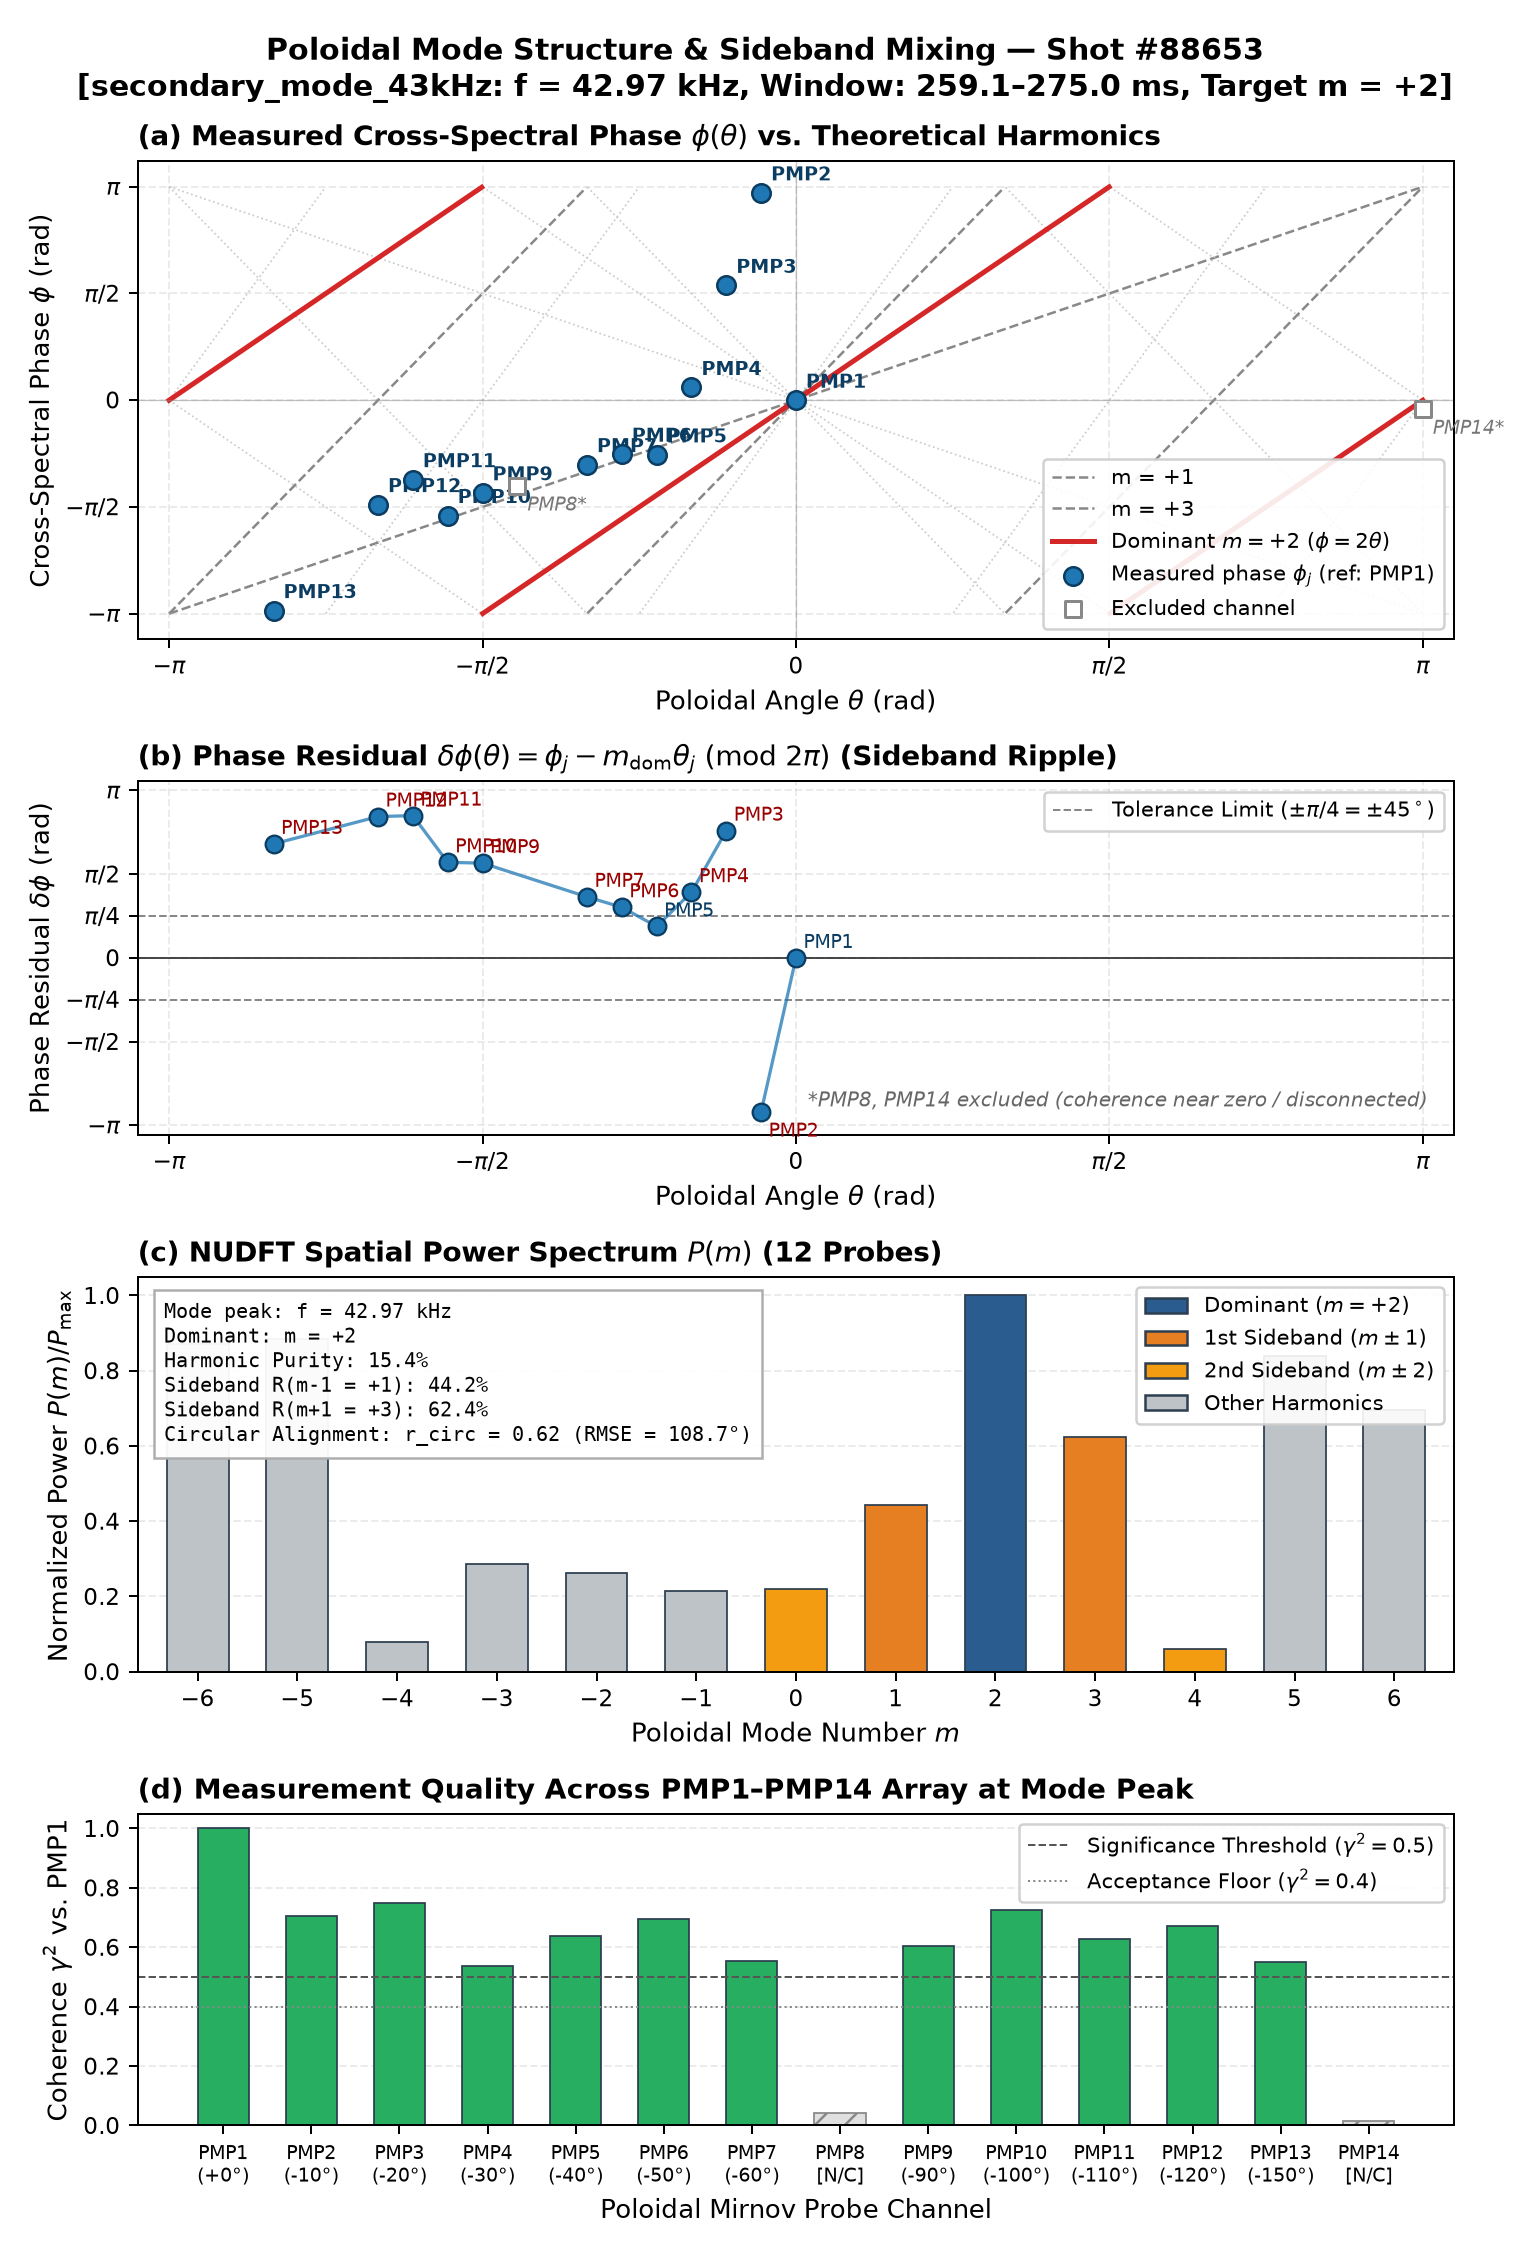
\includegraphics[width=0.62\textwidth]{Images/obj3_nonlinear_coupling/mhd_mode_mixing_shot_88653_secondary_mode_43kHz.png}
        \end{column}
        \begin{column}{0.5\textwidth}
            \centering Primary branch ($\sim$\SI{90}{kHz})\\
            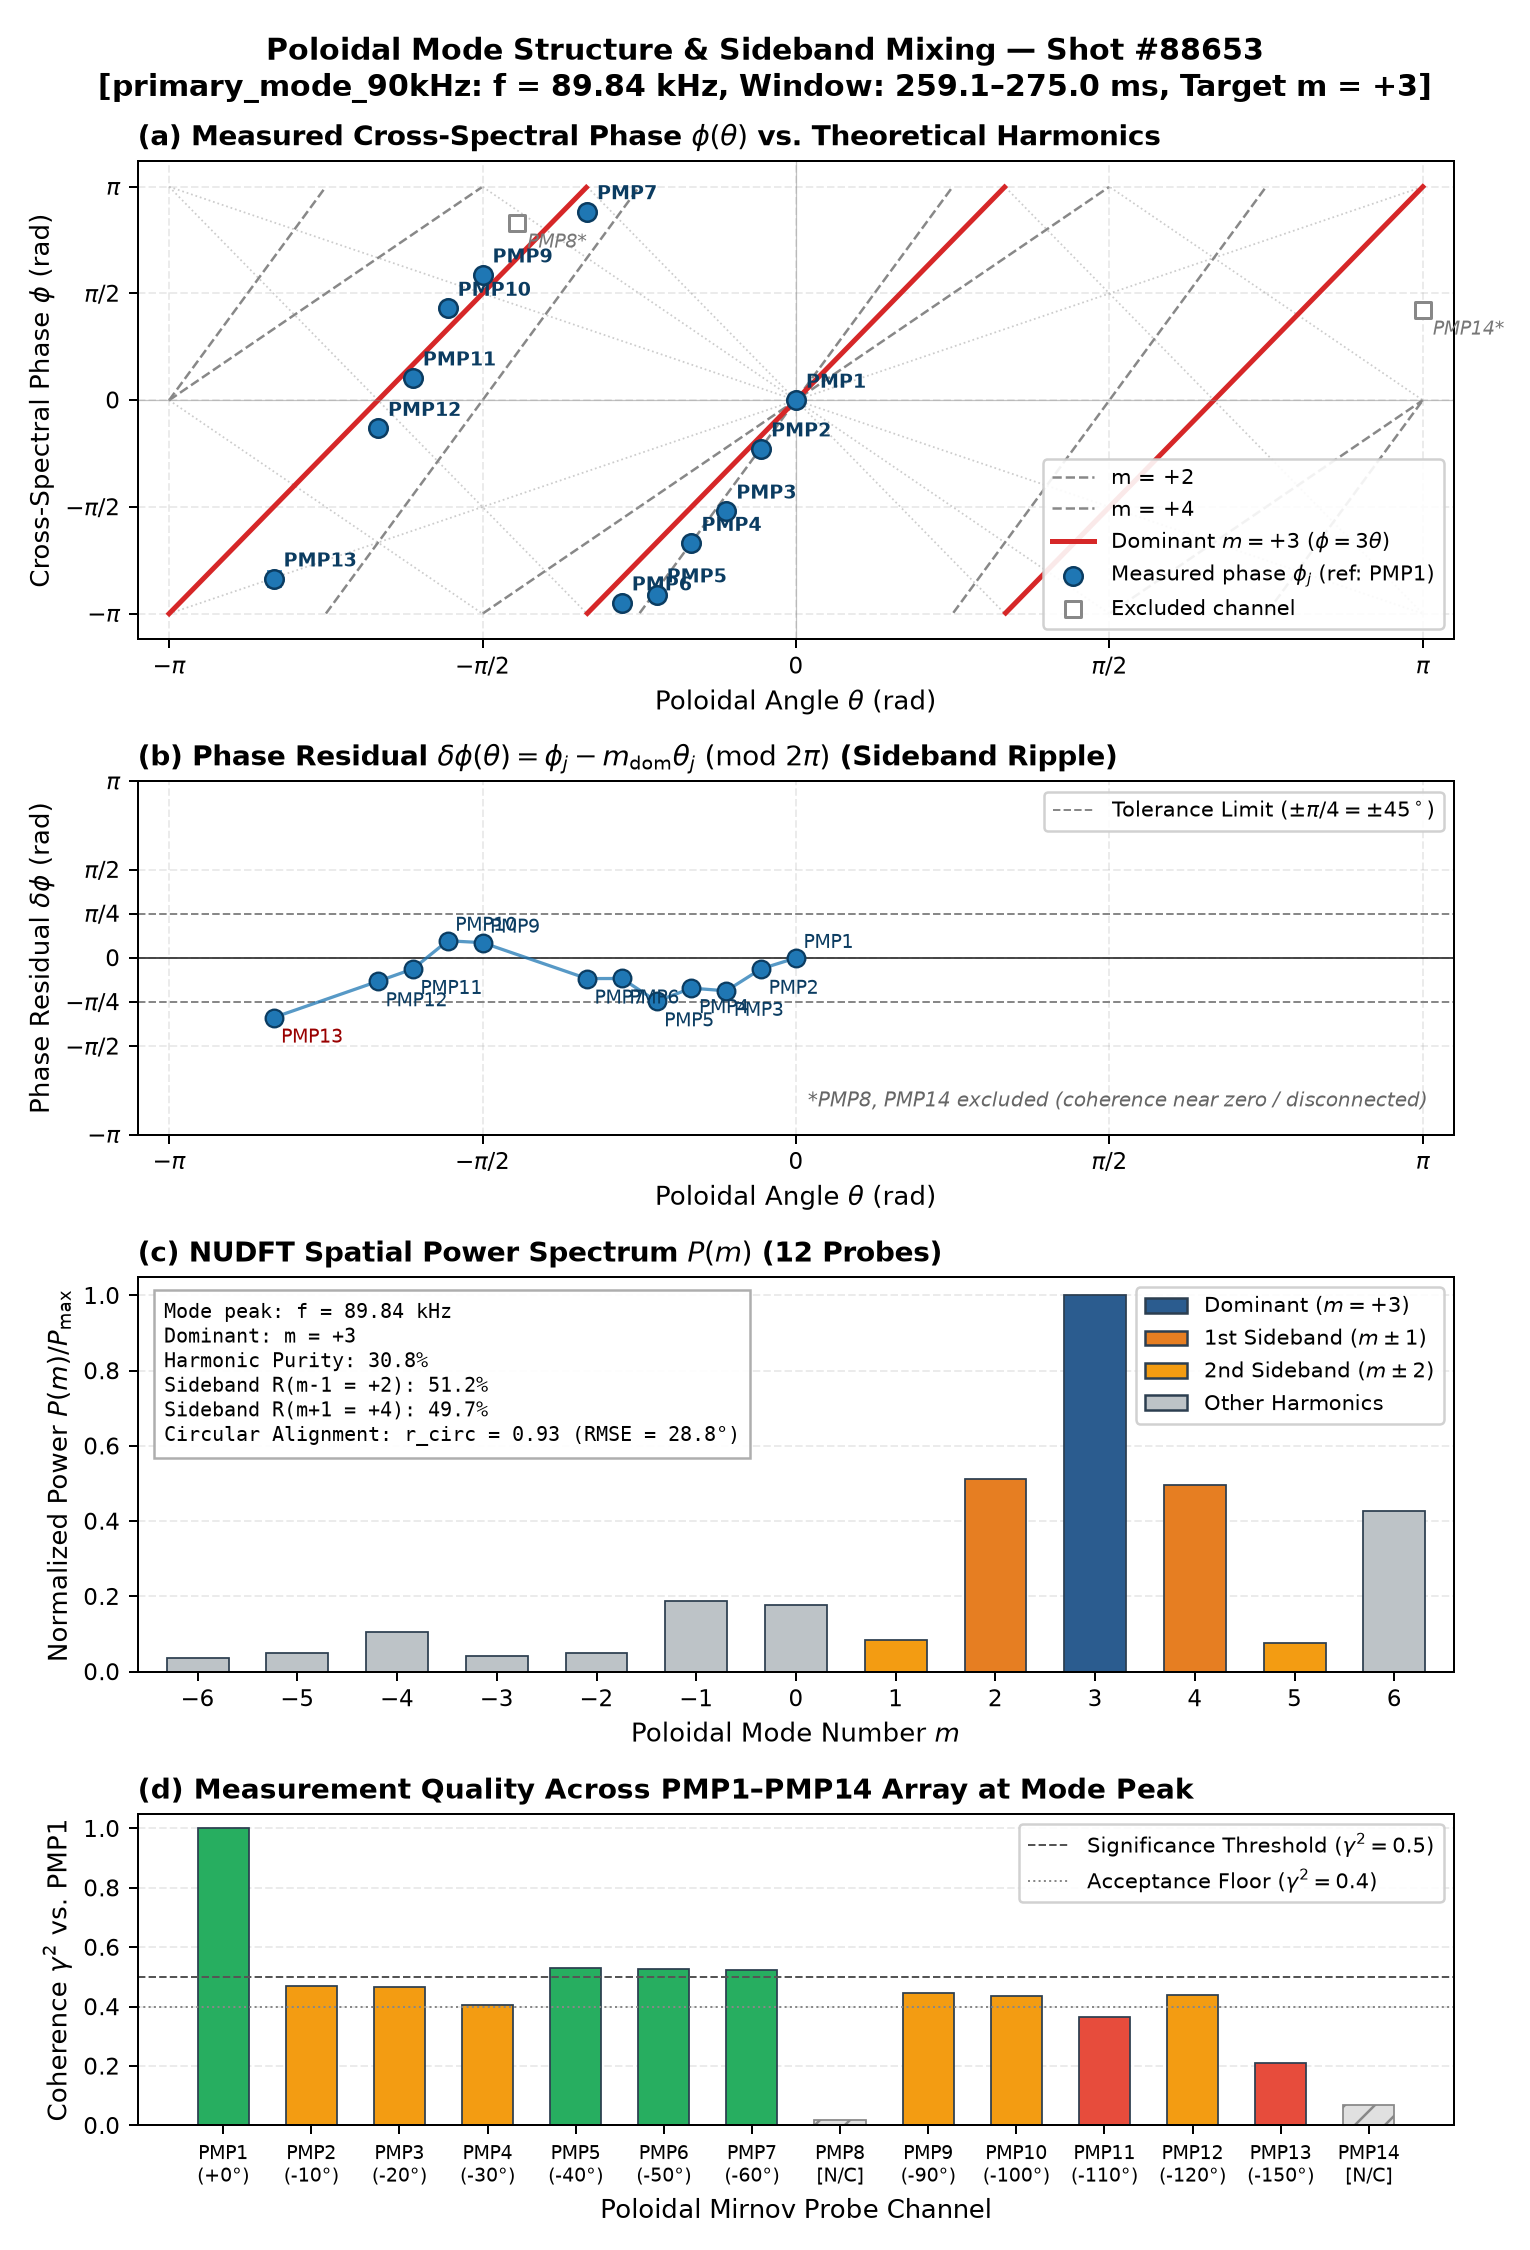
\includegraphics[width=0.62\textwidth]{Images/obj3_nonlinear_coupling/mhd_mode_mixing_shot_88653_primary_mode_90kHz.png}
        \end{column}
    \end{columns}
    \vspace{0.2cm}
    \tiny Additional correlation-metric view of inter-band mixing between the Secondary and Primary
    envelopes, complementing the dual-mode coherence above. Numbers on this slide have not
    been independently re-verified against the pipeline outputs in this round -- check
    against the underlying script before quoting specific values live.
\end{frame}

\begin{frame}{Backup: Carrier ($\tilde{B}$) vs.\ Envelope}
    \begin{figure}[h!]
        \centering
        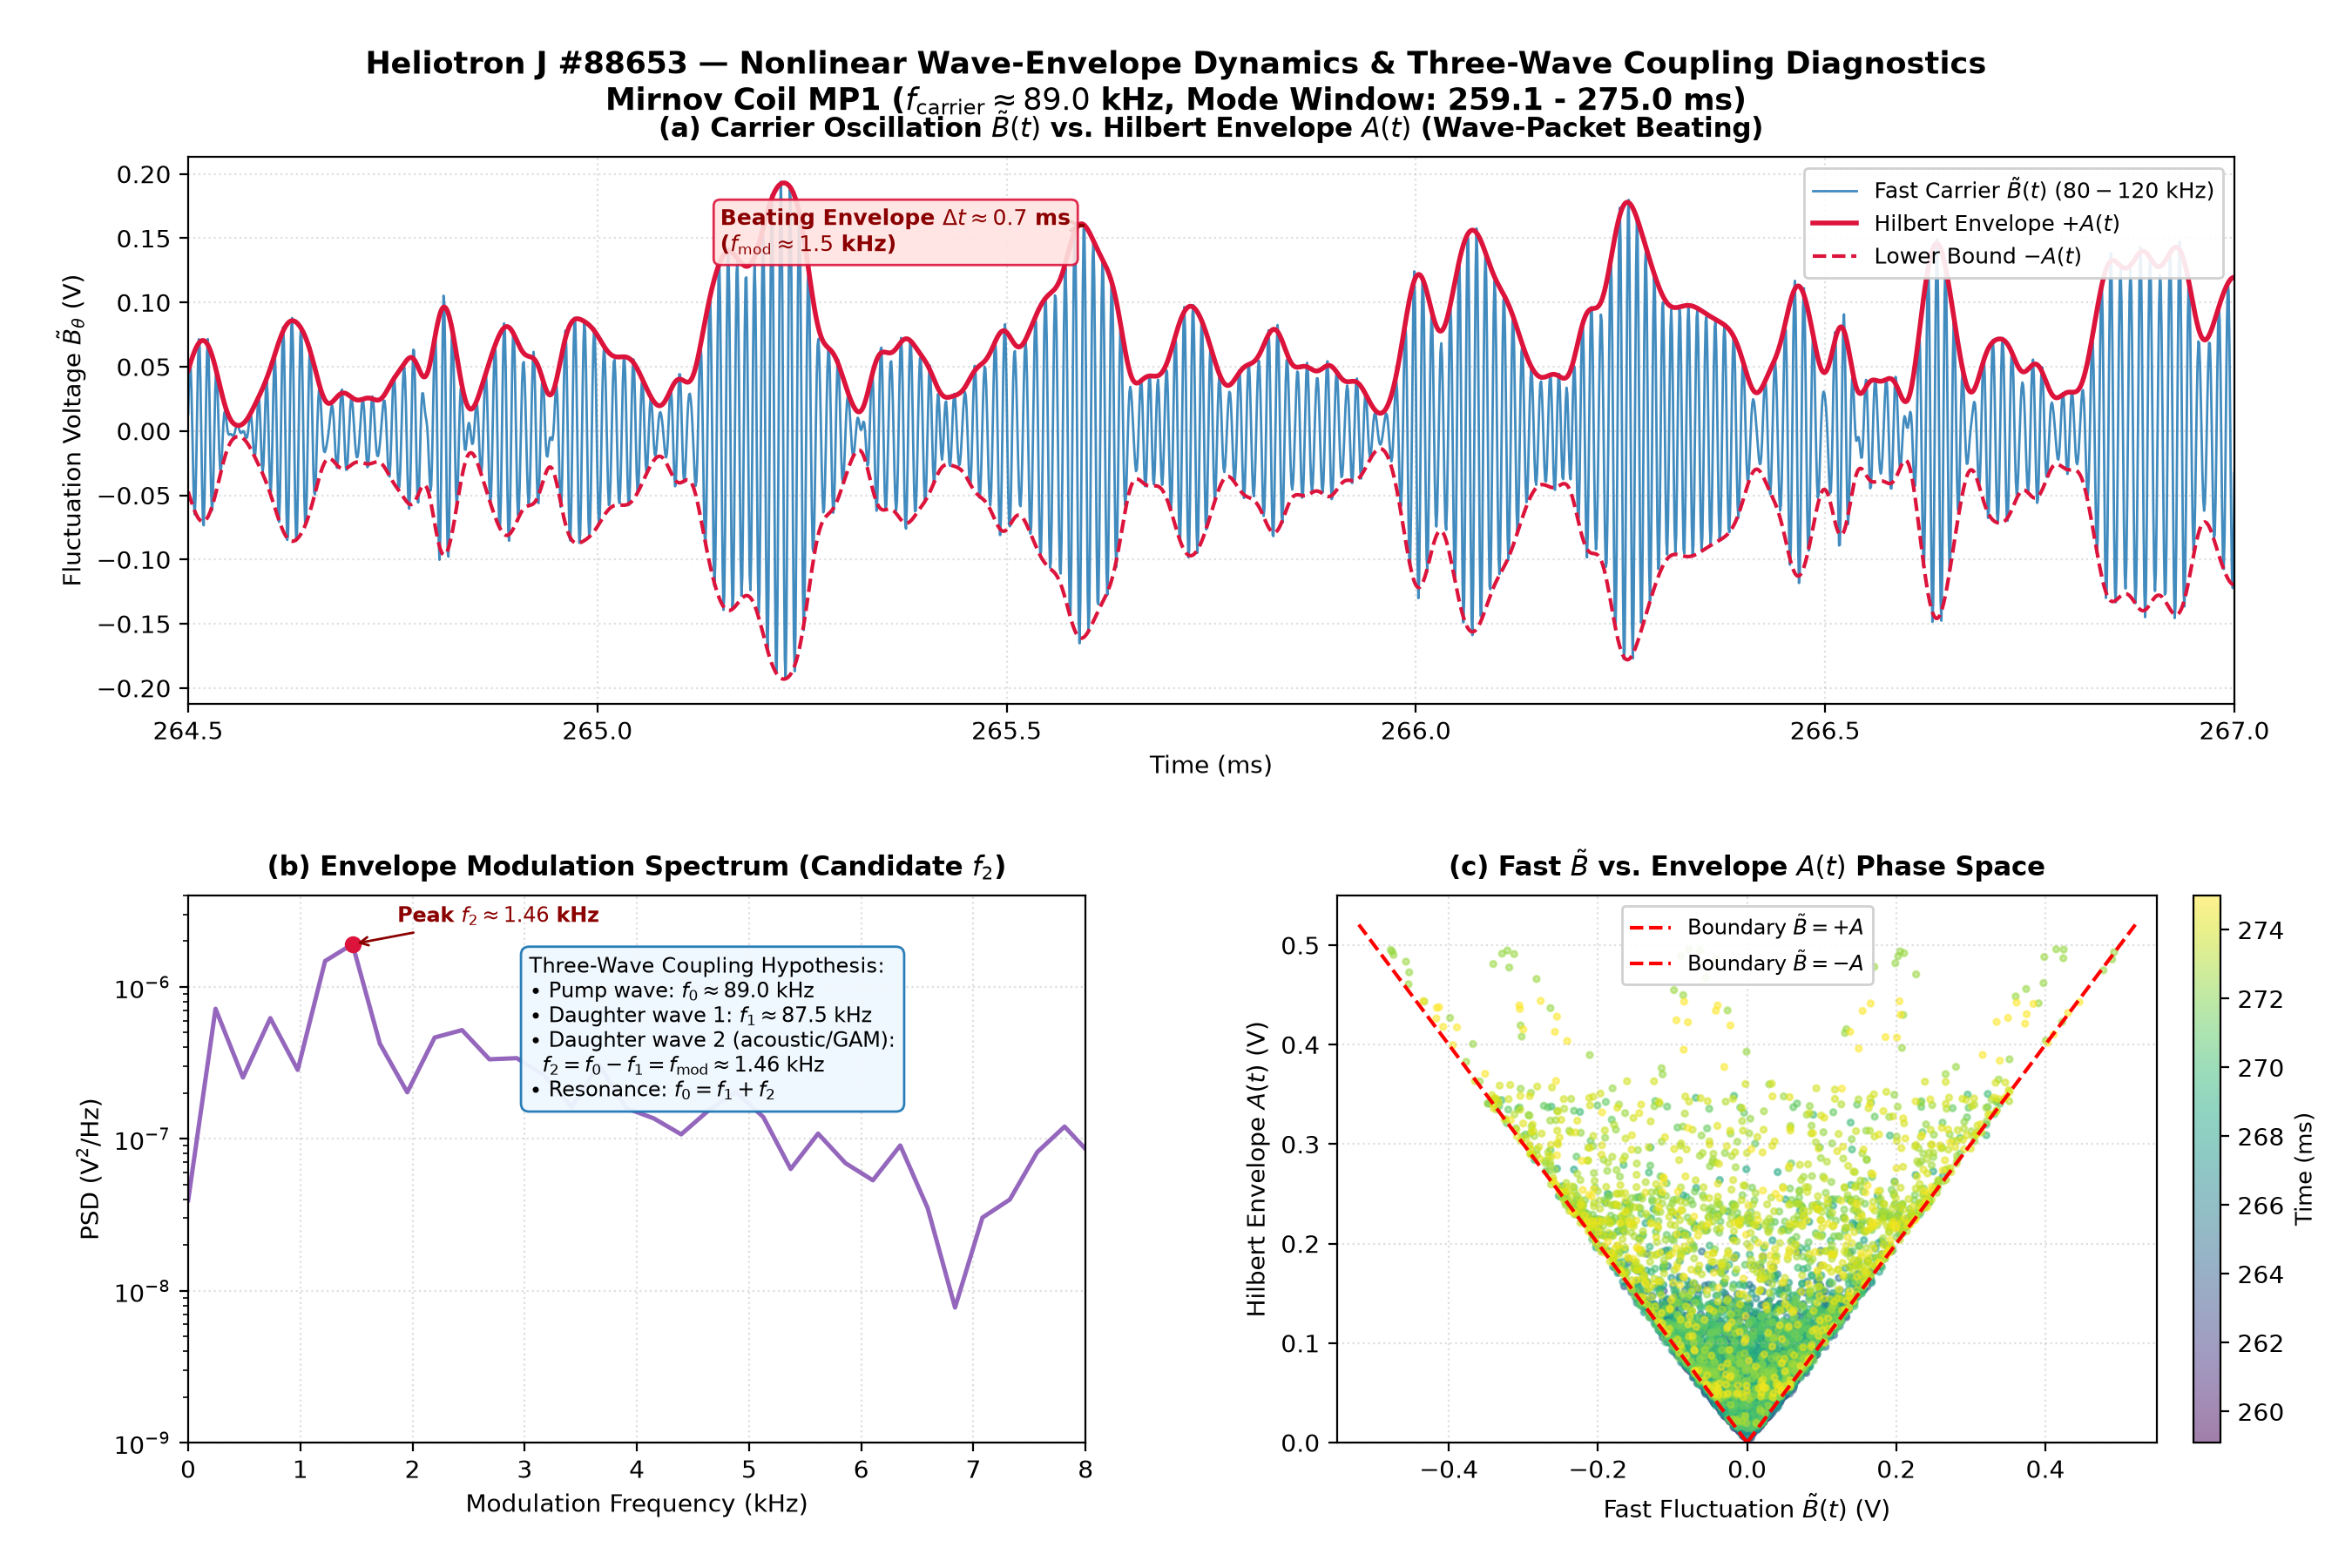
\includegraphics[height=0.85\textheight]{Images/obj2_dynamics_and_structure/mhd_b_tilde_vs_envelope_shot_88653.png}
    \end{figure}
\end{frame}

\begin{frame}{Backup: SNR vs.\ H$\alpha$ Emission Correlation}
    \begin{figure}[h!]
        \centering
        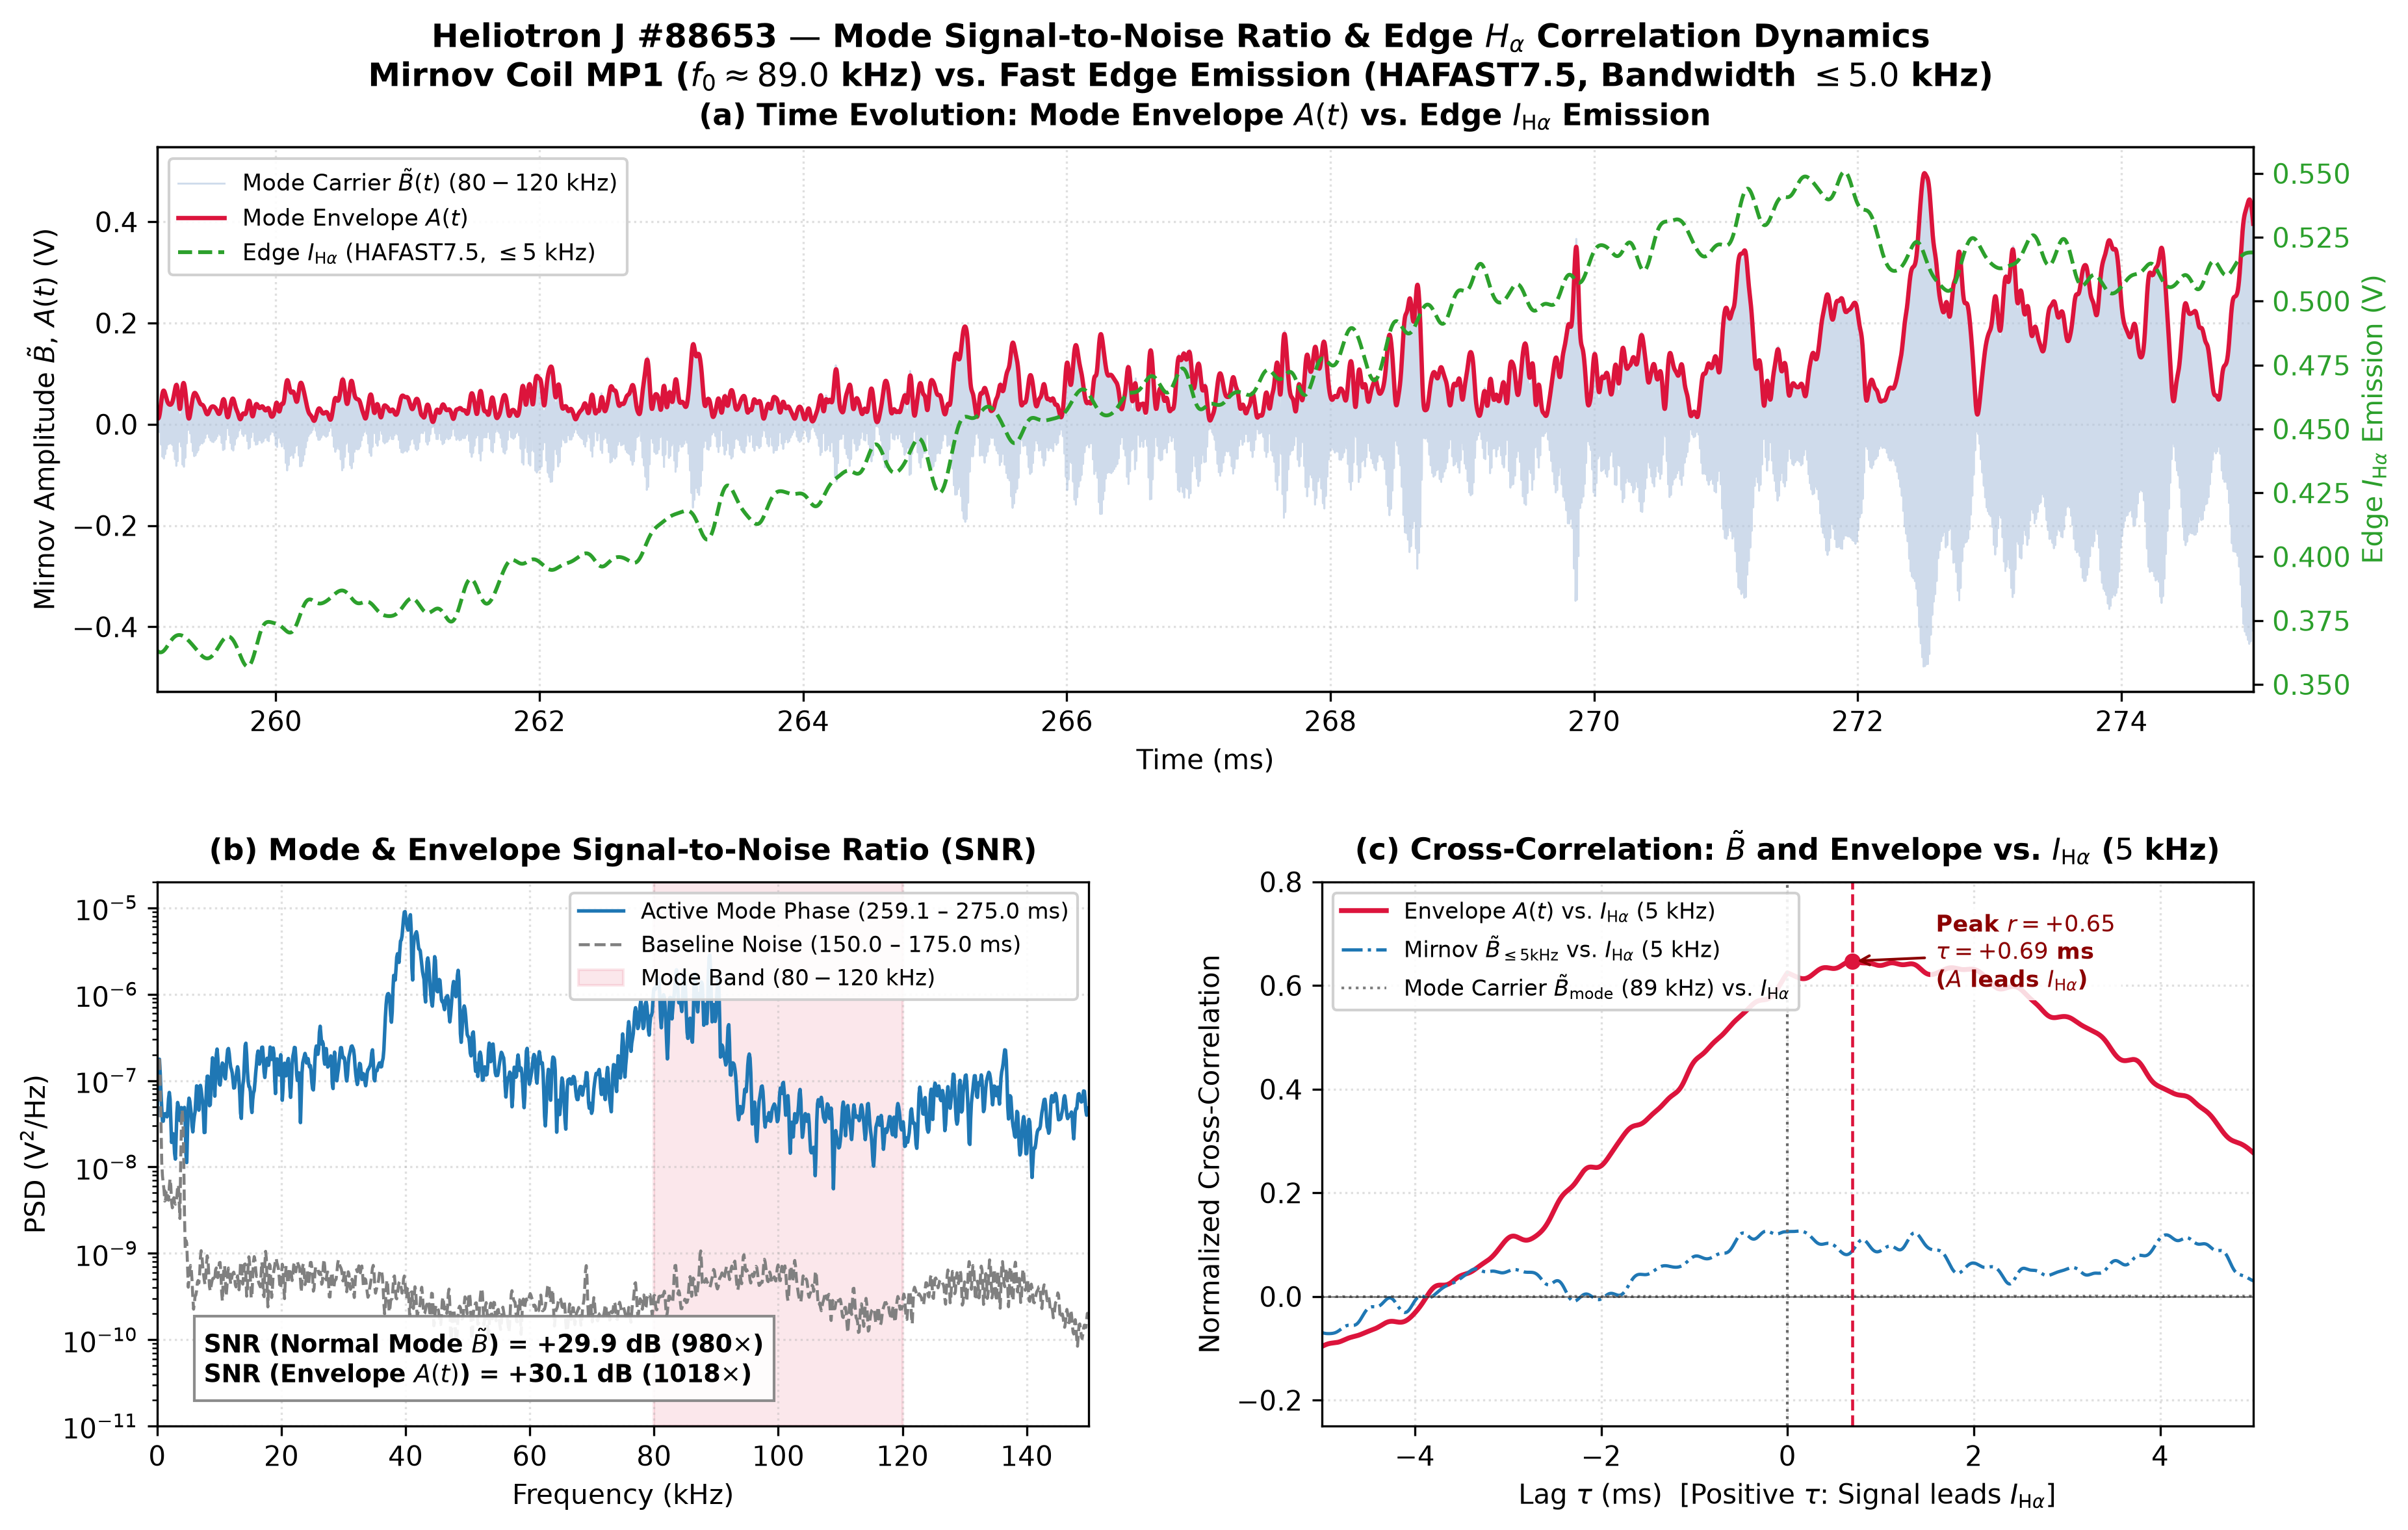
\includegraphics[height=0.85\textheight]{Images/obj2_dynamics_and_structure/mhd_snr_halpha_correlation_shot_88653.png}
    \end{figure}
\end{frame}

\subsection{Backup: Objective 3}








\begin{frame}{Backup: Objective 3 -- Burst Window Detection}
    \begin{figure}[h!]
        \centering
        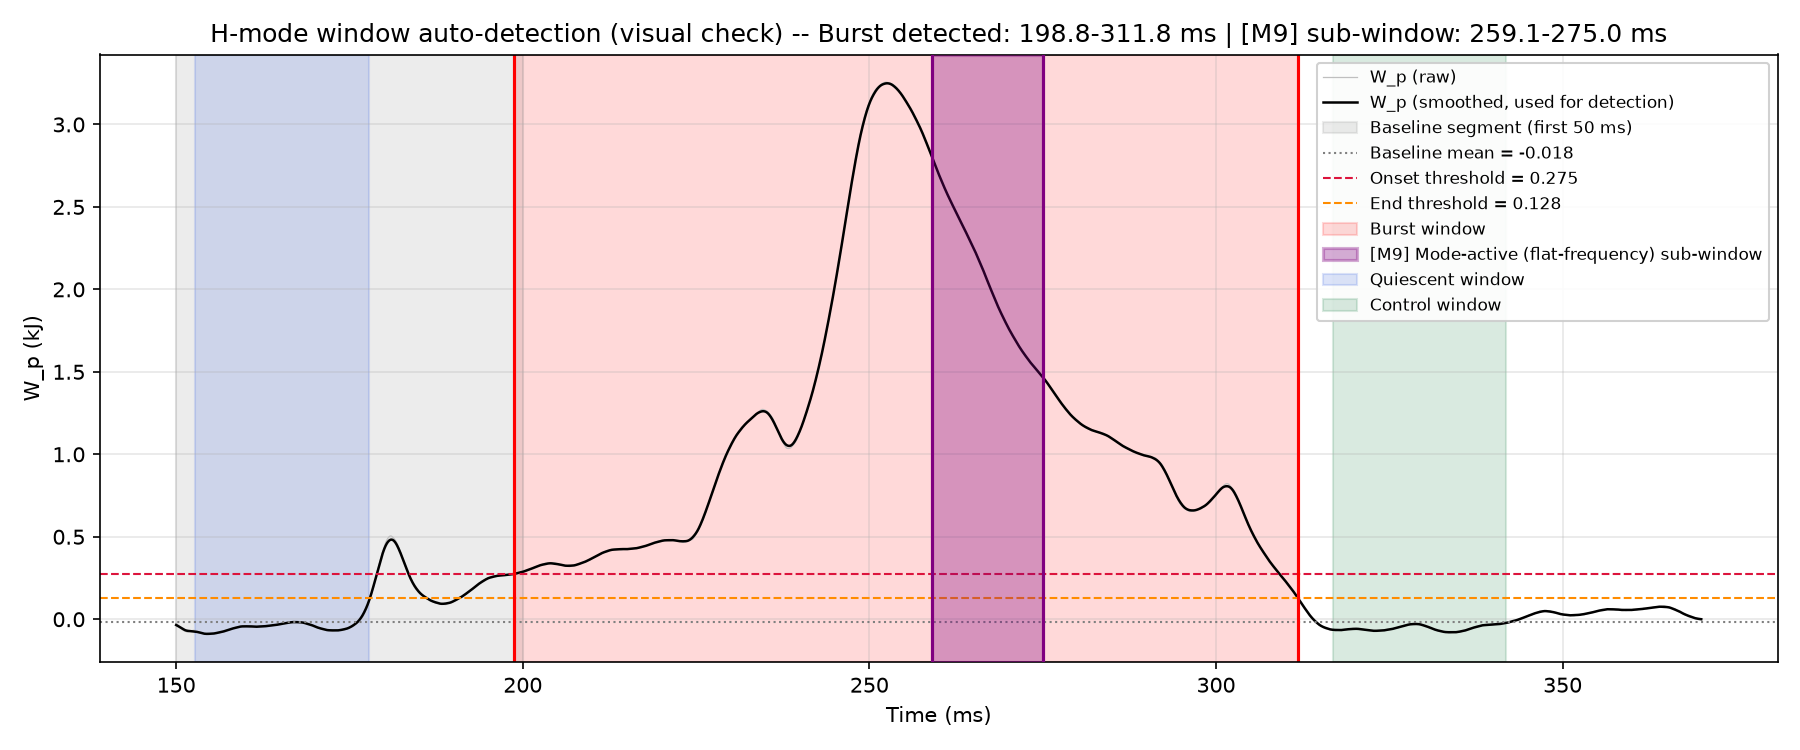
\includegraphics[width=\textwidth,height=0.8\textheight,keepaspectratio]{Images/obj3_nonlinear_coupling/mhd_burst_window_detection_88653.png}
    \end{figure}
\end{frame}

\begin{frame}{Backup: Objective 3 -- Control Windows}
    \centering
    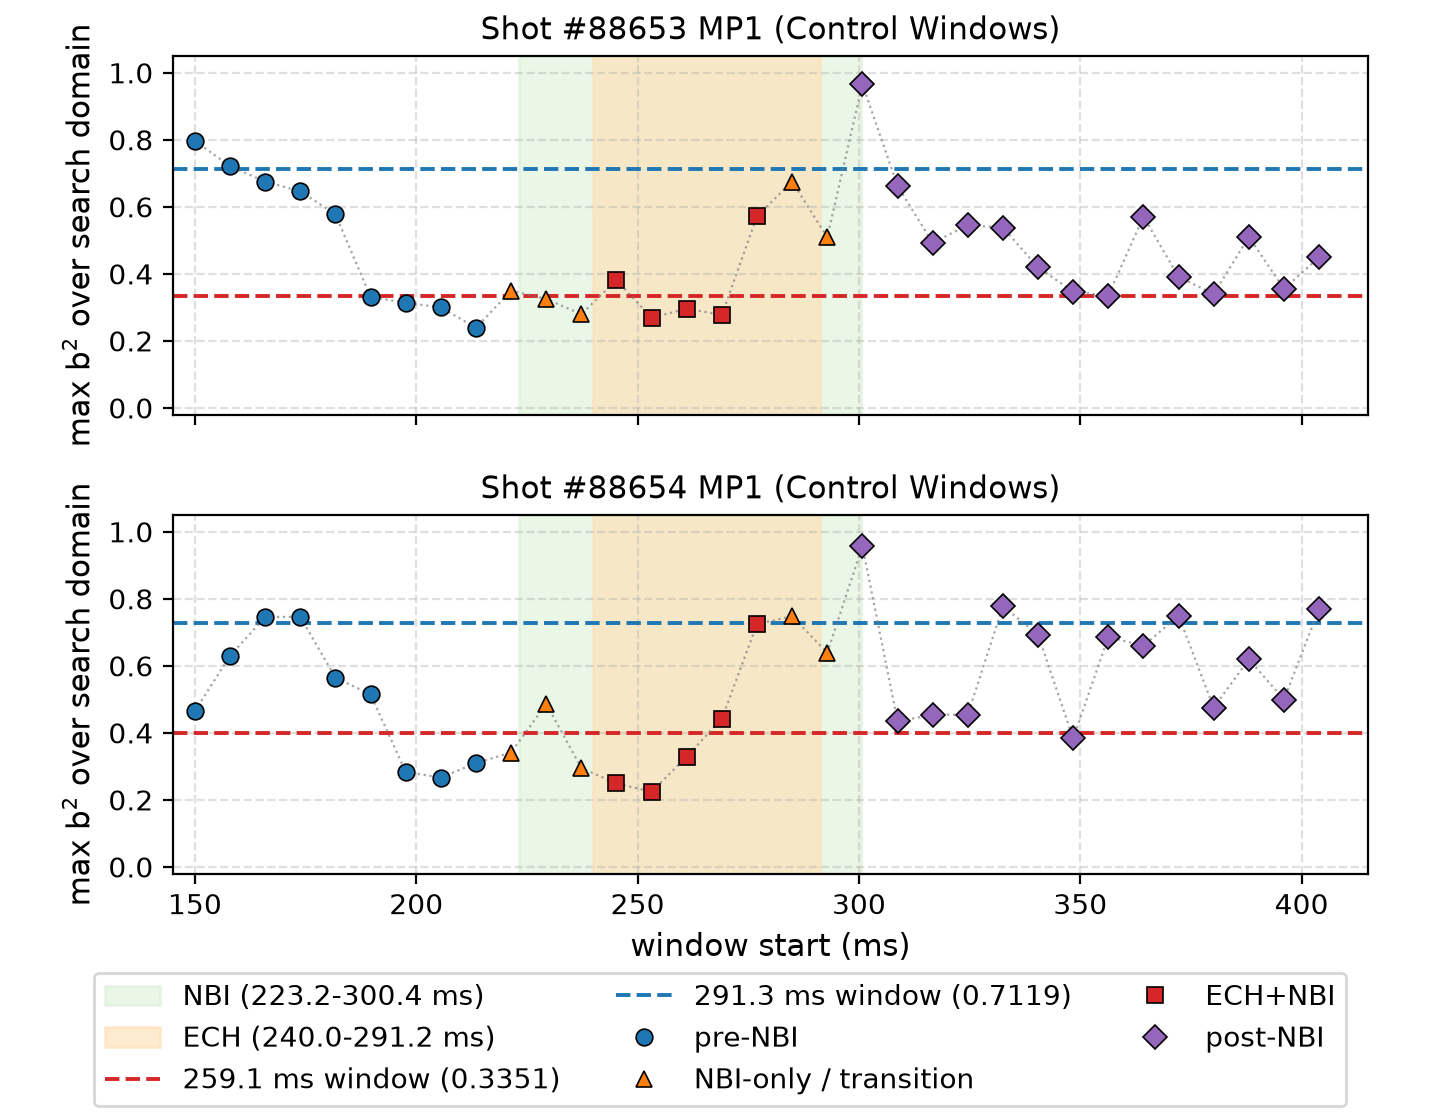
\includegraphics[height=0.70\textheight,keepaspectratio]{Images/obj3_nonlinear_coupling/bicoherence_control_windows_88653_88654.png}
    \vspace{0.05cm}

    {\footnotesize Heated-window maxima (dashed lines) lie within the spread of 33 control windows per shot (median $0.42$ and $0.50$); windows without heating reach $0.80$ and $0.75$.}
\end{frame}

\begin{frame}{Backup: Objective 3 -- Statistical Nuance \& Energy Context}
    \textbf{Burst vs.\ Quiescent \& Control Comparisons}
    \begin{itemize}
        \item \textbf{Energy Transport:} the burst window shows elevated stored
        energy ($\langle W_p\rangle=\SI{2.07}{kJ}$) with a heavily degraded
        derivative ($\langle dW_p/dt\rangle=\SI{-83.24}{kJ/s}$).
        \item \textbf{Bicoherence:} after the estimator correction, no triad in the burst window is distinguishable from the amplitude-conditioned null; the earlier burst-versus-quiescent comparison used the uncorrected routine and is withdrawn.
        \item \textbf{Conclusion:} no link between bicoherence and the stored-energy derivative is claimed.
    \end{itemize}
\end{frame}

\begin{frame}{Backup: Objective 3 -- Shot \#88654 Reproducibility Check}
    \footnotesize
    \textbf{Primary modes reproduce in 88654; the NBI-only maximum does not.}
    Same 259.1--275.0\,ms window, same dual-criterion pipeline, heating
    phase confirmed time-aligned (ECH off 291.2\,ms, NBI off
    300.4--300.6\,ms, identical in both shots).
    \vspace{0.15cm}
    \begin{center}
    \begin{tabular}{cccc}
        \toprule
        88653 $f$ (kHz) & 88654 $f$ (kHz) & Shift & $\gamma^2$ (88653 vs.\ 88654) \\
        \midrule
        40.0 & 37.5 & $-2.5$ & 0.97 vs.\ 0.96 \\
        89.0 & 87.0 & $-2.0$ & 0.85--0.94 vs.\ 0.90--0.96 \\
        45.5 & 43.0 & $-2.5$ & 0.92--0.95 vs.\ 0.85--0.92 \\
        83.5 & 82.5 & $-1.0$ & 0.61--0.82 vs.\ 0.69--0.86 \\
        79.0 & 77.0 & $-2.0$ & 0.43--0.76 vs.\ 0.66--0.89 \\
        \bottomrule
    \end{tabular}
    \end{center}
    \vspace{0.2cm}
    \begin{itemize}
        \item All five dual-criterion modes reproduce 1-to-1 (same rank
        order), downshifted 1--\SI{2.5}{kHz} (consistent with $I_p$
        $\sim$5\% lower in 88654) with comparable or higher inter-probe
        coherence.
        \item Bicoherence in 88654 (corrected estimator, same windows): max $b^2=0.398$ ($p\approx0.14$) and $0.729$ ($p\approx0.08$). The 88653 NBI-only maximum is not reproduced ($b^2=0.083$); the ECH+NBI triad is ($b^2=0.378$, per-bin $p=0.026$), coinciding with a \SI{148}{kHz} burst in both shots. Earlier 88654 values ($b^2\le0.34$) came from the uncorrected routine and are withdrawn.
    \end{itemize}
\end{frame}


\subsection{Backup: Former Conclusions}

\begin{frame}{Backup: Detailed Conclusions}
    \footnotesize
    \begin{itemize}
        \item \textbf{Objective 1:} A single $m=+3$ energetic-particle-like mode at
        $\sim$\SI{89}{kHz} ($n\equiv-1$ (mod 4)) is identified in the
        magnetic data and \textbf{keeps its identity}
        across ECH shut-off -- only its frequency shifts. ECE fluctuation in the mode band
        peaks near $\rho\approx0.62$ but is not coherent with MP1, so radial localization
        is suggestive only.
        \item \textbf{Objective 2:} The mode envelope correlates strongly with heating and
        confinement metrics ($r=0.57$--$0.87$ for $I_p$, $W_p$, $n_e$, H$\alpha$ in both
        bands; consistent with \textbf{NBI drive} rather than ECH), establishing the
        EPM--heating link. The Primary poloidal structure is \textbf{confirmed} ($m=+3$; Secondary
        tentative); band-separated scaling-model tests are inconclusive -- no model is
        statistically significant.
        \item \textbf{Objective 3:} No evidence for three-wave coupling after correcting the estimator: heated-window bicoherence maxima lie within the spread of 33 control windows per shot and of an amplitude-conditioned surrogate null (family-wise $p\ge0.06$); the highest $b^2$ values come from a few segments (ECH-off, NBI-off, a \SI{148}{kHz} burst), and the self-product of the primary has no stable biphase.
        \item \textbf{Confinement relevance:} the primary mode's edge/core
        localization and weak edge-H$\alpha$ coupling ($\gamma^2=0.23$) make it a
        possible fast-ion/heat-loss channel, though a direct transport
        coefficient has not yet been quantified -- a natural next step.
    \end{itemize}
    \vspace{0.2cm}
    \textbf{Next steps:} validate the corrected bicoherence on further shots, test the transfer direction with two-point bispectra, resolve the mode identity, and extend the pipeline to a broader shot database.
\end{frame}

\begin{frame}{Backup: Thesis Objectives -- Status Summary}
    \footnotesize
    \begin{center}
    \renewcommand{\arraystretch}{1.3}
    \begin{tabular}{p{6.2cm}p{5.5cm}c}
        \toprule
        Specific objective (thesis \S1.3.2) & Delivered evidence & Status \\
        \midrule
        Spectral properties \& temporal evolution; dominant modes &
        $m={+}3$ mode at $\sim$\SI{89}{kHz}, $n\equiv{-}1$; survives ECH shut-off &
        \textbf{Met} \\
        EPM--heating correlation; statistical metrics &
        $r=0.57$--$0.87$ vs.\ $I_p$, $W_p$, $n_e$, H$\alpha$; NBI drive $>$ ECH &
        \textbf{Met} \\
        Secondary-band H-mode fluctuations; edge turbulence \& heat-transport coupling &
        Bicoherence: no coupling detected (negative result); edge/H$\alpha$ coupling weak
        ($\gamma^2=0.23$); not reproduced in shot \#88654 &
        \textbf{Negative result} \\
        \bottomrule
    \end{tabular}
    \end{center}
    \vspace{0.3cm}
    \normalsize
    The third objective is a negative result: after correcting the estimator, no three-wave coupling is detected, and no link to edge turbulence or heat transport is claimed.
\end{frame}

\end{document}
